% THE AMAZING BAXTER FEEDING ROBOT 
\documentclass[11pt]{report} %Letter size, letter type and report article structure

\usepackage{geometry}
\geometry{
 a4paper,
 total={210mm,297mm},
 left=40mm,
 right=20mm,
 top=40mm,
 bottom=30mm,
 }
 
\usepackage[spanish, english]{babel} % Recognize Spanish language

\usepackage[utf8]{inputenc} % Recognize Latin characters

\usepackage{amsmath} % Insert math formulas/functions

\usepackage{amsfonts} % Extended set of fonts

\usepackage{graphicx} % Include graphics in document

\usepackage{siunitx} % Consistent set of units with rules on how they are to be used

\usepackage{caption} % Caption for images, formulas and tables
\DeclareCaptionType{equ}[][] % Add caption functionalities to equations

\usepackage{natbib} % Cite library (to reference in APA format)
\usepackage[breaklinks=true]{hyperref} % Handle cross-referencing commands
\urlstyle{same}
\usepackage{url}

\usepackage{dirtytalk} % Add "in quotes" for specific parts of text (add "something")

\usepackage{comment} % Extra big-comments functionalities

\usepackage{textcomp} % For "R" and "TM" symbols

\usepackage{subcaption} % For sub-figures

\usepackage{array} % Usage of arrays
\newcolumntype{M}[1]{>{\centering\arraybackslash}m{#1}} % Center tables vertically

\usepackage{booktabs} % Better quality tables

\usepackage{longtable} % Allow tables to flow over page boundaries

\usepackage{makecell} % Extra functionalities to table cells tabs

\usepackage{multirow} % Extra functionalities to table cells row/cols

\usepackage{float} % Improve figures/tables position in page

\usepackage{algorithm} % Write algorithms easily

\usepackage{blindtext} % Producing 'blind' text for testing

\usepackage[noend]{algpseudocode} % Improve pseudo-code algorithms

\usepackage[dvipsnames,table,xcdraw]{xcolor} % Color things

% Commands to generate list of equations
\usepackage{tocloft} % Package to generate list of equations
\newcommand{\listequationsname}{}
\newlistof{myequations}{equ}{\listequationsname}
\newcommand{\myequations}[1]{%
\addcontentsline{equ}{myequations}{\protect\numberline{\theequation}#1}\par}
\setlength{\cftmyequationsnumwidth}{2.5em}% Width of equation number in List of Equations


% These commands help us generate the "subsubsubseciton{}" title
\newcommand{\subsubsubsection}[1]{\paragraph{#1}\mbox{}\\}
\setcounter{secnumdepth}{4}
\setcounter{tocdepth}{4}


% Extra functionalities for vertical text
\newcommand*\rot{\rotatebox{90}}
\newcommand*\OK{\ding{51}}

% Reestablish specific low-level configurations
\renewcommand\theadalign{cb}
\renewcommand\theadfont{\bfseries}
\renewcommand\theadgape{\Gape[4pt]}
\renewcommand\cellgape{\Gape[4pt]}

% Remove first-indent in all document
\setlength\parindent{0pt}

% Avoid annoying "under full hbox oversize comment"
\hbadness = 2147483647
\vbadness = 2147483647

% Extra math operators values
\DeclareMathOperator{\T}{T}
\DeclareMathOperator{\g}{g}
\DeclareMathOperator{\f}{f}
\DeclareMathOperator{\F}{F}
\DeclareMathOperator{\h}{p}
\DeclareMathOperator{\p}{p}
\DeclareMathOperator{\U}{U}


% ---------------------------------------------------------

\begin{document}

% ---------------------------------------------------------

\begin{titlepage}

\begin{center}

\begin{Large}

\vspace*{1cm}
\textbf{ASSISTED ROBOTICS FOR FEEDING INDIVIDUALS WITH UPPER LIMB DISABILITIES}\\[6.5cm]

\textbf{Santiago García Arango} \\
\textbf{Elkin Javier Guerra Galeano}

\end{Large}

\vfill


\includegraphics[width=6cm]{assets/imgs/logoeia.png}\\

\begin{large}
\textbf{EIA UNIVERSITY}\\
\textbf{MECHATRONICS ENGINEERING}\\
\textbf{ENVIGADO, COLOMBIA}\\
\textbf{2021}\\
\end{large}
\end{center}
\end{titlepage}

% ---------------------------------------------------------

\begin{titlepage}
\begin{center}

\begin{Large}

\vspace*{1cm}
\textbf{ASSISTED ROBOTICS FOR FEEDING INDIVIDUALS WITH UPPER LIMB DISABILITIES}\\[3.5cm]

\textbf{Santiago García Arango}\\
\textbf{Elkin Javier Guerra Galeano}\\[2cm]

\end{Large}

\begin{large}

\textbf{Bachelor's final project to obtain the degree of:}\\
\textbf{Mechatronics Engineer}\\[2cm]

\textbf{Director of the project:}\\
\textbf{Dolly Tatiana Manrique Espíndola, M.Sc., Ph.D.}\\[1cm]

\end{large}

\vfill


\includegraphics[width=5cm]{assets/imgs/logoeia.png}\\

\begin{large}
\textbf{EIA UNIVERSITY}\\
\textbf{MECHATRONICS ENGINEERING}\\
\textbf{ENVIGADO, COLOMBIA}\\
\textbf{2021}\\
\end{large}

\end{center}
\end{titlepage}

% ---------------------------------------------------------

\begin{titlepage}
\begin{center}

\begin{Large}

\vspace*{1cm}
\textbf{ACKNOWLEDGMENTS}\\[3.5cm]

\textbf{Acknowledgments 1}\\

\end{Large}

\begin{Large}

\vspace*{3cm}

\textbf{Acknowledgments 2}\\

\end{Large}

\vfill

\end{center}
\end{titlepage}

% ---------------------------------------------------------

\pagenumbering{arabic} 

\tableofcontents



% ---------------------------------------------------------

\cleardoublepage
\listoffigures

% ---------------------------------------------------------

\cleardoublepage
\listoftables

% ---------------------------------------------------------

\cleardoublepage
\chapter*{List of Symbols}

\begin{longtable}{p{5mm} c p{120mm} }

\multicolumn{3}{l}{\textbf{Position Variables}}\\
\\
$\zeta$ & --- & Vector of something...\\
\\
\multicolumn{3}{l}{\textbf{Robot's parameters}}\\
\\
$P$ & --- & Centroid of ...\\

\\
\multicolumn{3}{l}{\textbf{Control Theory parameters}}\\
\\
$t$ & --- & Time ...\\

\\
\multicolumn{3}{l}{\textbf{Probability functions}}\\
\\
$\g(.)$ & --- & Probability function for ...\\

\\


\end{longtable}

% ---------------------------------------------------------

\cleardoublepage
\chapter*{List of Equations}

\listofmyequations

% ---------------------------------------------------------

\chapter*{Abstract}


The exponential growth of technology has made it possible to achieve new solutions to improve the human beings' quality of life. One of the areas that has experienced the greatest development in the last 20 years is robotics and its derivatives. Currently, there has been a significant increase in the number of people with motor disabilities in the upper limbs, including more than 10 million people with Parkinson's disease and several individuals who, due to other circumstances, have lost the mobility of their upper limbs. This group of people not only have major difficulties in the daily task of feeding, but can also experience severe problems of malnutrition and loss of self-esteem. This is why, in this project, an exploratory research will be conducted focused on the development of an active robotic solution, using Baxter Robot, which can give support in the feeding process for these individuals and, at the same time, has conditions of improvement compared to the robotic alternatives that exist in the current market.\\

This development will seek a positive impact for all individuals who fit within the exposed problem and a design methodology will be carried out, oriented to the search for a scalable solution, with the ability to recognize the position of the mouth of individuals through Computer Vision algorithms and with the advantage of being Open Source. It is expected that, at the end of this research, relevant advances will be generated in the development of active robotic solutions for the assistance of this population and the scientific knowledge of robotics in Colombia and the world.\\


\textbf{Keywords:} Robotics, Computer Vision, Control Theory, Denavit Hartenberg, Algorithms, Software, Anomalies, Active Feeding, Autonomous System.

% ---------------------------------------------------------

\chapter*{Introduction}

The overall population that have upper limb special needs or suffer from motor disabilities are more likely to have problems of malnutrition, a reduction in the performance in the activities of daily living, and loss of self-esteem  \citep{cite_ICBF_technical_article, cite_upper_limb_disabilities_self_steem}.\\

In this research project, we will dive into the design of a possible solution for these problems, using Baxter Robot as an active feeding solution that enables individuals to accomplish of the most important daily life activities: eating.\\

The project's scope covers some important stages for the complete design: \\

\begin{enumerate}
    \item General understanding of the overall design based on human-being needs.
    \item Specific planning and implementation of each sub-system of the complete design.
    \item Practical experiments to validate the functionalities of the designs.
    \item Final results analysis and next steps for future improvements.
\end{enumerate}

Throughout this article, we will be exposing the theoretical and practical steps that were involved in the design of the Baxter Feeding Robot solution.\\

At the end of the article, we will expose the most important ethical and real life considerations of designing a robotics solution that interacts with human beings.

% ---------------------------------------------------------

\chapter{Initial Steps}

\section{Understanding the problem}

\subsection{Problem's context and analysis}

According to the Technical Guide of the Food and Nutrition Component for the Population with Disabilities of the Colombian Institute of Family Welfare (ICBF), this group of individuals are more likely to have nutritional problems \citep{cite_ICBF_technical_article}. Likewise, individuals with upper limb disabilities, have a significant reduction in activities of daily living (especially feeding) and may become impaired in their psychological state \citep{cite_upper_limb_disabilities_self_steem}.\\

It is estimated that there are more than 10 million people with Parkinson worldwide, of which a significant percentage have critical mobility problems in their upper extremities \citep{cite_parkinson_foundation_total_cases}. The incidence of people with Parkinson's disability increases with the age of the individuals, but there is an approximate 4\% of them who are diagnosed before the age of 50 years. According to studies conducted by the Parkinson Foundation (PF), men are more likely than women to have this disease. Another factor that is of relevance to this problem is that there is currently a higher prevalence of pain and disabilities in upper limbs in young university populations, which implies an increase in the group of people who will have joint disabilities in the future and will be more likely to present malnutrition problems due to the difficulties of performing the task of feeding by their own hands \citep{cite_park_active_robot_assisted_feeding}.\\

This is why it is necessary to look for technological solutions that allow this group of individuals to receive support and assistance in daily tasks, especially feeding. Considering this context, a branch of robotics known as \say{Assisted Robotics} is of interest, where robotic systems seek to support individuals with disabilities to perform daily tasks \citep{cite_assited_robotics_stanford_lecture_jaffe}.\\

Advances in assisted robotics have led to the development of various systems that seek to assist people with disabilities in the task of feeding (scooping). There are commercial robotic platforms, which seek to fulfill the need to feed patients with upper limb motor disabilities, but these have a number of limitations that restrict and limit their ideal performance. The best known commercial robotic systems for these tasks, such as Myspoon, Bestic Arm, Meal Buddy, Mealtime and Obi, are passive in nature. This means that they do not have the ability to adapt to the dynamic conditions of the user's mouth position, nor the ability to detect anomalies in the feeding process \citep{cite_park_active_robot_assisted_feeding}.\\

A restriction of great relevance found in commercial robotic systems is that they are not able to adapt their behavior to temporary changes in the position of the user's mouth, because their system is passive, limiting the ability to know this information that is required for a correct feeding action. Another limitation of these systems is that they fail to identify anomalies or strange behaviors in the feeding process, generating additional risks for the patient in case of any emergency or eventuality. Finally, these systems are implemented with restricted code, limiting their modifications in the source code and restricting the possibility of replicating these algorithms for the entire population that may need them.\\

Taking into account this worldwide problem, with the aim of improving the quality of life for individuals who have motor disability problems in upper limbs, it is important and of great relevance to seek an active robotic solution that can support the feeding process of these individuals, with a number of significant improvements over current commercial robotic systems. This solution should be able to adapt its dynamic movements constantly according to the position of the user's mouth, be aware of the environment, check for possible anomalies that may occur in it, be accessible and affordable for the population affected by their motor disabilities, be scalable to any other similar robotic system that is programmable and, similarly, should promote and seek innovation and the technological development of related robotic systems in Colombia and the world.\\

Based on the previous arguments, this research will aim to solve the question of:
How to implement an active robotic system for feeding (scooping) patients with motor disabilities in upper extremities, using the Baxter cobot of the EIA University?\\

In order to find a solution for the lack of active commercial robotic systems for feeding individuals, that also have the ability to adapt their movements according to the position of the user's mouth and the conditions of the environment, based on Mechatronics Engineering, several technological solutions can be proposed to integrate the main branches of electronics, mechanics, control systems and software development, to find an optimal solution to this identified problem \citep{cite_university_eia_general}.\\

This is why it is being proposed to develop a programmed robotic solution, which has an user interface activated by voice commands or friendly buttons, to generate a reliable and safe solution for the needs of people with motor disabilities in the upper limbs, to perform the daily activity of feeding. This solution, being open source, can be easily extrapolated to any programmable robotic platform, generating an additional step in the development of assisted robotic systems.\\

Considering the concept of assisted robotics and the importance of helping these individuals, the answer to provide a viable, scalable and safe solution to this problem is the usage of collaborative robots under the approach of working with humans  \citep{cite_rethink_robotics_baxter_factory_worker}. This can be achieved through various robotic alternatives, but it was decided to use Baxter robot from the company Rethink Robotics, which was developed under the concept of \say{cobot}, that means, a collaborative robot to work together with humans and is available in the laboratories of the university campus \citep{cite_university_eia_general}.\\

Due to the arguments exposed above, we want to look for a solution with the Baxter cobot, using the internal architecture of the software components integrated with the infrastructure offered by this company. This solution must be able to integrate the development of the software architecture, computational algorithms, kinematic models, video processing with computer vision, user interface,  and the necessary connections of these components for the correct implementation of the robotic solution, which will be focused on improving the quality of life of individuals who will benefit from this technology. Likewise, the system will represent a series of elements scalable to any other robotic platform with similar operating conditions and will seek to generate a positive impact on the development of assisted robotic systems for the community.\\

The development of a solution to this problem has multiple benefits, both for individuals with motor disabilities in the upper limbs, as well as for the scientific and medical community in Colombia. That is why, by developing this project, we want to take an additional step in the research and applications of assisted robotics, in order to seek to improve the quality of life of people with motor disabilities in the upper limbs.\\

This contribution can allow a person with these conditions, to perform the essential activity of feeding, without the need of having an external person performing this task. In the same way, this generates an increase in self-esteem and quality of life for these individuals.
At the same time, a key factor of the project is that it will positively contribute to the pursuit of three of the global objectives of sustainable development, especially: \say{Health and well-being}, \say{Industry, innovation and infrastructure} and \say{Reduction of inequalities} \citep{cite_united_nations_sustainable_development}.\\

In addition to the previous reasons, one of the most important motives for carrying out this project is that there is a large gap between the robotics of the leading countries in technology and Colombian robotics. This is why the project will provide a methodological approach for robotics research and a technological progress that can be replicated in any Colombian institution that has access to robotic platforms, generating a community that aims to improve robotic developments at a national level.\\


% ---------------------------------------------------------

\newpage

\section{Research objectives}

In this chapter, we will dive into the objectives of the research that are expected by the end of the project.\\

It is of high importance to have a general and specific planning of the objectives to be developed in the evolution of the project. The following are the structured objectives for the final scope of the solution proposed in this project to obtain the degree of \say{Mechatronics Engineers}.\\

\subsection{General objective}

Implement an active feeding system (scooping) for patients with motor disabilities in upper extremities, using the Baxter cobot of EIA University.

\subsection{Specific objectives}

\begin{enumerate}

\item Generate the smooth paths and trajectories between the position of the tool and the user's mouth, through a face detection system, which returns the absolute coordinates of the user's mouth based on the OpenCV library.

\item Implement a control strategy for tracking the proposed paths and trajectories, through a kinematic processing, to generate the action commands to move the joints of the Baxter cobot and validate its performance with a control algorithm, using the current position of the user's mouth as direct feedback to the system.

\item Design an algorithm for anomaly or error detection in the feeding process, which provides an action signal to stop the system in case of unexpected events.

\item Integrate the sub-systems of path and trajectory generation, control strategy and anomaly detection, using the Robot Operating System (ROS) libraries and tools.

\item Develop an user interface, which enables to send the commands to start the feeding and, if necessary, to stop the process.

\end{enumerate}

% ---------------------------------------------------------

\newpage

\section{Reference framework}

\subsection{Historical background}

Robotics was initially conceived as one of the branches of science with the greatest impact on industrial automation and processes that allow repetitive tasks to be performed. However, the concept of robotics has been expanding its scope and applications, because there are new sectors and scenarios where robots with new objectives and capabilities are becoming more frequent. Some of these scenarios are focused on improving the quality of life of human beings. Two major current scenarios of robotics are: assisted robotics and collaborative robotics \citep{cite_service_robotics_and_human_labor}.\\

Assisted robotics refers to all types of robots that have the ability to collect information from the environment, process that information, and perform tasks or actions that benefit individuals with any type of disability \citep{cite_assited_robotics_stanford_lecture_jaffe}. Based on this definition, it can be concluded that assisted robotics enables the improvement of the quality of life of people with any disability, including the human beings with motor impairments in the upper limbs.\\

The existing studies and researches related to robotics focused on patient feeding have had great advances in the last 10 years. Furthermore , it can be visualized that most current works are directed to the search and improvement of systems for feeding individuals in an active way, i.e., systems that autonomously feed patients \citep{cite_park_active_robot_assisted_feeding}.\\

In order to effectively structure and summarize some of the researches, degree papers and patents related to the topic of assisted robotics, a literature review of the last few years was carried out to collect the objectives, methodologies, solutions, strategies and conclusions of these projects. Some of the most relevant ones are presented below:\\

In the article \say{Active robot-assisted feeding with a general-purpose mobile manipulator: Design, evaluation, and lessons learned} \citep{cite_park_active_robot_assisted_feeding}, published in the scientific journal \say{Robotics and Autonomous Systems 124}, an overview of robotic systems focused on patient feeding is presented, providing a contrast of commercial platforms and those under research and development. In this study, an algorithm and software architecture based on a PR2 robotic manipulator was implemented to achieve autonomous feeding of patients with upper extremity disabilities. The characteristics, methodologies and solutions found in similar projects were presented, making a contrast between them and exposing new proposals that made use of some of the knowledge found by all previous investigations. Besides, the article reflects an exhaustive work with a good overview of previous knowledge to develop similar robotic solutions in the future, as it not only exposes the development of their research in the particular context, but also proposes the most important elements to take into account in assisted robotics projects.\\

Another study of major relevance to the state of the art of assisted robotics is \say{SAM, an Assistive Robotic Device Dedicated to Helping Persons with Quadriplegia: Usability Study} \citep{cite_SAM_an_assisted_robotic_device_to_help_quadriplegia_persons}. In this research, important concepts about assisted robotics and the current delimitation of various robotic applications in this area of knowledge are exposed. Likewise, the authors expose the importance of defining the factors for the success of robotic tasks, since the evaluation of the viability of implementation, is linked to correctly defining the success of the corresponding subroutines. Likewise, several interfaces that can be implemented for quadriplegic users are shown and their advantages and disadvantages are contrasted.\\

Additionally, by researching related studies, a very important element was identified in the development of a robotic system that interacts with individuals: the detection of anomalies. To give context to this feature, two research articles were analyzed, which were \say{A Multimodal Execution Monitor with Anomaly Classification for Robot-Assisted Feeding} \citep{cite_multimodal_execution_monitor_with_anomaly_classification} and \say{A Multimodal Anomaly Detector for Robot-Assisted Feeding Using an LSTM-based Variational Autoencoder} \citep{cite_multimodal_anomaly_detector_for_robot_assisted_feeding_LSTM}. From these scientific papers, we gained a deeper insight into more than 5 mathematical methodologies for strategically detecting anomalies. Similarly, they expose analytical procedures that are of great importance in the structure of algorithms that focus on searching for anomaly patterns, enabling us to have these as a starting point to develop new strategies for future robotic implementations.\\

Regarding patents, the United States patent called \say{Mobile human-friendly assistive robot} \citep{cite_patent_mobile_human_friendly_assistive_robot} was mainly reviewed. In this publication, it was possible to identify a viable structure for the communications architecture developed in assisted robotics projects, enabling the selection of the principal and secondary components in the infrastructure to be developed for robotic projects.\\


A very interesting article for the understanding of assisted robotics projects is \say{Robots for humanity: Using collaborative robots to help people with disabilities} \citep{cite_robot_for_humanity_empower_people_with_disabilities}. In this document, it is exposed the relevance of simplifying the graphical user interface, through the use of mathematical tools such as elliptic coordinates and an interface compatible with sound commands. Similarly, the authors propose a strategic error detection system by translating the forces implemented by the robotic system in different mathematical approaches.\\


\subsection{Theoretical background}

Primarily, it is important to delimit the suggested solution within a specific context, explaining the use cases for the conditions of the technology applied and the people who will benefit from it. A first group of people who benefit are individuals who suffer from advanced Parkinson's disease and are unable to perform smooth feeding movements due to tremors, shaking or bradykinesia in their hands \citep{cite_parkinsons_disease_symptomps_mayo_clinic}. Likewise, there is a large number of people with motor disabilities in upper limbs that fail to be categorized into a specific group of individuals, but because of their age conditions, diseases, symptoms or accidents, they have significant difficulties in the daily process of feeding and can be highly benefited by the technological advances that this solution provides.\\

There are a number of preliminary concepts of critical importance for the understanding and development of the overall project. The most relevant concepts and simple contextualization of these by branches of study are presented below.\\

\subsubsection{Robotic concepts}

Robotics is a field of engineering that has significantly impacted the technological development of manufacture, industrial, medical, security, and human support industries, among others \citep{cite_robots_in_automotive_manufactoring_top_6_applications}. In order to have a solid foundation of the theoretical and mathematical foundations of robotic systems models, it is necessary to go into detail on some concepts and terminology related to the subject. Some of these concepts and terminologies will be discussed in more detail below.\\

\subsubsubsection{Transformation homogeneous matrices}

A transformation matrix is an important mathematical tool to generate expressions of linear systems that have a combination of translational and rotational motions in space.

Given the reference systems \{A\} and \{B\}, with unit vectors that meet the dextrorotating criteria of a linear system, a rotation matrix can be defined as a matrix representation that compacts the rotations that must be performed in space to bring the reference frame {A} to {B} by the three unit vectors expressing the directions of these spatial changes ${_B^A}\hat{X}$, ${_B^A}\hat{Y}$, ${_B^A}\hat{Z}$ \citep{cite_craig_robotics}.\\

To generate the resulting rotation matrix between systems \{A\} and \{B\}, we proceed to create a matrix with the following structure:

\begin{equ}[H]
\begin{equation} \label{eq:rotation_matrix_general_structure}
    _{B}^{A}\textrm{R} = 
    \begin{bmatrix}
    {_B^A}\hat{X} & {_B^A}\hat{Y} & {_B^A}\hat{Z}
    \end{bmatrix} =
    \begin{bmatrix}
    r_{11} & r_{12} & r_{13}\\ 
    r_{21} & r_{22} & r_{23}\\ 
    r_{31} & r_{32} & r_{33}
    \end{bmatrix}
\end{equation}
\myequations{Rotation matrix general structure}
\caption{Rotation matrix general structure}
\end{equ}

As show in equation \ref{eq:rotation_matrix_general_structure}, the rotation matrix structure is a 3 by 3 matrix with orthogonal conditions with determinant 1. These properties are useful to compute some important matrix multiplications for different types of linear problems.\\

The next relevant conceptual step for the creation of a homogeneous transformation matrix is the translation. To represent a translation from a coordinate system to a point P, at least one vector indicating the relative translations of each of the unit vectors governing the orthogonal basis is required $\hat{X}$, $\hat{Y}$, $\hat{Z}$ :

\begin{equ}[H]
\begin{equation} \label{eq:translation_vector_general_structure}
    _{}^{A}\textrm{P} = \begin{bmatrix}
    P_{x}\\ 
    P_{y}\\ 
    P_{z}
    \end{bmatrix}
\end{equation}
\myequations{Position translation vector structure}
\caption{Position translation vector structure}
\end{equ}

Finally, when a mathematical strategy is required to represent both the translation and rotation of a system in space, this transformation can be expressed as a transformation matrix with the following structure:

\begin{equ}[H]
\begin{equation} \label{eq:tranformation_matrix_general_structure}
    _{B}^{A}\textrm{T} = 
    \begin{bmatrix}
    _{B}^{A}\textrm{R} & _{}^{A}\textrm{P}\\ 
    \O  & 1
    \end{bmatrix} = 
    \begin{bmatrix}
    r_{11} & r_{12} & r_{13} & P_{x}\\ 
    r_{21} & r_{22} & r_{23} & P_{y}\\ 
    r_{31} & r_{32} & r_{33} & P_{z}\\ 
    0 & 0 & 0 & 1
    \end{bmatrix}
\end{equation}
\myequations{Transformation matrix general structure}
\caption{Transformation matrix general structure}
\end{equ}

\subsubsubsection{Forward Pose kinematics}

The Forward Pose Kinematics (FPK) transform are all those equations that relate the behavior of a robotic system, taking into account as input parameters the values of each of the joints associated with the degrees of freedom, allowing to obtain as output the absolute Cartesian coordinates for the robot's end effector \citep{cite_craig_robotics}.\\

There are two main techniques for obtaining the Forward Pose Kinematics (FPK) of a robotic system, the geometrical method and the analytical method. In the geometrical method, a set of equations obtained from the model of the robot in the Cartesian space is formulated and a series of expressions is sought to represent the absolute spatial coordinates of the global system, that is, the expected position of the end effector. For this method, it is common to refer to the desired point as \say{Ptool} \citep{cite_craig_robotics}.\\

The analytical approach is a systematic methodology where rigorous steps must be followed to obtain the transformation matrices that govern the robotic system. This approach is divided into three main stages, which are: locating the axes of rotation or translation of each degree of freedom (DOF), defining the origin and direction of rotation of the main axes of each degree of freedom and, finally, locating the missing axes to obtain a series of reference systems that fulfill the desired translations and rotations \citep{cite_barrientos_robotics_book}.\\

The following is an example of the FPK of a revolute-revolute planar robot:

\begin{center}
\includegraphics[width= 0.4\textwidth]{\string "assets/pdfs/reference_framework/RR_general_draw".pdf}
\bigbreak
\begin{minipage}{\linewidth} %Keep image/PDF in only 1 page
\captionof{figure}{General schematic model for RR planar robot.}\label{fig_general_rr_drawing.}
\end{minipage} \end{center}

By solving the FPK of the RR robot, from fig[\ref{fig_general_rr_drawing.}], it can be shown that the equations governing the position and orientation of the robot tool are the following:

\begin{equ}[H]
\begin{equation} \label{eq:results_rr_robot_fpk_example}
    \begin{split}
        P_{Tx} & = L_{1} \cdot cos(\theta_{1}) + L_{2} \cdot cos(\theta_{1} + \theta_{2}) \\
        P_{Ty} & = L_{1} \cdot sin(\theta_{1}) + L_{2} \cdot sin(\theta_{1} + \theta_{2}) \\
        \alpha & = \theta_{1} + \theta_{2}
    \end{split}
\end{equation}
\myequations{Forward Pose Kinematics results for RR robot example.}
\caption{Forward Pose Kinematics results for RR robot example.}
\end{equ}

\subsubsubsection{Inverse Pose Kinematics} \label{baxter_inverse_pose_kinematic}

The Inverse Pose Kinematics (IPK), are all those equations that relate the behavior of a robotic system, having as input parameters the absolute Cartesian values, allowing finding the equivalent values of each one of the degrees of freedom (DOF) of a robotic system \citep{cite_craig_robotics}.

It is common for a robot to have different kinds of actuators for the linear and rotational movements of its joints, so it is of high importance to obtain a series of expressions that can describe the possible values of these joints, for a specific position of the robot's tool.\\

Based on the following schematic, we can find the IPK of the given RR robot example:

\begin{center}
\includegraphics[width= 0.4\textwidth]{\string "assets/pdfs/reference_framework/RR_angles_convention".pdf}
\bigbreak
\begin{minipage}{\linewidth} %Keep image/PDF in only 1 page
\captionof{figure}{General schematic with the angles convention for RR planar robot.}\label{fig_rr_angles_exmple_schematic}
\end{minipage} \end{center}


The equations that describe the IPK of a planar RR robot, as shown in Fig[\ref{fig_rr_angles_exmple_schematic}], are shown as follows:

\begin{equ}[H]
\begin{equation} \label{eq:results_rr_robot_ipk_example}
    \begin{split}
        L_{T} & = \sqrt{P_{Tx}^2 + P_{Ty}^2} \\
        \gamma & = atan2(P_{Tx}, P_{Ty}) \\
        \alpha & = acos \left( \frac{L_{T}^2 + L_{1}^2 - L_{2}^2}{2 \cdot L_{1} \cdot L_{T}} \right) \\
        \beta & = acos \left( \frac{L_{1}^2 + L_{2}^2 - L_{T}^2}{2 \cdot L_{1} \cdot L_{2}} \right) \\
        \theta_{1} & =  \gamma + \alpha \\
        \theta_{2} & = \beta - \pi
    \end{split}
\end{equation}
\myequations{Inverse Pose Kinematics results for RR robot example.}
\caption{Inverse Pose Kinematics results for RR robot example.}
\end{equ}

It's important to state that in robotic systems with more than one degree of freedom, it is possible to reach the same point in space through different configurations of its joints, usually known as \say{elbow up} and \say{elbow down} for the same joint. For this reason, it should be kept in mind that there could be more possible solutions, as more degrees of freedom are available.\\

\subsubsubsection{Path planning}

Path planning refers to the strategy of generating spatial routes to achieve the movements of a robotic system between two points in space, using techniques to find the most appropriate route, taking into account the constraints of the environment. The methods to generate the paths may vary according to the type of robot and the dynamic conditions that it has to face in the context of the surrounding environment. It is relevant to mention that, in order to generate the planning of a given path, a series of preliminary elements of the environment must be previously known through integrated sensors that are able to translate their signals into valuable information for the robot \citep{cite_wheeled_robots_autonomous_book}.\\

\subsubsubsection{Higher-order polynomials trajectories}

Soft trajectories are parametric vectors that define all the points in space that a robotic manipulator must follow, in order to change its position in space from an initial point to an final point, having as input the desired position, velocity and acceleration conditions. There are two mathematical trajectories that allow an acceptable robotic performance, these are the 3\textsuperscript{rd} and 5\textsuperscript{th} order trajectories. The 5\textsuperscript{th} order trajectories are those that allow the control of any kind of dynamic system, with a correct control of variables such as jerk \citep{cite_craig_robotics}.
In this section, it is important to understand in depth the mathematical expressions that govern a behavior with 3\textsuperscript{rd} and 5\textsuperscript{th} order trajectories.\\

The 3\textsuperscript{rd} order trajectories fulfill the following mathematical expressions:


\begin{equ}[H]
\begin{equation} \label{eq:equations_for_third_order_trajectories}
    \begin{split}
        \theta(t) &= a_{0} + a_{1} \cdot t + a_{2} \cdot t^2 + a_{3} \cdot t^3\\
        a_{0} &= \theta_{0}\\
        a_{1} &= \dot{\theta_{0}} \\
        a_{2} &= \frac{3(\theta_{f} - \theta_{0})}{t_{f}^2} - \frac{2 \dot{\theta_{0}}}{t_{f}} - \frac{\dot{\theta_{f}}}{t_{f}}\\
        a_{3} &= \frac{2(\theta_{0} - \theta_{f})}{t_{f}^3} + \frac{(\dot{\theta_{0}} + \dot{\theta_{f}})}{t_{f}^2}
    \end{split}
\end{equation}
\myequations{Equations for third order trajectories.}
\caption{Equations for third order trajectories.}
\end{equ}

Similarly, the 5\textsuperscript{th} order polynomial trajectories, follow these mathematical equations:


\begin{equ}[H]
\begin{equation} \label{eq:equations_for_fifth_order_trajectories}
    \begin{split}
        \theta(t) &= a_{0} + a_{1} \cdot t + a_{2} \cdot t^2 + a_{3} \cdot t^3 + a_{4} \cdot t^4 + a_{5} \cdot t^5\\
        a_{0} &= \theta_{0}\\
        a_{1} &= \dot{\theta_{0}} \\
        a_{2} &= \frac{\Ddot{\theta_{0}}}{2}\\
        a_{3} &= \frac{20\theta_{f} - 20\theta_{0} - (8\dot{\theta_{f}} + 12\dot{\theta_{0}})t_{f} - (3\ddot{\theta_{0}} - \ddot{\theta_{f}})t_{f}^2}{2t_{f}^3}\\
        a_{4} &= \frac{30\theta_{0} - 30\theta_{f} + (14\dot{\theta_{f}} + 16\dot{\theta_{0}})t_{f} + (3\ddot{\theta_{0}} - 2\ddot{\theta_{f}})t_{f}^2}{2t_{f}^4}\\
        a_{5} &= \frac{12\theta_{f} - 12\theta_{0} - (6\dot{\theta_{f}} + 6\dot{\theta_{0}})t_{f} - (\ddot{\theta_{0}} - \ddot{\theta_{f}})t_{f}^2}{2t_{f}^5}
    \end{split}
\end{equation}
\myequations{Equations for fifth order trajectories.}
\caption{Equations for fifth order trajectories.}
\end{equ}



\subsubsubsection{Assistive robotics}

A collaborative robot or \say{cobot} is a robotic device capable of manipulating objects in cooperation with or providing assistance to humans. Thus, cobots have the ability to perform critical tasks for humans or work in conjunction with them \citep{cite_robots_for_collaboration_with_human_operators}. A field of collaborative robotics is assisted robotics, defined as any robotic device that performs tasks for the benefit of people with disabilities in the context of activities of daily living \citep{cite_assited_robotics_stanford_lecture_jaffe}.\\

\subsubsubsection{Robot's workspace}

In the context of robotics, the workspace is defined as all possible spatial locations where a robotic manipulator is able to reach thanks to the strategic movement of its degrees of freedom independently. The mathematical delimitation of this is a process that requires finding multiple possible spatial solutions for the maximum access points and plotting them in a simulation environment. It is common for manufacturers of industrial robots to provide a detailed review and explanation of the workspace in the robot's data-sheets, because it varies not only by geometric constraints, but also by the mechanical restrictions existing in the joint connections \citep{cite_craig_robotics}.\\


\subsubsubsection{Baxter cobot}

Baxter is a collaborative robot developed for the industrial sector by the company Rethink Robotics. It was designed with a series of sensors, cameras and control systems that allows it to work in a cooperative environment and to adapt easily to its workspace \citep{cite_rethink_robotics_official_page}.\\

Baxter was announced to the community in September 2011 and can be broadly defined as a two-armed robot with 7 degrees of freedom in each arm. Baxter was introduced to the market as a robot specialized in simple collaborative tasks, such as loading and unloading, organizing and interacting with materials \citep{cite_sdk_baxter_rethink_robotics}. Likewise, being a robot that seeks to interact with humans, it has a screen that simulates the face of the Baxter cobot and additional safety protection features that will be considered in the development of the project.

\begin{figure}[H]
    \centering
    \includegraphics[width=0.65\linewidth]{assets/imgs/reference_framework/baxter_front_view_general_photo.png}
    \caption{Front view for Baxter cobot. Taken at EIA University Laboratory.} 
    \label{fig_baxter_main_image}
\end{figure}

Considering the general specifications, it is of major relevance to have a clear understanding of each one of the degrees of freedom that the Baxter joints have and their standard nomenclatures for their operation. The following figure is an image of the official technical data-sheet of Baxter's documentation, where the seven DOF and their names are illustrated:

\begin{figure}[H]
    \centering
    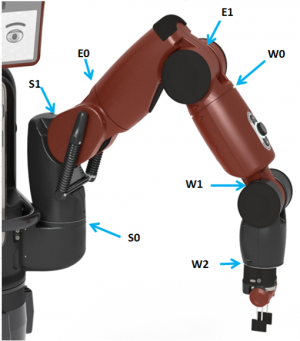
\includegraphics[width=0.4\linewidth]{assets/imgs/reference_framework/baxter_joint_names.png}
    \caption{Baxter left joint names for each DOF. Taken from \citep{cite_baxter_joint_names_from_sdk_wiki}.} 
    \label{fig_baxter_joint_names}
\end{figure}

When working and programming the Baxter cobot, it is essential to have a good understanding of the workspace conditions and the general restrictions of each of the degrees of freedom. The following image is a visual illustration of Baxter's workspace and its numerical limits for each joint:

\begin{figure}[H]
    \centering
    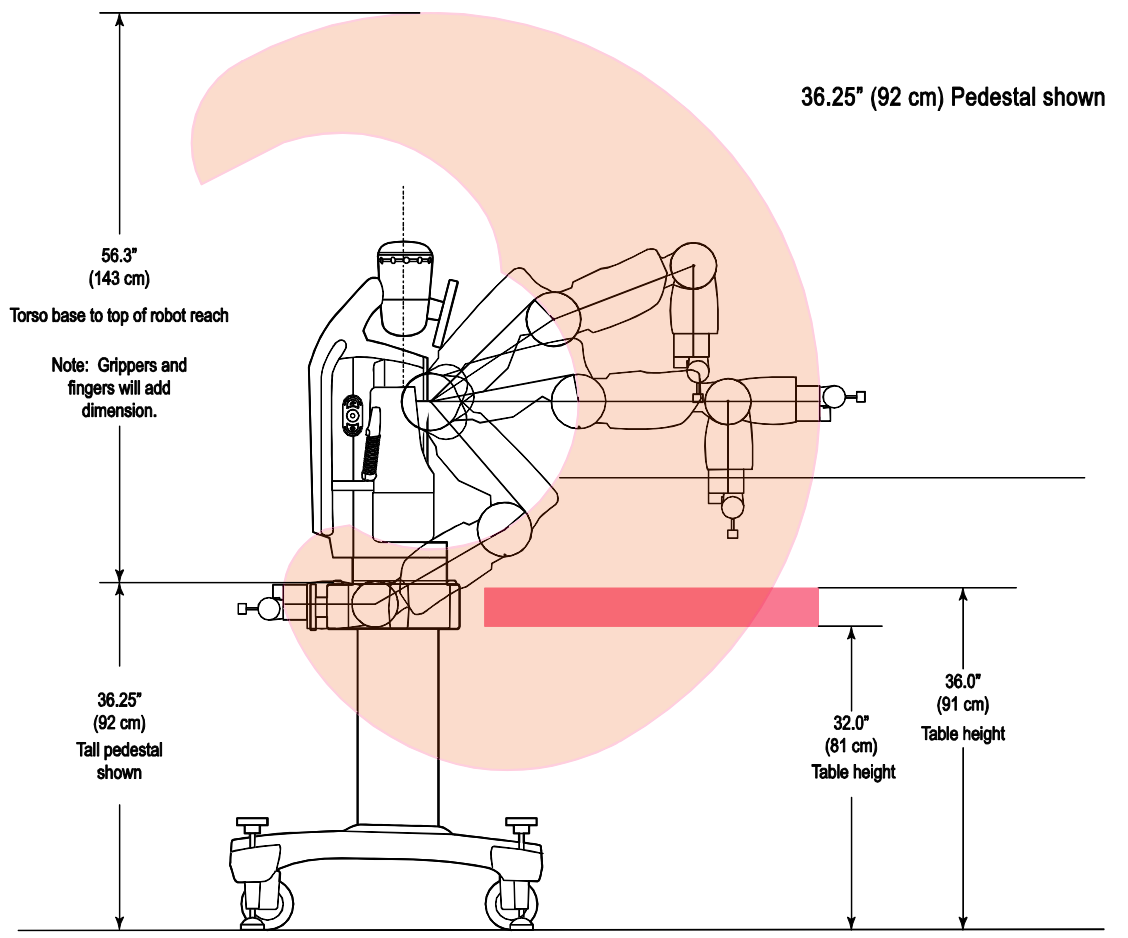
\includegraphics[width=0.65\linewidth]{assets/imgs/reference_framework/baxter_workspace_side_view.png}
    \caption{Baxter workspace side view. Taken from \citep{cite_baxter_workspace_from_sdk_wiki}.} 
    \label{fig_baxter_workspace_1}
\end{figure}

\begin{figure}[H]
    \centering
    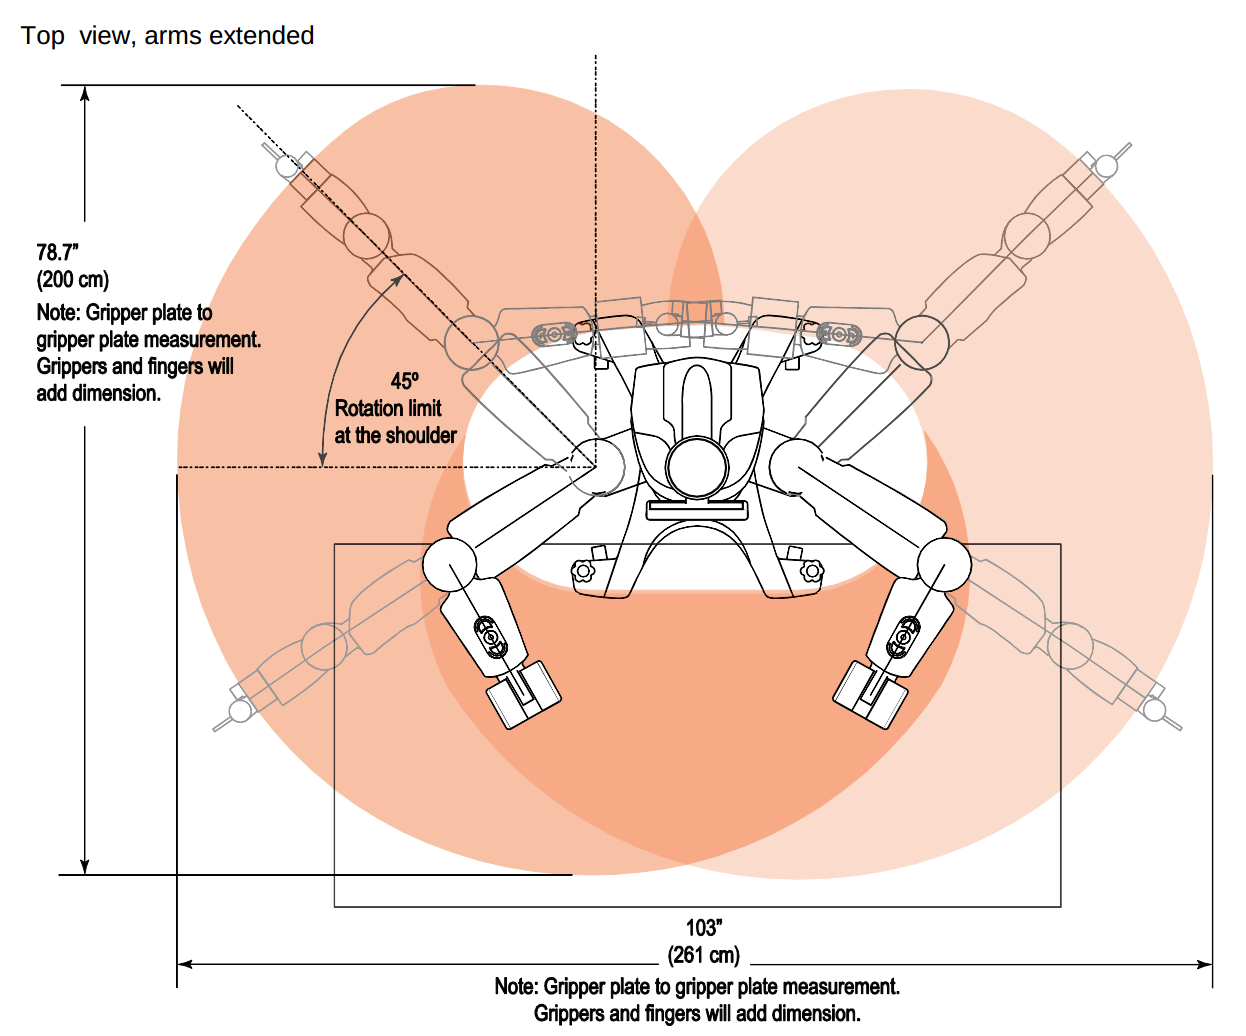
\includegraphics[width=0.65\linewidth]{assets/imgs/reference_framework/baxter_workspace_top_view.png}
    \caption{Baxter workspace top view. Taken from \citep{cite_baxter_workspace_from_sdk_wiki}.} 
    \label{fig_baxter_workspace_2}
\end{figure}


\subsubsection{Software concepts}

In most robotic systems, it is critical to implement a series of algorithms, data-structures and architectures that allow the consistent and safe development of the robot's actual performance. These commands must be programmed through various software schemes and strategies, which are integrated with the electronic and mechanical components that govern the robot's joints and sensors. For this reason, the development of this project should be explained in a comprehensive way, from a software approach.\\

\subsubsubsection{Python}

Python is a multi-platform programming language, developed by Guido van Rossum in 1989 and formalized to public in 1991. It is interpreted, with the ability to update itself dynamically. Its philosophy is based on the simplicity and readability of the codes, allowing several programming paradigms, such as: object-oriented programming, imperative programming and functional programming. It has the advantage of being open source with a significant worldwide community \citep{cite_python_official_site}.\\

\begin{figure}[H]
    \centering
    
\includegraphics[width=0.3\linewidth]{assets/imgs/reference_framework/python_logo_main.png}
    \caption{Python official logo. Taken from \citep{cite_python_official_site}.} 
    \label{fig_python_main_logo}
\end{figure}

The advantage of using a language that is open source and with a flourishing community, is that there are a large number of libraries and tools that are fully accessible, in order to simplify and increase the development of technological solutions based on them. This is why, with the implementation of a single main syntax, multiple solutions can be achieved for software development approaches, such as graphical interfaces, web backend servers, the usage of simulation environments, artificial intelligence and computer vision algorithms.\\

\subsubsubsection{Robot Operating System (ROS)}

ROS stands for \say{Robot Operating System}, which is a set of tools, libraries and open source software for the management of robotic systems. These tools seek to standardize, simplify and perform robust robotic tasks through simple operating protocols for nodes and topics integration. ROS was built with the objective of improving and facilitating the development of software for collaborative robots and there is a growing open source community, which allows the migration of a large number of legacy technologies to these new tools \citep{cite_ROS_official_site}.\\

\begin{figure}[H]
    \centering
    
\includegraphics[width=0.4\linewidth]{assets/imgs/reference_framework/ros_main_logo.png}
    \caption{ROS official logo. Taken from \citep{cite_ROS_official_site}.} 
    \label{fig_ros_main_logo}
\end{figure}

In the context of a Robot Operating System, a node refers to an executable program used to communicate with other nodes through a \say{client} type resource library. There are also \say{messages}, which allow subscribing or publishing native information in ROS to a \say{topic}. Finally, topics are buses of information on which nodes exchange messages \citep{cite_ROS_understanding_nodes}.\\

In any program that has a ROS infrastructure and architecture, there is a main element known as the \say{master}, which aims to verify and validate that the operation of the nodes and their networks for communication are performing their corresponding tasks and properly integrating with each other \citep{cite_ROS_understanding_nodes}.\\


\subsubsection{Computer Vision Concepts}

Computer Vision represents one of the most important fields in the robotic development of projects that must be able to detect dynamic conditions in a given environment. For the correct implementation and execution of this research, the fundamental and relevant concepts within this area of knowledge must be taken into account.\\

\subsubsubsection{Overview of Computer Vision}

Computer vision can be defined as the branch of study responsible for extracting information from one or multiple images through computational algorithms. There are many areas where it is applied, one of the most complicated being the creation of robotic trajectories, where this information is used to control robotic manipulators or autonomous vehicles \citep{cite_computer_vision_advances_in_computers}.\\

One of the most important applications of computer vision is face detection and face recognition. This utility allows detecting a human face through relevant features found by image processing. It can be divided into two processes: identification of an unknown face and validation of a specific face that can be found encoded in a database \citep{cite_computer_vision_techniques_for_face_recognition}. In this project, it will be implemented a face-detection algorithm.\\

\subsubsubsection{Face detection algorithms}

Face detection is a specific field of computer vision algorithms that involve Machine Learning. The main purpose of this field is to estimate the face position and direction from a given image \citep{cite_face_detection_science_direct_article}. Facial recognition algorithms started around 1960s and there have been multiple improvements of different approaches to solve the objective of detecting human faces.\\

One of the most recognized and significant article in the history of face detection is the famous \say{Rapid object detection using a boosted cascade of simple features}, popularly known as \say{Viola–Jones object detection framework} \citep{cite_viola_jones_face_detection_algorithm}. This algorithm enabled the fast processing of digital images with great accuracy via machine learning algorithms for object detection.\\

Viola Jones Algorithms, established three main relevant literature contributions \citep{cite_viola_jones_face_detection_algorithm}. These are:\\

\begin{enumerate}
    \item The introduction of a new image abstraction known as the \say{Integral Image}. This allowed the quick processing of an analyzed image.
    \item A learning algorithm that is based on \say{AdaBoost}, that selects few relevant features from a big data-set and enables an efficient classifier.
    \item A innovative method to combine separate classifiers that increased their complexity in a cascade approach. These allowed the background sections of an image to be discarded quickly in the process of detection.\\
\end{enumerate}

Taking into account these considerations, most modern algorithms use features that were developed by Paul Viola and Michael Jones and evolved their specific classifiers in diverse aspects. One example of the importance of these features is the recognized open-source project called \say{OpenCV}, that implements some variants of these algorithms in their previously trained \say{Face Detection} libraries \citep{cite_opencv_classifier_face_detection_general}.\\



\begin{figure}[H]
    \centering
    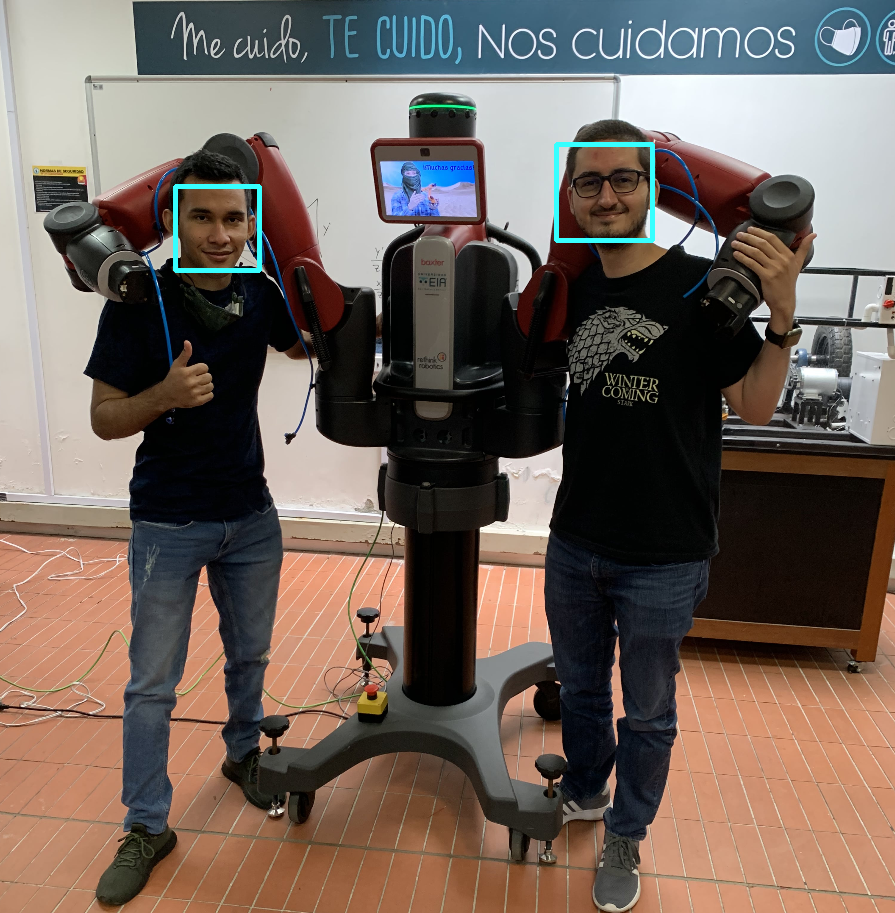
\includegraphics[width=0.8\linewidth]{assets/imgs/reference_framework/face_detection_example_us.png}
    \caption{Face detection algorithm in action. Own development.}
    \label{fig_face_detection_us_with_baxter}
\end{figure}


\subsubsubsection{Stereoscopic Camera}

These are frames acquisition devices, which have the ability to acquire images or videos, while being able to identify the spatial quality associated with a third dimension, i.e., they are able to capture the depth of the surfaces of the image. These cameras use strategies based on the morphology of mammalian eyes to map a three-dimensional structure of the captured scene \citep{cite_stereoscopic_camera_techniques}.\\

\begin{figure}[H]
    \centering
    \includegraphics[width=0.4\linewidth]{assets/imgs/reference_framework/vuze_stereo_camera.jpeg}
    \caption{Vuze stereo camera 3D device. Taken from \citep{cite_photo_vuze_stereo_camera_device}.} 
    \label{fig_vuz_stereo_camera_device}
\end{figure}


\subsubsection{Control theory concepts}

Within the framework of preliminary knowledge for the development of this research, it is very important to have a solid prior knowledge of classical control theory, in order to propose and validate robust control strategies that attempt to achieve the correct trajectory tracking of the dynamic system to be implemented.\\

\subsubsubsection{Motion control systems}

A motion control system aims to follow a given defined trajectory and seeks to reduce the error between the actual performance of the system and its planned trajectory. This control system is very important at the industrial level and are usually guided by 3 integrated control loops: position, velocity and torque. These motion control tasks have a high degree of complexity and usually involve variables such as system load, actuator saturation and robot workspace limitations \citep{cite_position_control_for_linear_motion_servo_systems}.\\

\subsubsubsection{Decentralized control systems}

A decentralized control system is one that has the ability to integrate multiple independent control systems and handle these global inputs to a master processing of each of the individual controllers, allowing the generation of independent control events managed by a master algorithm \citep{cite_centralized_control_systems_book}.\\

\subsubsubsection{Impedance control systems}

In the context of a motion control system, there is a relevant term known as \say{impedance}. This concept refers to the relationship between force and position and/or velocity variables. Taking into account this definition, a completely rigid system is one that has simple impedance.\\

Based on these concepts, an impedance control seeks to carry out an intermediate regulation between the force variables of a system, applied to the desired positions in a specific trajectory. The underlying goal of this control strategy is to assign a prescribed dynamic behaviour of the motion system while its components are interacting with their environment \citep{cite_canudas_theory_of_robotic_control}.\\

Impedance control seeks to model a real-life system into a \say{Generalize Dynamic Impedance}, by a set of linear or non-linear second order differential equations representing a spring-damper-mass system \citep{cite_canudas_theory_of_robotic_control}.\\

\begin{figure}[H]
    \centering
    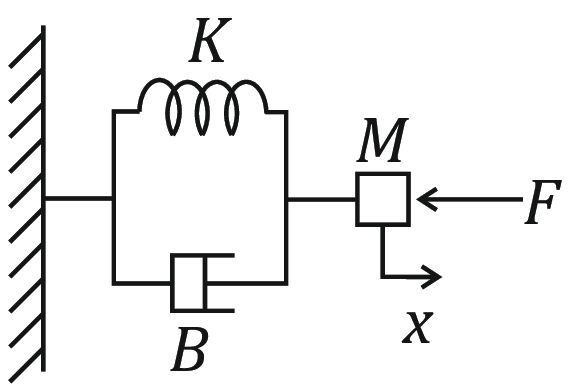
\includegraphics[width=0.4\linewidth]{assets/imgs/reference_framework/mass_damper_mass_system_for_impedance_control.png}
    \caption{Abstraction model of motion system for implementing an Impedance Controller. Taken from \citep{cite_mass_spring_damper_system_ic}.} 
    \label{fig_mass_spring_damper_system}
\end{figure}


\subsubsubsection{Model predictive controller}

Model Predictive Controllers, known as MPC, are control algorithms in which the dynamics of the system must be known through a previous identification of itself, by traditional methods of system identification. These algorithms have advantages such as simplicity, robustness, convenience in implementation, taking into account the system's constraints and a good handling of Multiple-Inputs/Multiple-Outputs (MIMO) systems.\\

Model Predictive Controllers seek to predict the changes in the dependent variables of the system model, which will be caused by the influence of the changes in the independent variables of the system. Similarly, they are widely used in systems with multiple constraints, such as those in which the actuators or sensors have saturation points \citep{cite_mpc_industrial_processes_automation_systems}.\\

MPC literature has been developed significantly over the last decades. One of the reasons that impulsed the community research in MPC algorithms is attributed to the fact that MPCs is a wide-open domain. It integrates and involves: optimal control, control processes, stochastic control, multi-variable control and future set-points of variables \citep{cite_model_predictive_control_camacho_bordons}.\\ 

One great advantage of Model Predictive Controllers is the fact that they allow to predict a behaviour based on a prediction horizon that considers input constraints of the system and the affected variables. This is done with linear and non-linear processes, allowing MPC to interact with a lot of important industrial processes.\\

Another great conditions that has been a golden-key for the development of MPC algorithms, are the fact that embedded system's processors are being improved with exponential characteristics over the last years. This has come with the circumstance that there are plenty of open-source projects that implement the mathematical approach of convex-optimization problems, an intermediate feature in MPC control strategies.\\


\begin{center}
\includegraphics[width= 1.01\textwidth]{\string "assets/pdfs/reference_framework/mpc_general_graph".pdf}
\bigbreak
\begin{minipage}{\linewidth} %Keep image/PDF in only 1 page
\captionof{figure}{General Model Predictive Control plot for relevant variables. Taken from \citep{cite_mpc_article_plot_thermal_control}.}\label{fig_general_mpc_explained_plot_thermal_article}
\end{minipage} \end{center}




% ---------------------------------------------------------

\newpage

\chapter{Methodology}

 There are several methodologies for scientific design to carry out a process of research divulgation. In this investigation it was decided to implement a methodology applied to engineering processes, where there are a series of iterative designs that seek to achieve a final detailed product \citep{cite_dieter_engineering_design}.\\
 
It is also important to point out that the development of this research will have an exploratory approach to the technological and practical solution of the problem to be solved, so the design stages focused on the market study and the financial components to generate a start-up plan at a commercial level will not be developed. Because of this statements, these two stages will be left as a proposal for future research.\\

\section{User requirements identification}

The selection process of the most relevant characteristics in terms of user requirements was carried out taking into account the existing literature on assisted robotics focused on feeding-systems and the general considerations that were determined to be relevant for the considerations of Baxter robot. In this choice for the user requirements, the following needs were identified:\\


\begin{table}[H]
\scalebox{0.78}{
    \begin{tabular}{|c|c|c|c|}
    \hline
    \rowcolor[HTML]{C0C0C0} 
    \textbf{\#} & \textbf{Requirements}                                                    & \textbf{Relevance} & \textbf{Measurement} \\ \hline
    1           & User must feel safe                                                      & 5                  & Subjective           \\ \hline
    2           & System must be able to be initialize through an user-interface           & 4                  & Objective            \\ \hline
    3           & System must be able to detect the user's mouth                           & 5                  & Binary               \\ \hline
    4           & System must be able to generate a trajectory between two points in space & 5                  & Objective            \\ \hline
    5           & System must be able to measure the current end-effector's position       & 5                  & Objective            \\ \hline
    6           & System must be able to move the end-effector following a trajectory      & 5                  & Objective             \\ \hline
    7           & System must be able to move the end-effector close to the user's mouth    & 5                  & Objective            \\ \hline
    8           & System must be able to stop in case of an anomaly detection              & 5                  & Subjective           \\ \hline
    \end{tabular}
}
\caption{\label{tab:user_requirements} User requirements for active feeding system.}
\end{table}


\section{House of Quality}

The House of Quality (HoQ), is a design tool that enables a simple and powerful approach for a \say{quality function deployment}. The tool was originated at the Mitsubishi’s Kobe shipyard site and it has helped the development of multiple industrial solutions, such as home appliances, infrastructures, electronics, clothing, integrated circuits and more \citep{cite_house_of_quality}.\\

The methodology of a House of Quality, maps the corresponding requirements with important engineering conditions that are measurable. The result of these characteristics, generate two important parts: the main matrix and the roof correlation matrix. These matrices are important to understand the underlying relationships and their importance in a measurable way.\\

The result of the HoQ for an active feeding system for patients with motor disabilities in upper extremities, can be seen at fig[\ref{fig_hoq}].\\

\begin{center}
    \includegraphics[width= 0.98\textwidth]{\string "assets/pdfs/methodology/HoQ".pdf}
    \bigbreak
    \begin{minipage}{\linewidth} %Keep image/PDF in only 1 page
    \captionof{figure}{HoQ for an active feeding robotic system. Own development.}\label{fig_hoq}
\end{minipage} \end{center}

As a general conclusion for the House of Quality design analysis, it is important to notice that the three most important engineering conditions are:\\

\begin{enumerate}
    \item Robot's processor (GHz)
    \item Robot's accuracy for joint-encoders (rad)
    \item Robot's memory (RAM)
\end{enumerate}

As a general result, the camera conditions are similarly important and there is no significant difference on the relative relevance for those aspects. As well as that, the robot's payload is not a key aspect, because there is no need for high amounts of robotic load to manipulate.\\


\section{System architecture}

Having an understanding of the overall system's architecture is a key element in the development and analysis of an engineering solution. A block diagram of the complete system will be shown below to understand the signals and information that govern the proposed design.


\begin{center}
\includegraphics[width= 1.01\textwidth]{\string "assets/pdfs/methodology/GeneralBlockDiagram".pdf}
\bigbreak
\begin{minipage}{\linewidth} %Keep image/PDF in only 1 page
\captionof{figure}{General system architecture. Own work.}\label{fig_general_block_diagram}
\end{minipage} \end{center}

As it can be seen in fig[\ref{fig_general_block_diagram}], the main input to the whole system is the action command generated by the user through the user interface. After these action commands are sent, the interface will transform them into signals that initialize the control processes, which enables the robot's strategic motion, depending on the current system conditions.\\

It is important to clarify that the current position of the user's mouth is identified from the robot's sensors, allowing the system to process the video from its cameras, find the position of the mouth and send it to the control algorithm.\\

Similarly, there is an anomaly detector, which is constantly monitoring the current conditions of the system (i.e. control algorithms, Baxter conditions and computer vision algorithms) in order to stop the process in case of any abnormal condition that could harm the patient.\\


\section{Morphological matrix}

The morphological matrix is a powerful tool that makes it possible to generate solutions based on potential variations in a problem's characteristics \citep{cite_morphological_matrix}.\\

For our design, the main problems or conditions are detected from the general block diagram seen in fig[\ref{fig_general_block_diagram}]. These are the main problems to evaluate the best solutions for our specific context. In the following sub-sections, all the alternatives for the morphological matrix, will be shown:

\subsection{Solution alternatives}

In this subsections, it will be discussed some possible valuable alternatives for successfully executing each one of the system's tasks. Their advantages and disadvantages will be taken into account for the final decision of the best possible solutions.\\


\subsubsection{Process and send commands through user's interface}

In order to ensure a pleasant user experience, there must be a subsystem that receives, processes and sends the necessary action signals to the rest of the system. This part of the system can be understood as a series of representative  algorithms that allow interacting and regulating the tasks required by the user in each instant of time.


\begin{table}[H]
\begin{center}
    \begin{tabular}{M{6.6cm}M{3.3cm}M{3.3cm}}
    \hline
    \rowcolor[HTML]{C0C0C0} 
    \textbf{Solution Alternative} & \textbf{Advantages} & \textbf{Disadvantages} \\ 
    \hline

    \textbf{Tkinter}
    
    \raisebox{-\totalheight}{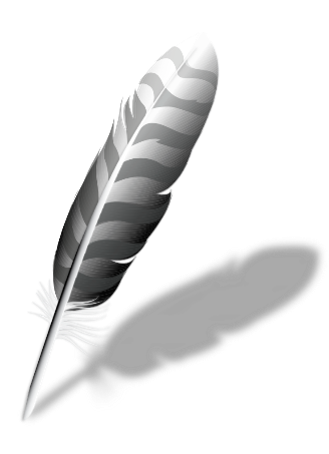
\includegraphics[width=30mm, height=30mm]{assets/imgs/methodology/tkinter_logo.png}}

    \citep{cite_tkinter_official}
    
    &
    
    Tkinter is a built-in Python library. It has a simple learning curve and is compatible with most Python programs. It is also open-source and there are external APIs that make the designs easier.
    
    &
    
    It is not compatible (out-of-the-box) with mobile devices. It does not give a simple solution for multi-interface programs.
    
    \\ \hline
    \end{tabular}
\caption{\label{tab:tkinter} Tkinter solution alternative.}
\end{center}
\end{table}


\begin{table}[H]
\begin{center}
    \begin{tabular}{M{6.6cm}M{3.3cm}M{3.3cm}}
    \hline
    \rowcolor[HTML]{C0C0C0} 
    \textbf{Solution Alternative} & \textbf{Advantages} & \textbf{Disadvantages} \\ 
    \hline

    \textbf{Bash Terminal}
    
    \raisebox{-\totalheight}{
\includegraphics[width=35mm, height=25mm]{assets/imgs/methodology/bash_teminal_logo.png}}

    \citep{cite_bash_terminal}
    
    &
    
    It is the fastest possible solution for sending commands to interact with the system. It gives more possibilities for sending commands with different variables and scripts.
    
    &
    
    There are more possibilities of sending wrong commands, wrong parameters and errors. It is not friendly for the interaction. A great technical knowledge is needed for its usage.
    
    \\ \hline
    \end{tabular}
\caption{\label{tab:bash} Bash solution alternative.}
\end{center}
\end{table}

\begin{table}[H]
\begin{center}
    \begin{tabular}{M{6.6cm}M{3.3cm}M{3.3cm}}
    \hline
    \rowcolor[HTML]{C0C0C0} 
    \textbf{Solution Alternative} & \textbf{Advantages} & \textbf{Disadvantages} \\ 
    \hline

    \textbf{ElectronJs}
    
    \raisebox{-\totalheight}{
\includegraphics[width=30mm, height=30mm]{assets/imgs/methodology/electron_js_logo.png}}

    \citep{cite_electron_js}
    
    &
    
    It is a Graphical User Design tool that makes it simple to create interactive and pretty desktop applications. It has a high-performance interaction and a reusable framework.
    
    &
    
    It is normally a slow-start/slow-running program. It requires high amount of resources in the execution. It requires necessarily a web-server.
    
    \\ \hline
    \end{tabular}
\caption{\label{tab:electronjs} ElectronJs solution alternative.}
\end{center}
\end{table}


\subsubsection{Execute control algorithm for achieving current task}

In order to deliver correctly the food to the user, the system must be able to track and move its structure to the final mouth position in a dynamic and secure way.\\

The following alternatives, are different general control strategies that govern real solutions for different applications. There will be a comparison to determine which one adapts better for the feeding problem.\\


\begin{table}[H]
\begin{center}
    \begin{tabular}{M{6.6cm}M{3.3cm}M{3.3cm}}
    \hline
    \rowcolor[HTML]{C0C0C0} 
    \textbf{Solution Alternative} & \textbf{Advantages} & \textbf{Disadvantages} \\ 
    \hline
    
    \textbf{PID}

    \raisebox{-\totalheight}{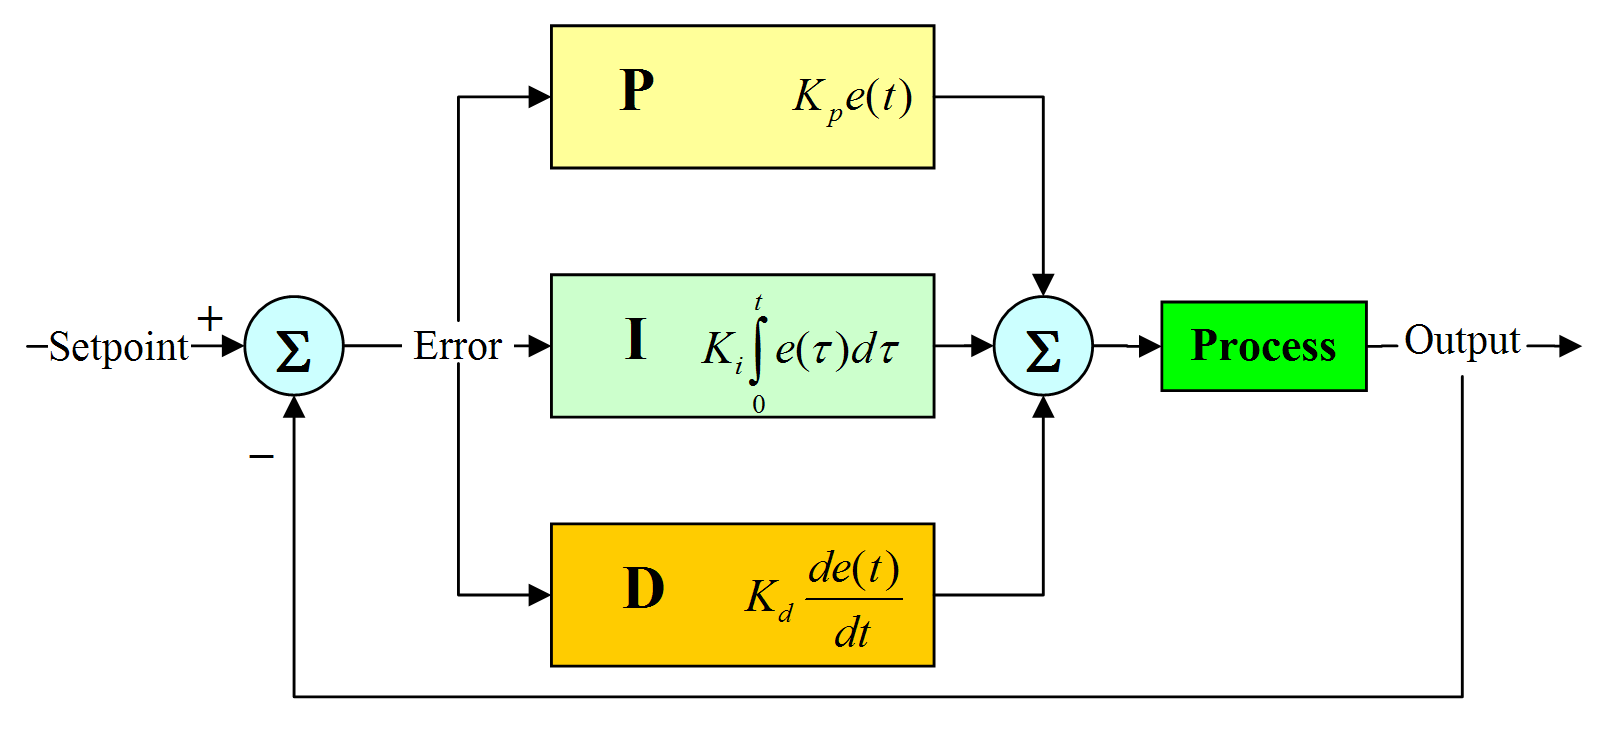
\includegraphics[width=65mm, height=25mm]{assets/imgs/methodology/pid_control.png}}
    
    \citep{cite_PID_control}
    
    &
    
    It is a well-known control strategy with multiple examples, documentation and real-life controllers ready-to-go. It is easy to implement.
    
    &
    
    They have poor control performances for an integrating process and a large time delay process. Hard to incorporate ramp-type set-point change or slow disturbance conditions.
    
    \\ \hline
    \end{tabular}
\caption{\label{tab:pid} PID solution alternative.}
\end{center}
\end{table}

\begin{table}[H]
\begin{center}
    \begin{tabular}{M{6.6cm}M{3.3cm}M{3.3cm}}
    \hline
    \rowcolor[HTML]{C0C0C0} 
    \textbf{Solution Alternative} & \textbf{Advantages} & \textbf{Disadvantages} \\ 
    \hline
    
    \textbf{IMC}

    \raisebox{-\totalheight}{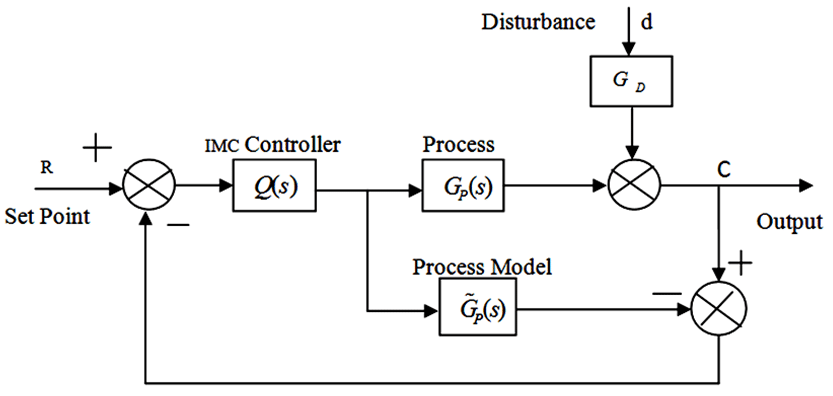
\includegraphics[width=65mm, height=25mm]{assets/imgs/methodology/imc_control.png}}
    
    \citep{cite_IMC_control}
    
    &
    
    It is a control strategy extremely simple to implement. It also has a condition that makes it possible to add extensions for MIMO systems as well as for some nonlinear systems straightforward.

    &
    
    It is common that IMC strategies have drawbacks such as a \say{recovery from process disturbances time}  very slow, compared to the system dynamics.
    
    \\ \hline
    \end{tabular}
\caption{\label{tab:imc} IMC solution alternative.}
\end{center}
\end{table}

\begin{table}[H]
\begin{center}
    \begin{tabular}{M{6.6cm}M{3.3cm}M{3.3cm}}
    \hline
    \rowcolor[HTML]{C0C0C0} 
    \textbf{Solution Alternative} & \textbf{Advantages} & \textbf{Disadvantages} \\ 
    \hline
    
    \textbf{MPC}

    \raisebox{-\totalheight}{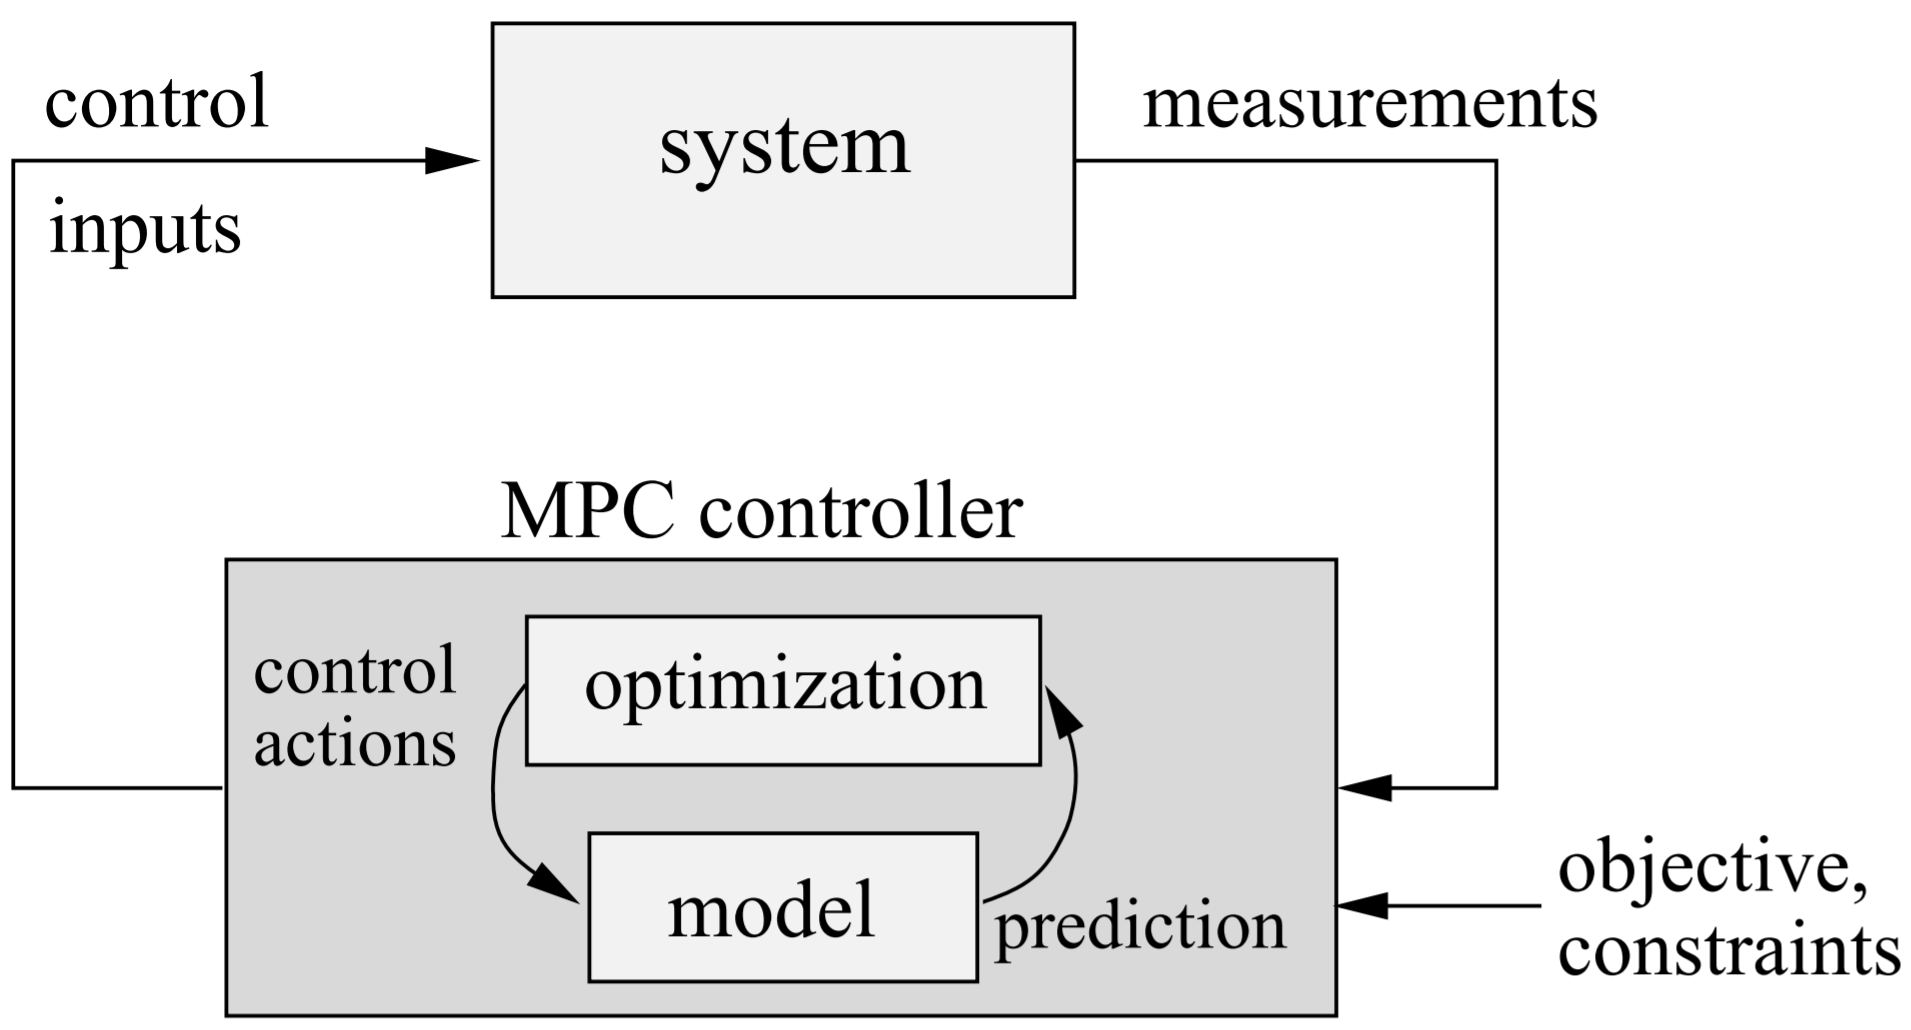
\includegraphics[width=65mm, height=25mm]{assets/imgs/methodology/mpc_control.png}}
    
    \citep{cite_model_predictive_control_camacho_bordons}

    &
    
    It is a flexible control strategy for linear and non-linear systems and/or multi-variable systems. It takes into account the constraints of the system and its variables.

    &
    
    It needs an accurate dynamic model of the system, and a computational algorithm for an optimization problem, that requires high computational cost.
    
    \\ \hline
    \end{tabular}
\caption{\label{tab:mpc} MPC solution alternative.}

\end{center}
\end{table}

\subsubsection{Operate robot}

In order to have a robot structure that is able to give food to the patients, it is necessary to choose a robot that has the right compliance for this activity.\\

The next alternatives, are robots that are available in the \say{Laboratory of Industrial Automation} of the EIA University:\\

\begin{table}[H]
\begin{center}
    \begin{tabular}{M{6.6cm}M{3.3cm}M{3.3cm}}
    \hline
    \rowcolor[HTML]{C0C0C0} 
    \textbf{Solution Alternative} & \textbf{Advantages} & \textbf{Disadvantages} \\ 
    \hline
    
    \textbf{ABB IRB140 Robot}

    \raisebox{-\totalheight}{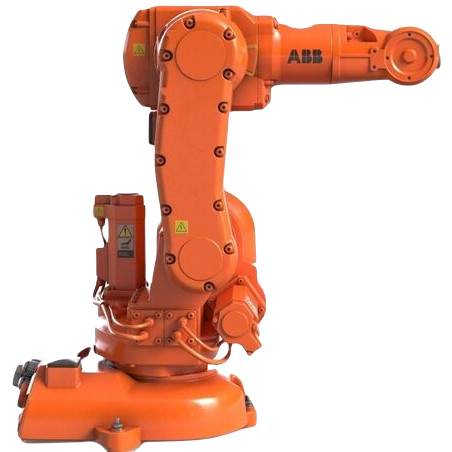
\includegraphics[width=50mm, height=25mm]{assets/imgs/methodology/abb_robot.png}}
    
    \citep{cite_abb_robots}

    &
    
    It has a great documentation and its structures and controllers are easily replaced. It has an excellent support assistance from ABB robotics.
    
    &
    
    It does not have a collaborative approach and is only used for industrial applications. It does not have  have any embedded external sensors for its environment.
    
    \\ \hline
    \end{tabular}
\caption{\label{tab:abb} ABB IRB140 robot solution alternative.}
\end{center}
\end{table}

\begin{table}[H]
\begin{center}
    \begin{tabular}{M{6.6cm}M{3.3cm}M{3.3cm}}
    \hline
    \rowcolor[HTML]{C0C0C0} 
    \textbf{Solution Alternative} & \textbf{Advantages} & \textbf{Disadvantages} \\ 
    \hline
    
    \textbf{Baxter Robot}

    \raisebox{-\totalheight}{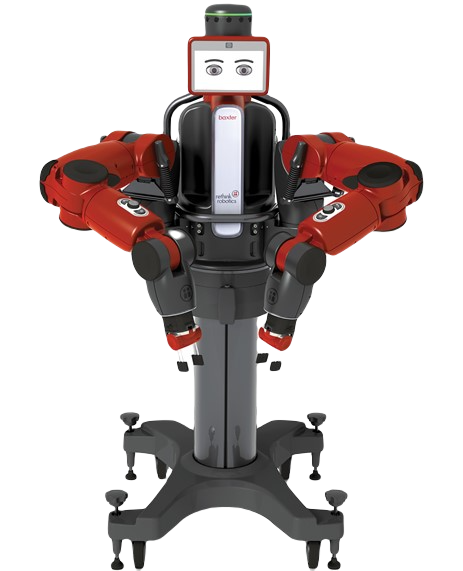
\includegraphics[width=40mm, height=55mm]{assets/imgs/methodology/baxter_robot.png}}
    
    \citep{cite_rethink_robotics_baxter_factory_worker}

    &

    It is a collaborative robot designed for interaction with people and its environment. It has a ROS open-source system interconnected with multiple sensors.

    &

    It does not have external support by the manufacturer (Rethink Robotics). Its operating system runs in  software from 2015.

    \\ \hline
    \end{tabular}
\caption{\label{tab:baxter} Baxter robot solution alternative.}
\end{center}
\end{table}

\subsubsection{Execute computer vision algorithms}

One fundamental step in the process of giving food to the user, is detecting where his mouth is located in an accurate way and in a real-time approach.\\

To correctly implement this condition, the system must have a great camera that is able to capture the user's face and then, send this information to a computer vision algorithm that makes it possible to detect the mouth.\\

The considered alternatives for the vision sub-system cameras are:\\


\begin{table}[H]
\begin{center}
    \begin{tabular}{M{6.6cm}M{3.3cm}M{3.3cm}}
    \hline
    \rowcolor[HTML]{C0C0C0} 
    \textbf{Solution Alternative} & \textbf{Advantages} & \textbf{Disadvantages} \\ 
    \hline
    
    \textbf{Stereo Camera}

    \raisebox{-\totalheight}{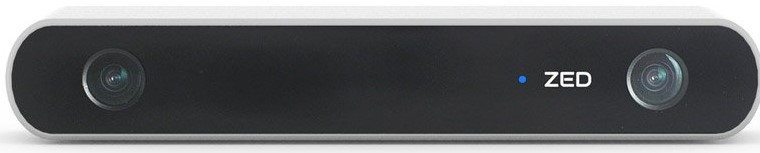
\includegraphics[width=50mm, height=12mm]{assets/imgs/methodology/stereo_camera.png}}
    
    \citep{cite_stereo_camera_zed}

    &
    
    It is able to detect the depth of the image with its two cameras placed similarly to a human-vision-condition.
    
    &
    
    It requires high computational resources and constant calibration for the depth algorithms. Usually are more expensive than other cameras.
    
    \\ \hline
    \end{tabular}
\caption{\label{tab:stereo} Stereo camera solution alternative.}
\end{center}
\end{table}

\begin{table}[H]
\begin{center}
    \begin{tabular}{M{6.6cm}M{3.3cm}M{3.3cm}}
    \hline
    \rowcolor[HTML]{C0C0C0} 
    \textbf{Solution Alternative} & \textbf{Advantages} & \textbf{Disadvantages} \\ 
    \hline
    
    \textbf{Baxter hand cameras}

    \raisebox{-\totalheight}{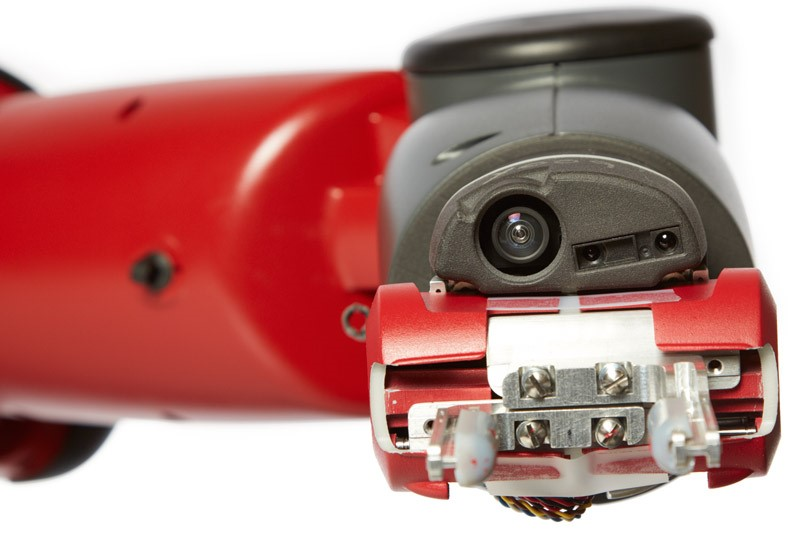
\includegraphics[width=50mm, height=40mm]{assets/imgs/methodology/baxter_hand_camera.jpg}}
    
    \citep{cite_baxter_hand_camera}

    &

    It is integrated with Baxter ROS signals and has the commands already implemented. The cameras are already calibrated and there are examples of its usage. Does not require any external structure or design.

    &

    It does not have depth considered in the information given by the cameras. Is not easily replaced if it is damaged.

    \\ \hline
    \end{tabular}
\caption{\label{tab:baxter_hand_camera} Baxter hand cameras solution alternative.}
\end{center}
\end{table}

\begin{table}[H]
\begin{center}
    \begin{tabular}{M{6.6cm}M{3.3cm}M{3.3cm}}
    \hline
    \rowcolor[HTML]{C0C0C0} 
    \textbf{Solution Alternative} & \textbf{Advantages} & \textbf{Disadvantages} \\ 
    \hline
    
    \textbf{RGBD Camera}

    \raisebox{-\totalheight}{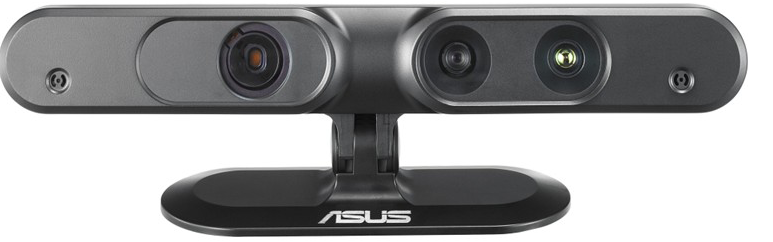
\includegraphics[width=50mm, height=12mm]{assets/imgs/methodology/rgbd_camera.png}}
    
    \citep{cite_rgbd_camera}

    &

    It is able to detect the depth of the image with its infra-red embedded projector with a low cost price. Multiple algorithms for SLAM applications. The community and online support is excellent.

    &

    It requires high computational resources. The depth is limited because sensors only allow measurement ranges of a limited distance and a limited field of view

    \\ \hline
    \end{tabular}
\caption{\label{tab:rgbd} RGB-D cameras solution alternative.}
\end{center}
\end{table}

\subsection{Morphological matrix result}

After diving into each alternative for the overall solution, the result morphological matrix for the autonomous robot feeding problem is the following:


\begin{center}
\includegraphics[width= 1.01\textwidth]{\string "assets/pdfs/methodology/morphological_matrix".pdf}
\bigbreak
\begin{minipage}{\linewidth} %Keep image/PDF in only 1 page
\captionof{figure}{Morphological matrix for the possible concepts A, B and C. Own work.}\label{fig_general_morphological_matrix}
\end{minipage} \end{center}


\section{PUGH Decision matrix}

After the development of the morphological matrix, it is mandatory select the best possible solution based on a quantitative qualification approach. There are multiple ways to discern into the most recommended solution, and for this article, it will be chosen with the help of the \say{PUGH Decision Matrix} (PM) \citep{cite_pugh_matrix}.\\

The PUGH matrix, compares the concepts in a objective-like ways, to determine a possible heuristic solution to the problem based on the engineering conditions defined in the HoQ of the methodology (the ones that impact directly to the user requirements). This decision matrix is considered a great approach, because it involves the most important part of the design, which is what the user really needs.\\

The result of the PUGH matrix for the assistive robotic feeding is:\\

\begin{table}[H]
\begin{center}
    \begin{tabular}{|c|c|c|c|c|c|}
    \hline
    \rowcolor[HTML]{C0C0C0} 
    \multicolumn{3}{|c|}{\cellcolor[HTML]{C0C0C0}\textbf{Concepts}}                               & \textbf{1} & \textbf{2}  & \textbf{3}  \\ \hline
    \rowcolor[HTML]{C0C0C0} 
    \multicolumn{3}{|c|}{\cellcolor[HTML]{C0C0C0}\textbf{Name of concept}}                        & \textbf{A} & \textbf{B}  & \textbf{C}  \\ \hline
    \cellcolor[HTML]{C0C0C0}                   & \textbf{1} & Robot's memory                      & =          & -           & =           \\ \cline{2-6} 
    \cellcolor[HTML]{C0C0C0}                   & \textbf{2} & Robot's processor                   & =          & -           & =           \\ \cline{2-6} 
    \cellcolor[HTML]{C0C0C0}                   & \textbf{3} & Robot's hard drive                  & =          & -           & =           \\ \cline{2-6} 
    \cellcolor[HTML]{C0C0C0}                   & \textbf{4} & Robot's accuracy for joint encoders & =          & =           & =           \\ \cline{2-6} 
    \cellcolor[HTML]{C0C0C0}                   & \textbf{5} & Robot's max payload                 & =          & +           & =           \\ \cline{2-6} 
    \cellcolor[HTML]{C0C0C0}                   & \textbf{6} & Cameras resolution                  & =          & +           & =           \\ \cline{2-6} 
    \cellcolor[HTML]{C0C0C0}                   & \textbf{7} & Cameras focal length                & =          & =           & -           \\ \cline{2-6} 
    \multirow{-8}{*}{\cellcolor[HTML]{C0C0C0}} & \textbf{8} & Cameras frame rate                  & =          & =           & -           \\ \hline
    \multicolumn{3}{|c|}{\cellcolor[HTML]{C0C0C0}\textbf{Sum of the positive signs}}              & 0          & 2           & 0           \\ \hline
    \multicolumn{3}{|c|}{\cellcolor[HTML]{C0C0C0}\textbf{Sum of the negative signs}}              & 0          & 3           & 2           \\ \hline
    \multicolumn{3}{|c|}{\cellcolor[HTML]{C0C0C0}Overall result}                                  & \textbf{0} & \textbf{-1} & \textbf{-2} \\ \hline
    \end{tabular}
\caption{\label{tab:pugh_matrix} PUGH decision matrix for active feeding system}
\end{center}
\end{table}

As it can be seen in the table tab[\ref{tab:pugh_matrix}], the overall result A was the best concept, based on the given engineering conditions for the analysis.\

After evaluating and analyzing the \say{PUGH Decision Matrix}, the result was clearly aiming towards the A concept, which is explained in detail in the solution alternatives section.\\

After this part of the investigation, all of the procedures will be based on the following selected solution alternatives:\\

\begin{enumerate}
    \item Process and send commands through user's interface: Tkinter.
    \item Execute control algorithm for achieving current task: MPC.
    \item Operate robot: Baxter robot.
    \item Execute computer vision algorithms: Baxter hand cameras.
\end{enumerate}


\section{Software architecture}

Although the general system architecture discussed on fig[\ref{fig_general_block_diagram}], enables the understanding of the signals and important information of the complete process workflow, it is extremely valuable to dive into how the software operates in order to achieve these functionalities. In the next diagram, the general software architecture will be presented divided into several layers of abstraction.\\

\begin{center}
\includegraphics[width= 0.8\textwidth]{\string "assets/pdfs/methodology/BaxterSoftwareArchitecture".pdf}
\bigbreak
\begin{minipage}{\linewidth} %Keep image/PDF in only 1 page
\captionof{figure}{General software diagram for system's functionalities. Own work.}\label{fig_general_software_architecture}
\end{minipage} \end{center}


\subsection{Control \& Device Layer}

The control and devices layer has low-level controllers and sensors that will allow to measure the current state of Baxter at all times. This layer has several embedded elements, where some of them can be subtly modified and others are black boxes that can not be edited at a low level operation.\\

In the control layer, it is important to keep in mind that the controllers mentioned are designed for Baxter and have a number of additional protections to prevent damaging them, ensuring that Baxter is a very safe robot and suitable for educational tests.\\


\subsection{Functional Layer}

The functional layer enables the most challenging and complex processing algorithms to be performed throughout the system. This layer is intended to perform the main tasks of the system, allowing control strategies, computer vision algorithms, anomaly detection and, continuous operation guardians for each one of the critical components.\\

The control algorithms will be divided into an MPC for the robot trajectories and an a trajectory planning in order to decide where the end effector should move, achieving a coordination of more than one control algorithm at the same time.\\

There will be a perception subsystem, where the correct detection of the position of the user's mouth and the position of the food will be guaranteed through computer vision algorithms. These will be connected in cascade as feeds for the inputs to the control algorithms.\\

The anomaly detector acts as a \say{supervisory agent} that is constantly receiving signals from the other subsystems and validating non-conventional behaviors in order to stop the system in case of the detection of an anomaly. This should be integrated with a \say{continuous supervisor} that restarts a given system if it detects any strange failure, such as a run-time exception or a memory failure, so the system keeps working normally at every moment.\\

\subsection{Task Layer}

The task layer is in charge of orchestrating each one of the steps of the finite state machine that will allow the dynamic operation of Baxter for each one of the tasks required in the food process (such as, for example, picking up the food and feeding the patient).\\

This finite state machine (FSM), understood as \say{a computation model that can be implemented with hardware or software and can be used to simulate sequential logic and some computer programs} \citep{cite_finite_state_machine_brilliant}, will decide which of the Baxter's tasks will be implemented in the main control algorithms, in order to generate the desired output of the system.\\

The task layer is a fundamental element in the system, because it understands and translates the user's inputs, into states of the FSM, enabling Baxter to move according to the user's needs.\\

This FSM must be designed with a correct architecture for guaranteeing that each state does not fall into an unstable switching condition between two or more tasks.\\

\subsection{User Layer}

This layer works as the highest layer of abstraction, where the user will interact with a simple Graphical User Interface (GUI) and will decide how Baxter should move based on the current state of his meal.\\

The GUI will be developed as a desktop application that connects strategically with the lower-level algorithms developed for the Finite State Machine. It will also have an integrated middle-ware,  that acts as a connector between the subsystems that govern the feeding processes, so that it can take important actions if something wrong happens (like the sudden stop of an specific subsystem).\\

A middle-ware is defined as \say{a software that bridges gaps between other applications, tools, and databases in order to provide unified services to users} \citep{cite_middleware_definition_talend}.\\


\section{Finite State Machine} \label{cite_finite_state_machine_section}

The finite state machine has the purpose of managing the general behaviour of the system in each of the main tasks that Baxter (and the associated subsystems) will perform in the feeding tasks, according to the user's commands.\\

It is important to notice that there are multiple states that have transitions based on a specific condition that changes in the system (for example, a command given by the user). In the next diagram, it will be shown the general structure of the Finite State Machine for the feeding system with its specific transition conditions and states:\\


\begin{center}
\includegraphics[width= 0.9\textwidth]{\string "assets/pdfs/methodology/GeneralFiniteStateMachine".pdf}
\bigbreak
\begin{minipage}{\linewidth} %Keep image/PDF in only 1 page
\captionof{figure}{General software diagram for system's functionalities. Own work.}\label{fig_general_finite_machine}
\end{minipage} \end{center}

\subsection{Shutdown state}

The shutdown state is the default state in which the Baxter robot is completely static, because all of the joint-controllers are turned down. This state is the nearest one to a real hard drive shutdown of the robot, and any trial to transition to another state that is not the \say{Ready State}, will end up in nothing.\\

This state, not only works as an initialization condition, but also determines a safety state in which the robot behaviour can be completely stopped, similarly to the emergency physical button that Baxter has.\\

It is important to notice that any other state of the system, is able to change directly and immediately to the \say{Shutdown State}. This was designed thinking about the importance of the safety of the patients.\\

\subsection{Ready State}

As its name implies, the \say{Ready State} is the one that enables the whole system and prepares it to start working correctly. The transition to this state is only possible with the \say{Start Button} transition.\\

When the user starts the system, it is a condition that should enable the robot's controllers and it runs the important initialization programs for all the sub-systems algorithms and run-time routines.\\

\subsection{Neutral State}

This state is considered to be one of the central and most used states for the overall functionalities. This state should prepare the robot to start the movements of any other state conditions, such as \say{Pick Up Food}, \say{Give Food} and \say{Shutdown}.\\

The neutral state is popularly known as the \say{Home Condition}, because is a well known workspace disposition for the robot environment and conditions of its degrees of freedom for the limbs.\\

It is also important to notice that every other movement state, usually ends up in the \say{Neutral State}, which means that this state is a logical connector between each one of the tasks of the system.\\

\subsection{Food Scooping States}

The \say{Food Scooping States} are composed of the \say{Move to default food position state} and the \say{Scoop food state}. These states work together as a complete task of food scooping, and will always be executed in series, starting by the first one.\\

It is important to realize, that there is no default transition condition to go to the \say{Neutral State}, which implies that at the end of the execution of the tasks of this state, the system will automatically return to home by its own algorithm.\\

Both states of the \say{Food Scooping States}, will be able to stop their procedure, when the user executes a shutdown transition. This will cancel the tasks and return the system to the \say{Shutdown State}.\\


\subsection{Feeding States}

The \say{Feeding States} are designed with three main internal states. These are:\\

\begin{enumerate}
    \item Detect user's mouth state.
    \item Move close to the user's mouth state.
    \item Wait for user's command to return home state.
\end{enumerate}

After analysing the structure and transitions of these internal states, it is clear that there is an internal control loop as a result of the first two states. This control loop is a logical consequence of the need of a feedback-wise system that interacts dynamically with the environment and the patient.\\

At the end of the \say{Feeding States}, the user can decide to stop the system or to return to the neutral state. This decision will also direction the finite state machine, to prepare the system for a future command (such as \say{Food Scoping State}, \say{Feeding States}, or, a final \say{Shutdown State}).\\

\subsection{Stop State}

As mentioned before, the \say{Stop State} is a condition that guarantees that the robot does not move or execute any motion command. This pause is a software condition that does not mean that the controllers are off, instead of that, this state works based on a series of conditions and regulations that stop the robot in a safe way.\\


\section{Important Project Remarks}

This research project will be designed implementing an active robotic solution with Baxter cobot. There are some important concepts to understand for the reach of this investigation.\\

The first key condition, is that the project will be named \say{Baxter Bon Appetit}, referring to the french common expression that has the objective of positively implying someone to enjoy their meal. The purpose of this name, is to create an etymological meaning that transcends in an outstanding robotic solution, that generates a safety feeling of appreciating a good meal.\\

\begin{figure}[H]
    \centering
    
\includegraphics[width=0.7\linewidth]{assets/imgs/methodology/baxter_bon_appetit_logo.png}
    \caption{Baxter Bon Appetit project logo. Own development.} 
    \label{fig_baxter_bon_appetit_logo}
\end{figure}

Another valuable appreciation, is that the initial experiments of this research project, will be tested on the authors (Santiago Garcia Arango and Elkin Javier Guerra Galeano), but for future improvements, there will be a greater development of quality assurance tests in multiple patients. This will be discussed in the \say{Ethical Considerations} on the final chapters.\\


% ---------------------------------------------------------

\chapter{Baxter Robot}

The robot that will be implemented in this research is the Baxter robot from Rethink Robotics (founded by Rodney Brooks)\citep{cite_baxter_main_wiki}. Baxter cobot is a collaborative robot with two arms and an interactive head. This robot has a series of tools and internal safety systems that makes it possible to develop robotic solutions at the industrial and academic levels.\\

\begin{figure}[H]
    \centering
    \includegraphics[width=0.8\linewidth]{assets/imgs/baxter_robot/baxter_general_photo_us.png}
    \caption{General view of Baxter Robot. Taken at the EIA University Laboratory} 
    \label{fig_baxter_general_photo_us}
\end{figure}

\section{Baxter Robot Discovery and Characterization}

To work with Baxter robot, it is important to refer to the official Baxter Rethink Robotics Wiki. This website has multiple valuable features and information about the setup, functionalities, SDKs, considerations and development of solutions with Baxter \citep{cite_baxter_main_wiki}.\\

To dive into the official documentation of Baxter robot, please refer to:

\begin{itemize}
    \color{blue}
    \item \href{https://sdk.rethinkrobotics.com/wiki/Home}{Baxter Rethink Robotics Wiki}
\end{itemize}

In this section, it will be discussed some important aspects of Baxter's initial discovery and characterization for the research work.\\

\subsection{Baxter Initial Setup}

To correctly configure Baxter for the first time, it is important to refer to the \say{Initial Setup} tutorials. These tutorials can be found at:

\begin{itemize}
    \color{blue}
    \item \href{https://sdk.rethinkrobotics.com/wiki/Getting_Started}{Baxter Initial Setup}
\end{itemize}

For the development of this research project, Baxter was already assembled with its pedestal and physical connections already plugged in.\\

The first steps to configure and check Baxter right performance, was to connect a physical keyboard to Baxter's back USB connector. This connections was done in the back of Baxter with the USB entry as can be seen in fig[\ref{fig_baxter_back_part_closeup}]:\\


\begin{figure}[H]
    \centering
    \includegraphics[width=0.6\linewidth]{assets/imgs/baxter_robot/baxter_back_connections_zoom_labeled.jpg}
    \caption{Back view of Baxter robot. Taken at the EIA University Laboratory} 
    \label{fig_baxter_back_part_closeup}
\end{figure}


After that connection, we ran a pre-boot configuration to validate low-level hardware checks to confirm that each one of Baxter components was working correctly. The tests passed successfully in the validation.\\

\begin{figure}[H]
    \centering
    \includegraphics[width=0.6\linewidth]{assets/imgs/baxter_robot/baxter_calibration_setup.png}
    \caption{Implementation of low-level hardware checks in the FSM menu. Taken at the EIA University Laboratory} 
    \label{fig_low_level_checks_fsm}
\end{figure}


As well as the hardware checks, the official documentation implies that it is important to run Baxter joint-controller calibrations every month \citep{cite_baxter_arms_calibartion}. This process is relevant in order to guarantee that the robot's arms responding reliable on its movements and on its specific sensor signals.\\

This calibration was implemented with an internal Baxter ROS node that ran a programmatic routine for about 30 minutes. The step-by-step documentations are found in this wiki:

\begin{itemize}
    \color{blue}
    \item \href{https://sdk.rethinkrobotics.com/wiki/Arm_Calibration}{Baxter Arm Calibration}
\end{itemize}

After this initial configurations, it was concluded that Baxter general low-level conditions and controller calibrations were working perfectly.\\


\subsection{Baxter Components Specifications}

It is mandatory to have a clear and descent understanding of Baxter components. This knowledge can help to determine the way in which the robotic solutions are developed and optimized. A robotic system is usually assembled with default general parts, such as arm(s), end tools, sensor and security components. In this section, Baxter components will be examined in a general point of view.\\

The main Baxter components are:

\subsubsubsection{Robot}

As clear as it could be seen, Baxter robot has a central computer unit that is located inside of its torso. This
CPU is able to run multi thread programs to perform complex robotic operations that involve multiple applications.\\

It is also important to specify that the most important interactive safety measure is known as the \say{Emergency Button}. This E-Button is able to completely shutdown Baxter robot and kill all the underlying processes that are being executed at any time. This acts similarly as an \say{Enable/Disable} condition.\\


\subsubsubsection{Grippers}

Grippers, also known as end effectors, are the final part of a robotic arm. The grippers act as a crucial part of a robot because they enable the manipulation of external elements in a workspace.\\

Baxter robot supports two default type of pre-built grippers. These are: electric grippers and suction grippers. Many applications require one of these end effectors as a primary tool for the correct development of an automation task.\\

Baxter robot, also allows external \say{own-made} grippers to be attached to its hands, making it possible to design multiple solutions that are not initially considered.\\

\subsubsubsection{Head}

Baxter head is a subtle but fundamental component of the robot, because it can be used as an interactive tool to display friendly images and show possible tasks to the user. The head is also a way to demonstrate that Baxter is designed for collaborative environments that are easily adapted to multiple scenarios with people around him.\\ 

The head is also capable of panning a total of 180\textdegree \space in horizontal directions and nodding vertically as well. This condition is a way to implement an extra layer of interactions with the work-space's users.\\

\subsubsubsection{Screen}

The screen is a 1024 x 600 SVGA LCD display that is completely integrated with Baxter internal components. This screen is intended to be an extension of the robot's functionalities.\\

\subsubsubsection{Arms}

One of the particularities of Baxter robot, is that is has two independent arms (which is different than most industrial robots that only have one). The fact that Baxter was developed in this way, is a design strategy to show that the robot is a \say{friendly system} that looks similar to human being, increasing the trust that users have for it.\\

Each arm is composed of seven degrees of freedom that are moved, controlled and measured with internal electro-mechanical components. These arms are also conceived to have multiple \say{Series Elastic Actuators (SEAs)}, that enhance different available control modes, to ensure the overall safety of the system \citep{cite_baxter_arms_wiki}.\\

Baxter hands also implement extra signals sensors, such as cameras, infrared sensors, accelerometers and navigators. These sensors are totally integrated with the internal electronic and software architecture of the system.\\


\subsubsubsection{Cameras}

A key component of the whole system is the fact that it has multiple high-resolution cameras. These cameras are named the \say{left\_hand\_camera}, \say{right\_hand\_camera} and \say{head\_camera}. All cameras are internally connected with Baxter software architecture and enable extra processes such as computer vision algorithms based on the analyzed images.\\

One important limitation to keep in mind is that the hardware conditions do not allow Baxter to operate more than two cameras at the same time (this is because of an internal USB hardware requirement).\\

Baxter also allows to individually configure camera conditions, i.e, window width, window height and max frame rate.\\


\subsubsubsection{Input and Output}

Although the other components may have internal I/O systems, Rethink Robotics considered the \say{Input/Output} conditions as a key feature of the final solution. These I/O are the direct conditions to interact with Baxter robot, and are designed in a robust, secure and easy-to-program way.\\

The three main I/O categories are \say{Analog I/Os}, \say{
Digital I/Os} and \say{Navigator Interface I/Os} \citep{cite_baxter_io_wiki}. All three have different electronic signal behaviours and are composed of: sensors, buttons, switches, lights, then navigators, then digitals and analog IOs.\\


\subsection{Baxter Hardware Specifications}

Baxter robot is documented officially in the Rethink Robotics Wiki with multiple measurements and information about its hardware components.\\

As it is said in the robot's data-sheet, Baxter was designed for continuous operation and can run 24/7 for expended periods of time without the risk of damaging the hardware of the robot\citep{cite_baxter_hardware_specifications}. \\

In this section, we will dive into important characteristics and features that are going to be essential in the future chapters. All of these measurements are taken from the official documentation and were guarantee to have minor errors.\\

\subsubsection{Baxter Arm Specifications}

Both Baxter arms are exactly the same in terms of distances, angles and internal conditions, with the only exception of being symmetrical.\\

In the following image (fig[\ref{fig_baxter_hand_measurements}]), there is a detailed explanation of Baxter hand with the notation of its angle names (that are used for the internal processing and execution of Baxter commands):

\begin{figure}[H]
    \centering
    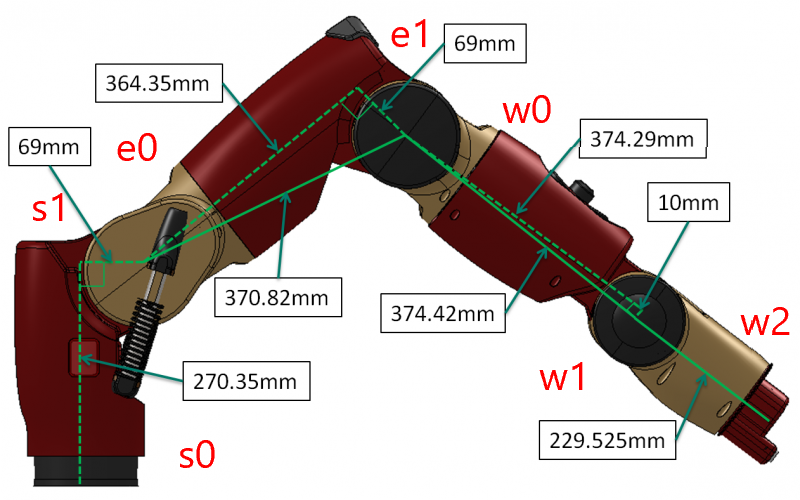
\includegraphics[width=0.7\linewidth]{assets/imgs/baxter_robot/baxter_arm_specifications.png}
    \caption{Hand measurements and angle names for Baxter robot. Adapted from \citep{cite_baxter_hardware_specifications}.} 
    \label{fig_baxter_hand_measurements}
\end{figure}


\begin{table}[H]
\begin{center}
\scalebox{0.81}{
    \centering
    \begin{tabular}{|c|c|c|c|c|c|c|}
    \hline
    \rowcolor[HTML]{C0C0C0} 
        \textbf{Joint} & \textbf{(Degrees) Min limit} & \textbf{Max limit} & \textbf{Range} & \textbf{(Radians) Min limit} & \textbf{Max limit} & \textbf{Range} \\ \hline
        S0 & -97.494 & +97.494 & 194.998 & -1.7016 & +1.7016 & 3.4033 \\ \hline
        S1 & -123 & +60 & 183 & -2.147 & +1.047 & 3.194 \\ \hline
        E0 & -174.987 & +174.987 & 349.979 & -3.0541 & +3.0541 & 6.1083 \\ \hline
        E1 & -2.864 & +150 & 153 & -0.05 & +2.618 & 2.67 \\ \hline
        W0 & -175.25 & +175.25 & 350.5 & -3.059 & +3.059 & 6.117 \\ \hline
        W1 & -90 & +120 & 210 & -1.5707 & +2.094 & 3.6647 \\ \hline
        W2 & -175.25 & +175.25 & 350.5 & -3.059 & +3.059 & 6.117 \\ \hline
    \end{tabular}
}
\caption{\label{tab:max_min_values} Joint range values for Baxter Robot. Adapted from \citep{cite_baxter_hardware_specifications}.}
\end{center}
\end{table}

Another interesting condition that is required for implementing control solutions is the torque and speed of the arms. In the following chart, those conditions are going to be shown.\\


\begin{table}[H]
\begin{center}
\scalebox{1.0}{
    \centering
    \begin{tabular}{|c|c|c|}
    \hline
    \rowcolor[HTML]{C0C0C0} 
        \textbf{Joint} & \textbf{Maximum Speed (rad/sec)} & \textbf{Peak Torque (Nm)} \\ \hline
        S0 & 2.0 & 50 \\ \hline
        S1 & 2.0 & 50 \\ \hline
        E0 & 2.0 & 50 \\ \hline
        E1 & 2.0 & 50 \\ \hline
        W0 & 4.0 & 15 \\ \hline
        W1 & 4.0 & 15 \\ \hline
        W2 & 4.0 & 15 \\ \hline
    \end{tabular}
}
\caption{\label{tab:max_joint_conditions} Maximum joint speed values and torques for Baxter robot. Adapted from \citep{cite_baxter_hardware_specifications}.}
\end{center}
\end{table}


These joint speed values and torques are considered to be fast, considering the normal operating conditions of collaborative robots.\\

To correctly acquire Baxter current joint angles, Baxter has high quality sensor at each on of its degrees of freedom. These sensors have the following specifications:

\begin{itemize}
    \item The resolution for the joint sensors is 14 bits (over 360 degrees); so 360/(2\^14) = 0.021972656 degrees per tick resolution.
    \item The joints have a waveform non-linearity, based on an accuracy on the order of about +/-0.10 degrees, worst case +/-0.25 degrees accuracy when reaching the joint limits.
\end{itemize}

\subsubsection{Baxter Camera Specifications}

Camera signals play a fundamental role in the development of autonomous solutions. For Baxter robot, these conditions are similar for each on of the cameras and are the typical values are the following:

\begin{table}[H]
\begin{center}
\scalebox{1.0}{
    \centering
    \begin{tabular}{|c|c|c|}
    \hline
    \rowcolor[HTML]{C0C0C0} 
        \textbf{Description} & \textbf{Spec} & \textbf{Unit} \\ \hline
        Max Resolution & 1280 x 800 & pixels \\ \hline
        Effective Resolution & 640 x 400 & pixels \\ \hline
        Frame Rate & 30 & frames per second \\ \hline
        Focal Length & 1.2 & mm \\ \hline
    \end{tabular}
}
\caption{\label{tab:camera_specifications} Camera specifications for Baxter robot. Adapted from \citep{cite_baxter_hardware_specifications}.}
\end{center}
\end{table}

It is important to notice that these conditions will be analyzed better in the computer vision algorithms developed in the final sections of this research.\\


\subsubsection{Baxter CPU Specifications}

CPU specifications are a direct limitation for any robotic solution, because the processor is in charge of executing multiple complex threads for the correct real-time applications.\\

\begin{table}[H]
\begin{center}
\scalebox{0.9}{
    \centering
    \begin{tabular}{|c|c|}
    \hline
    \rowcolor[HTML]{C0C0C0} 
        \textbf{Description} & \textbf{Spec} \\ \hline
        Processor & 3rd Gen Intel Core i7-3770 Processor (8MB, 3.4GHz) w/HD4000 Graphics \\ \hline
        Memory & 4GB, NON-ECC, 1600MHZ DDR3 \\ \hline
        Hard Drive & 128GB Solid State Drive \\ \hline
    \end{tabular}
}
\caption{\label{tab:cpu_specifications} CPU specifications for Baxter robot. Adapted from \citep{cite_baxter_hardware_specifications}.}
\end{center}
\end{table}


\subsubsection{Baxter Additional Specifications}

There are some final additional important specifications that Rethink Robotics has considered as relevant to consider in order to develop disruptive robotic solutions. These considerations are specified in table[\ref{tab:additional_specifications}]:

\begin{table}[H]
\begin{center}
\scalebox{0.82}{
    \centering
    \begin{tabular}{|c|c|}
    \hline
    \rowcolor[HTML]{C0C0C0} 
        \textbf{Description} & \textbf{Spec} \\ \hline
        Battery Operation & DC-to-120V AC Inverter \\ \hline
        Max Consumption & 6A at 120V AC, 720W max per unit \\ \hline
        Total weight (with pedestal) & 298 lbs / 135.2 kg \\ \hline
        Screen Resolution & 1024 x 600 pixels \\ \hline
        Positional Accuracy & +/- 5 mm \\ \hline
        Max Payload (including end-effector) & 5 lb / 2.2 kg \\ \hline
        Infrared Sensor Range & 1.5 – 15 in / 4 – 40 cm \\ \hline
    \end{tabular}
}
\caption{\label{tab:additional_specifications} Additional specifications for Baxter robot. Adapted from \citep{cite_baxter_hardware_specifications}.}
\end{center}
\end{table}


\subsection{Baxter Software Specifications}

Robots are devices that must integrate multiple sensors, actuators, protocols, validations, security features, programmable processes and more. This requirements are only possible with the right software and hardware integration for the desired robot features. Based on this statement, there must be an overall layer of abstraction for controlling the specified aspects and executing the robot´s functionalities in a reliable way. For Baxter robot, this software and hardware conditions are run on based on a \say{Robot Operating System} (ROS) \citep{cite_ROS_official_site}.

Baxter runs on ROS Indigo and implements an Ubuntu 14.04 Linux distribution. This software requirements can be eventually upgraded to newer versions with minor work, but is not a straight-forward approach, because some important functionalities could get unstable or not compatible. For this reason, for this research these software requirements are going to be used.\\

\begin{figure}[H]
	\centering
	\begin{subfigure}{.5\textwidth}
		\centering
		
\includegraphics[width=0.7\linewidth]{assets/imgs/baxter_robot/ros_indigo.png}
		\caption{ROS Indigo Igloo implemented in Baxter robot. Taken from \citep{cite_ros_indigo_main_page}}
		\label{fig_ros_indigo_logo}
	\end{subfigure}~
	\begin{subfigure}{.5\textwidth}
		\centering
		
\includegraphics[width=0.55\linewidth]{assets/imgs/baxter_robot/ubuntu_logo.jpg}
		\caption{Ubuntu 14.04 Linux distribution implemented in Baxter robot. Taken from \citep{cite_ubuntu_download_1404}}
		\label{fig_ubuntu_1404_logo}
	\end{subfigure}%
	\caption{Required software dependencies for running Baxter robot.}
	\label{fig_required_baxter_software}
\end{figure}


\section{Baxter Robot Mathematical Approach}

The mathematical approach of any dynamic system, has its foundations on reference frames that enable the absolute and relative Cartesian systems. For robotic systems, it is common to define a main workspace reference and start developing models to transform these coordinates into multiple other references throughout the system.\\

Baxter is a completely symmetrical two armed hyper-redundant 7DOF humanoid robot. This condition makes it useful to define a central reference as the workspace center, so that the transforms are similar in each one of the arms. It's also relevant to notice that both limbs are exactly the same in measurements and the only key difference the sign of an angle.Each arm has a total of seven degrees of freedom (DOF) of rotational joint type (\textbf{R}).\\

In order to be determine the position and orientation of Baxter end effector in a mathematical way, it is important to understand that Baxter has multiple joint-encoder sensors that are only able to measure the angle of an articulation based on the angle that it makes with respect of the previous one.\\

These encoders are already calibrated and are the main way to map the end effector to the central reference frame. To do this mapping, it is mandatory to have a mathematical representation with Transformation Matrices for each one of the reference frames that are in Baxter's joints.\\

In this section, there are some important values to keep in mind for the mathematical results of the transformation matrices. These values correspond to the distances shown in figures fig[\ref{fig_baxter_schematic_general}], fig[\ref{fig_baxter_schematic_torso_to_arm}] and fig[\ref{fig_baxter_schematic_right_arm}]:

\begin{table}[H]
\begin{center}
\scalebox{0.82}{
    \centering
    \begin{tabular}{|c|c|}
    \hline
    \rowcolor[HTML]{C0C0C0} 
        \textbf{Length} & \textbf{Value (mm)} \\ \hline
        L0 & 270.35 \\ \hline
        L1 & 69.00 \\ \hline
        L2 & 364.35 \\ \hline
        L3 & 69.00 \\ \hline
        L4 & 374.29 \\ \hline
        L5 & 10.00 \\ \hline
        L6 & 368.30 \\ \hline
        L & 278.00 \\ \hline
        h & 64.00 \\ \hline
        H & 1104.00 \\ \hline
    \end{tabular}
}
\caption{\label{tab:lengths_of_baxter} Lengths of Baxter robot. Adapted from \citep{cite_baxter_humanoid_robot_kinematics_ohio}.}
\end{center}
\end{table}

There is an extra consideration for these values, because the final distance \say{L6}, is considered as the distance from the wrist pitch center, to the final part of the end effector. Keep in mind that the current value specifies the distance without any tool attached to it. This distance changes based on the distance of the tool that is implemented on Baxter.\\


\subsection{Baxter Fixed Transformation Matrices}

There are some important transformation matrices that enable the mapping of Baxter arms with respect of the main reference frame (this is from \{W0\} to \{BR\} or from \{W0\} to \{BL\}, as it can be seen in figures fig[\ref{fig_baxter_schematic_general}] and fig[\ref{fig_baxter_schematic_torso_to_arm}]. These transforms are considered \say{fixed}, because they are constant in time. That means that we do not need to implement any addition algorithm to calculate the current values (those calculations are only relevant in the angles for Baxter arms).\\

In the following figures, it is possible to determine the relevant reference frames to do the initial transformation matrices:


\begin{center}
\includegraphics[width= 0.98\textwidth]{\string "assets/pdfs/baxter_robot/general_distance_schematic".pdf}
\bigbreak
\begin{minipage}{\linewidth} %Keep image/PDF in only 1 page
\captionof{figure}{General Baxter schematic with reference frames. Adapted from \citep{cite_baxter_humanoid_robot_kinematics_ohio}.}\label{fig_baxter_schematic_general}
\end{minipage} \end{center}


\begin{center}
\includegraphics[width= 0.9\textwidth]{\string "assets/pdfs/baxter_robot/body_to_shoulder_schematic".pdf}
\bigbreak
\begin{minipage}{\linewidth} %Keep image/PDF in only 1 page
\captionof{figure}{Torso to arm schematic with reference frames. Adapted from \citep{cite_baxter_humanoid_robot_kinematics_ohio}.}\label{fig_baxter_schematic_torso_to_arm}
\end{minipage} \end{center}


The transformation matrices from the central reference, to the beginning of Baxter arms, are:\\

\begin{equ}[H]
\begin{equation} \label{eq:transformation_matrix_w0_bl_and_w0_br}
    \begin{bmatrix}
    _{B_L}^{W_0}\textrm{T}
    \end{bmatrix}
    =
    \begin{bmatrix}
    \frac{\sqrt{2}}{2} & \frac{\sqrt{2}}{2} & 0 & L \\ 
    -\frac{\sqrt{2}}{2} & \frac{\sqrt{2}}{2} & 0 & -h \\ 
    0 & 0 & 1 & H \\ 
    0 & 0 & 0 & 1
    \end{bmatrix}
    \phantom{0000}
    \begin{bmatrix}
    _{B_R}^{W_0}\textrm{T}
    \end{bmatrix}
    =
    \begin{bmatrix}
    -\frac{\sqrt{2}}{2} & \frac{\sqrt{2}}{2} & 0 & -L \\ 
    -\frac{\sqrt{2}}{2} & -\frac{\sqrt{2}}{2} & 0 & -h \\ 
    0 & 0 & 1 & H \\ 
    0 & 0 & 0 & 1
    \end{bmatrix}
\end{equation}
\myequations{Transformation matrices from W0 to BL and from W0 to BR}
\caption{Transformation matrices from W0 to BL and from W0 to BR.}
\end{equ}

These matrices have exactly the same absolute values in terms of the distances, but the only key difference is the sign of the translations and rotations. This difference is due to the fact that the robot is symmetrical and thus, the values are the opposite respect to X-axis in translation and a 90 degree difference in Z-axis the rotation (with respect to each other).\\

After these fixed transformation matrices are taken into consideration, there are two extra constant transformations that must be done before applying the DH parameters algorithm. These transformations are based on the frames specified on fig[\ref{fig_baxter_schematic_right_arm}]:

\begin{itemize}
    \item Transformation from the reference frame of the arm of Baxter (\{BR\} or \{BL\}) to the beginning of the variable part of Baxter's arm (\{0\}).
    \item Transformation from the reference frame of the end of Baxter arm (\{7\}) to the end effector (\{GL\} or \{GR\}).
\end{itemize}

\begin{equ}[H]
\begin{equation} \label{eq:transformation_matrices_fixed_init_of_arm_and_end_of_arm}
    \begin{bmatrix}
    _{0}^{B_L}\textrm{T}
    \end{bmatrix}
    =
    \begin{bmatrix}
    _{0}^{B_R}\textrm{T}
    \end{bmatrix}
    =
    \begin{bmatrix}
    1 & 0 & 0 & 0 \\ 
    0 & 1 & 0 & 0 \\ 
    0 & 0 & 1 & L_0 \\ 
    0 & 0 & 0 & 1
    \end{bmatrix}
    \phantom{0000}
    \begin{bmatrix}
    _{G_L}^{7}\textrm{T}
    \end{bmatrix}
    =
    \begin{bmatrix}
    _{G_R}^{7}\textrm{T}
    \end{bmatrix}
    =
    \begin{bmatrix}
    1 & 0 & 0 & 0 \\ 
    0 & 1 & 0 & 0 \\ 
    0 & 0 & 1 & L_6 \\ 
    0 & 0 & 0 & 1
    \end{bmatrix}
\end{equation}
\myequations{Transformation matrices from BR/BL to 0 and from 7 to GL/GR}
\caption{Transformation matrices from BR/BL to 0 and from 7 to GL/GR.}
\end{equ}


\begin{center}
\includegraphics[width= 0.92\textwidth]{\string "assets/pdfs/baxter_robot/baxter_transformations_explained".pdf}
\bigbreak
\begin{minipage}{\linewidth} %Keep image/PDF in only 1 page
\captionof{figure}{Visual complete transformation matrices for Baxter left hand. Own development.}\label{fig_baxter_transformations_graphic_way}
\end{minipage} \end{center}

After these fixed transformation matrices were explained by inspection, the next section is going to explain how to use the \say{DH notation} to specify how to calculate the missing transformations of the reference frames from \{0\} to \{7\}.\\


\subsection{Baxter Robot Denavit-Hartenberg Parameters}

In robotics, Denavit-Hartenberg Parameters (DH params), are used to specify the relationships and notations of multiple reference frames that are present in a chain-wise robotic system. This algorithm makes it possible to standardize the coordinate frames for spatial linkages easily \citep{cite_denativ_hartenberg}.\\

For Baxter DH Parameters, it is going to be used the modified Denavit-Hartenberg algorithm, also known as the \say{Craig Style DH Params}. This modification only differs in a rotation of frames that happens directly at a joint, instead of a distal joint) \citep{cite_craig_robotics}.\\

\begin{center}
\includegraphics[width= 1.02\textwidth]{\string "assets/pdfs/baxter_robot/right_arm_schematic".pdf}
\bigbreak
\begin{minipage}{\linewidth} %Keep image/PDF in only 1 page
\captionof{figure}{Right arm schematic with reference frames. Adapted from \citep{cite_baxter_humanoid_robot_kinematics_ohio}.}\label{fig_baxter_schematic_right_arm}
\end{minipage} \end{center}

\begin{table}[H]
\begin{center}
\scalebox{0.98}{
    \centering
    \begin{tabular}{|c|c|c|c|c|}
    \hline
    \rowcolor[HTML]{C0C0C0} 
        % \textbf{i} & \textbf{\alpha_{i-1}} & \textbf{a_{i-1}} & \textbf{d_{i}} & \textbf{\theta_{i}} \\ \hline
        $i$ & $\alpha_{i-1}$ & $a_{i-1}$ & $d_{i}$ & $\theta_{i}$ \\ \hline
        1 & 0 & 0 & 0 & $\theta_{1}$ \\ \hline
        2 & -90\textdegree & $L_1$ & 0 & $\theta_{2} + 90$\textdegree \\ \hline
        3 & 90\textdegree & 0 & $L_{2}$ & $\theta_{3}$ \\ \hline
        4 & -90\textdegree & $L_{3}$ & 0 & $\theta_{4}$ \\ \hline
        5 & 90\textdegree & 0 & $L_{4}$ & $\theta_{5}$ \\ \hline
        6 & -90\textdegree & $L_{5}$ & 0 & $\theta_{6}$ \\ \hline
        7 & 90\textdegree & 0 & 0 & $\theta_{7}$ \\ \hline
    \end{tabular}
}
\caption{\label{tab:dh_params} Denavit Hartenberg Parameters for the arms of Baxter robot. Adapted from \citep{cite_denativ_hartenberg}.}
\end{center}
\end{table}

One great advantage of Baxter robot is that the Denavit Hartenberg parameters are identical for both of its arms, making it simple to describe the kinematics and dynamics of the entire system, due to the symmetrical configuration. The main difference will only be considered for the fixed transformation matrices shown in the last section in equations eq[\ref{eq:transformation_matrix_w0_bl_and_w0_br}] and eq[\ref{eq:transformation_matrices_fixed_init_of_arm_and_end_of_arm}].\\

After inspecting and analyzing the Baxter DH parameters table, it is now possible to determine a specific transformation matrix of any of its joints, based on the measurement of the encoder sensors of all of its degrees of freedom. This affirmation will be extremely important, for future calculations that require multiple transformation matrices at a given time.\\ 


\section{Baxter Robot Algorithms}

Two important mathematical algorithms for robot kinematics are the \say{Forward Pose Kinematics} (FPK) and \say{Inverse Pose Kinematics} (IPK). These approaches have different purposes and create the basis of any robotic solution. In FPK, the length of each one of the links and the angles of the DOF are known and the goal is to calculate the position and orientation of the end effector (or any intermediate part) in the physical space of the robot. In the IPK, the length of each one of the links is known and the current position of the end effector is given, and the goal is to calculate the value of the angles for each one of the DOF \citep{cite_fpk_and_ipk_explained_simple}.\\

The FPK and IPK algorithms will be explained in the following sub-sections:

\subsection{Baxter Forward Pose Kinematics}

The objective of the FPK for Baxter, is to determine the position and orientation of the end-effector frame. To solve this problem, we can proceed to implement the DH parameters in the following way:

\begin{enumerate}
    \item Substitute each line of Denavit-Hartenberg Parameters shown in table tab[\ref{tab:dh_params}] with the current joint angle values.
    \item Then, apply the necessary rotations and translations in the DH axes, to determine the intermediate transformation matrices for each one of the links.
    \item Calculate the overall end-effector transformation matrix from the result of matrix multiplication of each one of the intermediate matrices. 
\end{enumerate}

The previous steps can be expressed in a matrix-wise way as it follows (these abbreviations are used: c$\theta_{i}$=cos$\theta_{i}$, s$\theta_{i}$=sin$\theta_{i}$, c$\alpha_{i-1}$=cos$\alpha_{i-1}$, s$\alpha_{i-1}$=sin$\alpha_{i-1}$ ):

\begin{equ}[H]
\begin{equation} \label{eq:transformation_matrices_for_dh_algorithm}
    \begin{bmatrix}
    _{i}^{i-1}\textrm{T}
    \end{bmatrix}
    =
    \begin{bmatrix}
    c\theta_{i} & -s\theta_{i} & 0 & a_{i-1} \\ 
    s\theta_{i}c\alpha_{i-1} & c\theta_{i}c\alpha_{i-1}& -s\alpha_{i-1} & -d_{i}s\alpha_{i-1} \\ 
    s\theta_{i}s\alpha_{i-1} & c\theta_{i}s\alpha_{i-1} & c\alpha_{i-1} & d_{i}c\alpha_{i-1} \\ 
    0 & 0 & 0 & 1
    \end{bmatrix}
    =
    \left[ \begin{array}{ *{4}{c} }
        & & & \\
        & & & \\
        \multicolumn{3}{c}
            {\raisebox{\dimexpr\normalbaselineskip+.5\ht\strutbox-.5\height}[0pt][0pt]
            {\scalebox{1.0}{$_{i}^{i-1}\textrm{R}$}}} & 
            {\raisebox{\dimexpr\normalbaselineskip+.5\ht\strutbox-.5\height}[0pt][0pt]
            {\scalebox{1.0}{$_{}^{i-1}\textrm{P}_i$}}} \\
        0 & 0 & 0 & 1
    \end{array} \right]
\end{equation}
\myequations{Transformation matrices for Denavit Hartenberg algorithm}
\caption{Transformation matrices for Denavit Hartenberg algorithm.}
\end{equ}

The transformation matrices specified in eq[\ref{eq:transformation_matrices_for_dh_algorithm}], correspond to the position and orientation of the desired joint articulation that we want to analyze, and if the final reference frame of Baxter arm is the goal, this transformation matrix would become to the values that go from \{0\} to \{7\}.\\

To obtain the complete matrix transformation from \{0\} to \{7\}, it can apply the properties of homogeneous transformation matrices, like this:

\begin{equ}[H]
\begin{equation} \label{eq:transformation_matrix_from_0_to_7_process}
    \begin{bmatrix}
    _{7}^{0}\textrm{T}
    \end{bmatrix}
    =
    \begin{bmatrix}
    _{1}^{0}\textrm{T}(\theta_{1})
    \end{bmatrix}
    \begin{bmatrix}
    _{2}^{1}\textrm{T}(\theta_{2})
    \end{bmatrix}
    \begin{bmatrix}
    _{3}^{2}\textrm{T}(\theta_{3})
    \end{bmatrix}
    \begin{bmatrix}
    _{4}^{3}\textrm{T}(\theta_{4})
    \end{bmatrix}
    \begin{bmatrix}
    _{5}^{4}\textrm{T}(\theta_{5})
    \end{bmatrix}
    \begin{bmatrix}
    _{6}^{5}\textrm{T}(\theta_{6})
    \end{bmatrix}
    \begin{bmatrix}
    _{7}^{6}\textrm{T}(\theta_{7})
    \end{bmatrix}
\end{equation}
\myequations{Complete Baxter arm transformation matrix from frame \{0\} to frame \{7\} using DH intermediate transforms.}
\caption{Complete Baxter arm transformation matrix from frame \{0\} to frame \{7\} using DH intermediate transforms.}
\end{equ}

As it can be perceived in the transformation matrix obtained in eq[\ref{eq:transformation_matrix_from_0_to_7_process}], it only takes into consideration the frames that change in time, which correspond to the shoulder, wrist and elbow of Baxter arm. However, to apply a complete transform from the defined center of reference \{W0\} to the final end-effector \{GL\} or \{GR\}, the already discussed fixed transformation matrices must be applied correctly.\\

To mathematically express the absolute final position and orientation of the end-effector expressed in homogeneous transformation matrix, the successive expression must be calculated:

\begin{equ}[H]
\begin{equation} \label{eq:transformation_matrix_from_w0_to_GL}
    \begin{bmatrix}
    _{G_L}^{W_0}\textrm{T}
    \end{bmatrix}
    =
    \begin{bmatrix}
    _{B_L}^{W_0}\textrm{T}
    \end{bmatrix}
    \begin{bmatrix}
    _{0}^{B_L}\textrm{T}
    \end{bmatrix}
    \begin{bmatrix}
    _{7}^{0}\textrm{T}
    \end{bmatrix}
    \begin{bmatrix}
    _{G_L}^{7}\textrm{T}
    \end{bmatrix}
\end{equation}
\myequations{Expression to calculate absolute transformation matrix from the reference frame \{W0\} to the left end-effector frame \{GL\}}
\caption{Expression to calculate absolute transformation matrix from the reference frame \{W0\} to the left end-effector frame \{GL\}.}
\end{equ}

\begin{equ}[H]
\begin{equation} \label{eq:transformation_matrix_from_w0_to_GR}
    \begin{bmatrix}
    _{G_R}^{W_0}\textrm{T}
    \end{bmatrix}
    =
    \begin{bmatrix}
    _{B_R}^{W_0}\textrm{T}
    \end{bmatrix}
    \begin{bmatrix}
    _{0}^{B_R}\textrm{T}
    \end{bmatrix}
    \begin{bmatrix}
    _{7}^{0}\textrm{T}
    \end{bmatrix}
    \begin{bmatrix}
    _{G_R}^{7}\textrm{T}
    \end{bmatrix}
\end{equation}
\myequations{Expression to calculate absolute transformation matrix from the reference frame \{W0\} to the right end-effector frame \{GR\}}
\caption{Expression to calculate absolute transformation matrix from the reference frame \{W0\} to the right end-effector frame \{GR\}.}
\end{equ}

An important remark is that for these equations, the only variable matrices are the ones that go from the frames \{0\} to \{7\}, and the value is obtained from the current measurement of the joint encoders angles $\theta_{1}$ to $\theta_{7}$. The other ones were explained before and are constant in time.\\

The software implementation of the FPK algorithm for this research project can be found at our GitHub repository \say{baxter-bon-appetit}:

\begin{itemize}
    \color{blue}
    \item \href{https://github.com/san99tiago/baxter-bon-appetit/blob/main/python/baxter_bon_appetit/src/baxter_essentials/baxter_fpk.py}{Baxter-Bon-Appetit Forward Pose Kinematic Algorithm (Source Code)}
\end{itemize}


\subsection{Baxter Inverse Pose Kinematics} 
\label{sub_sec_ipk}

The goal of the IPK for Baxter, is to determine the current angles of each one of the degrees of freedom, based on the Cartesian position and orientation of the end effector. To solve this problem, we can proceed to derive a general expression based on an analytical solution.\\

One key condition to consider is that Baxter has 7 DOF, which makes him an hyper-redundant robot that can usually get to a given point in space in many different ways. This redundancy makes it more complex to calculate an analytical solution taking into consideration each one of the angles as variables. This problem will be solved by a strategic approach in which one of the degrees of freedom will be fixed at a constant value.\\

This degree of freedom that will have its angle fixed to zero will be the one corresponding to the first elbow joint (\say{E0}, which is $\theta_{3}$), as it can be seen in fig[\ref{fig_baxter_fixed_e0_dof}]:


\begin{figure}[H]
    \centering
    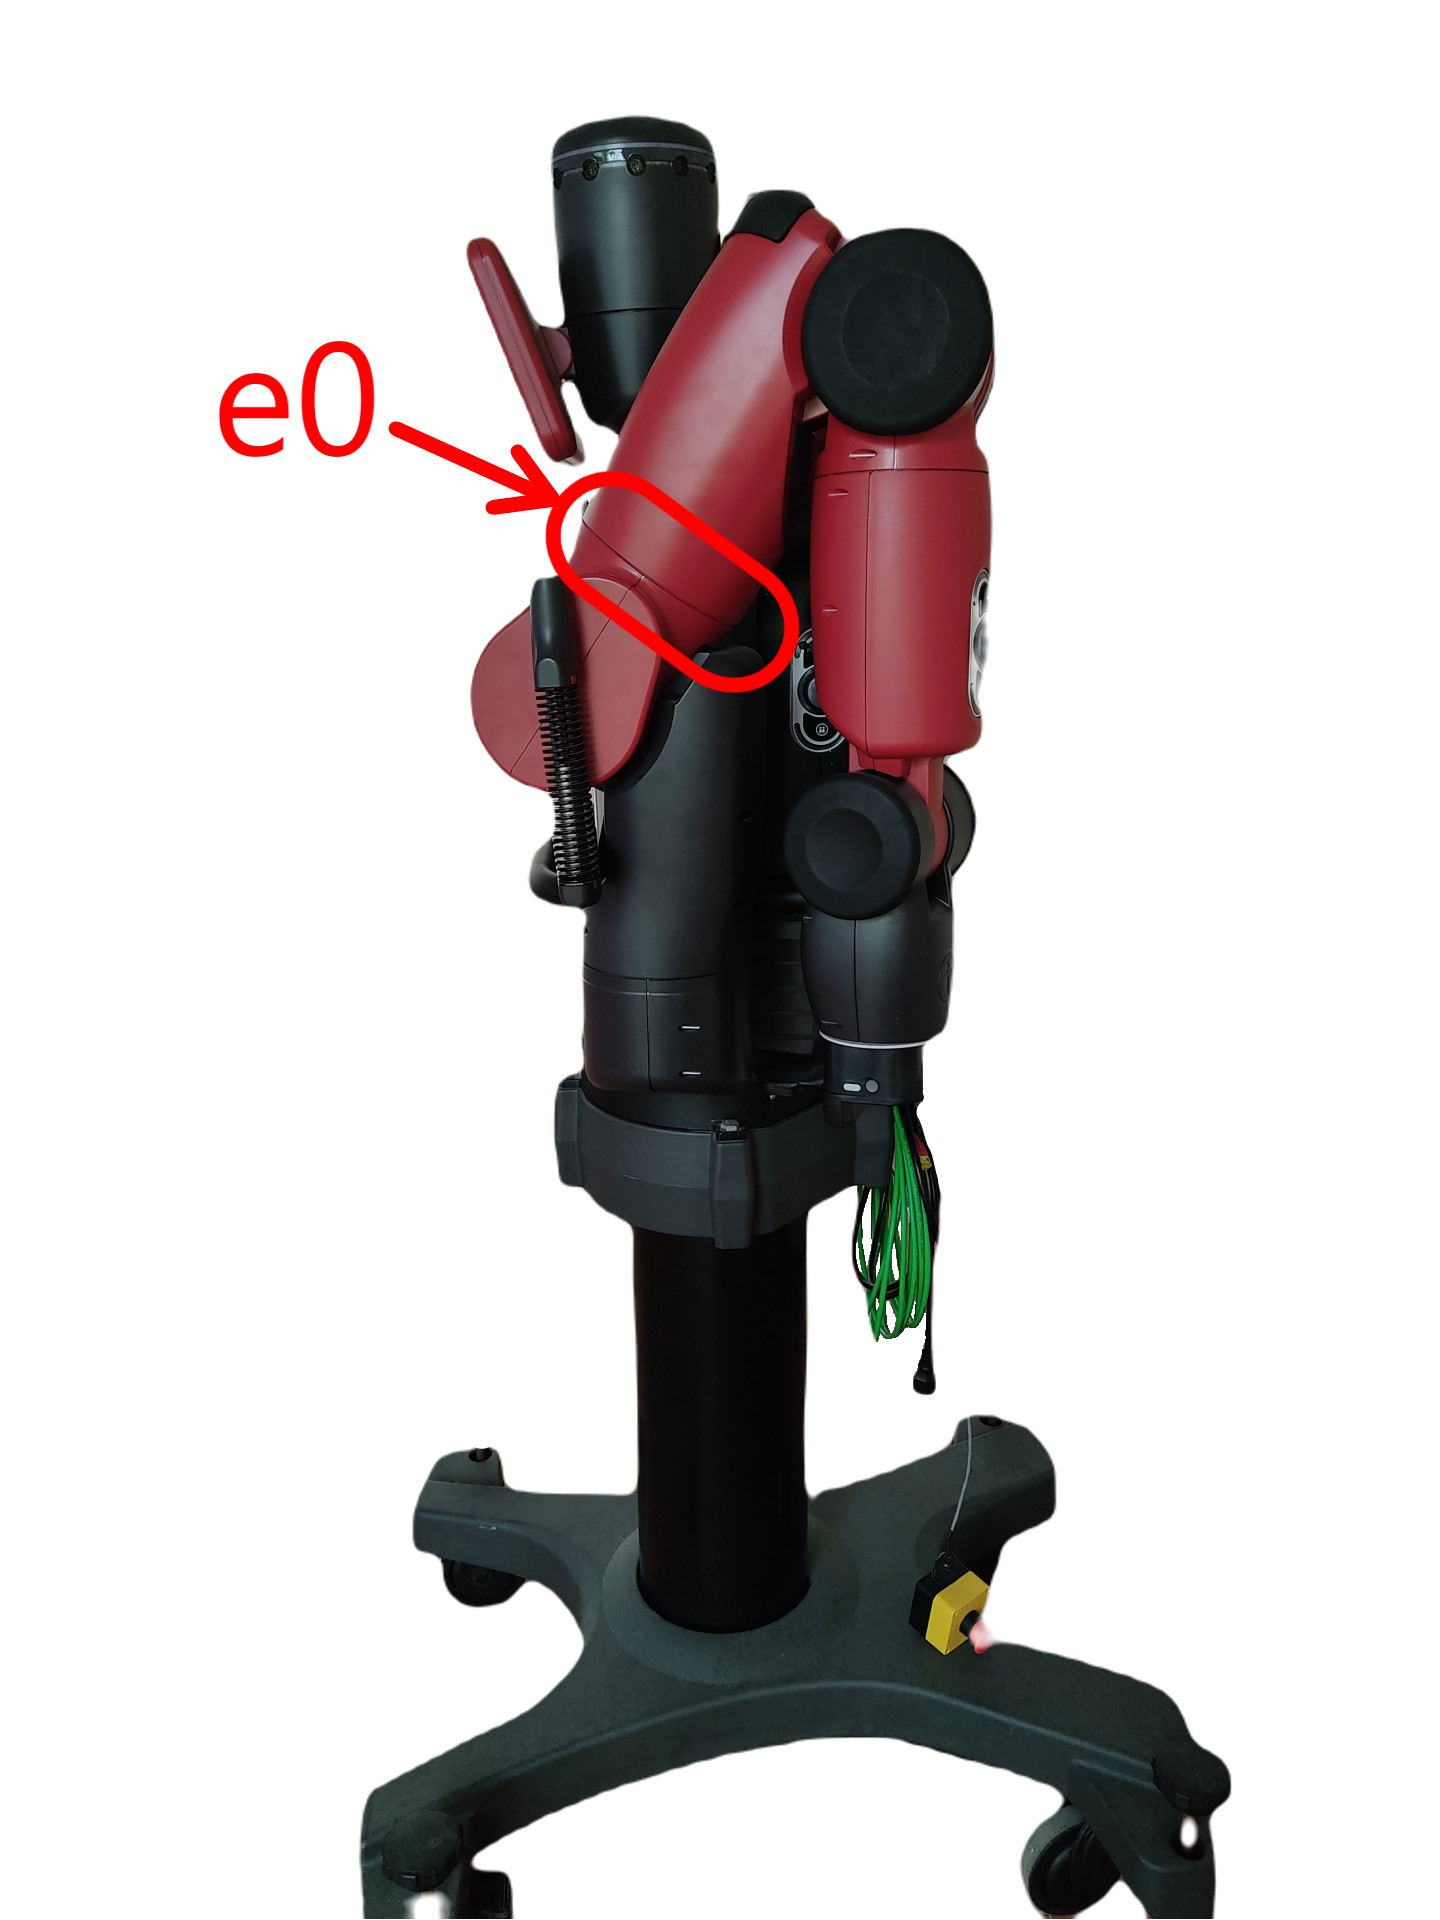
\includegraphics[width=0.6\linewidth]{assets/imgs/baxter_robot/baxter_left_tucked_no_background_showing_e0.jpg}
    \caption{Baxter e0 joint that will be fixed for the analytical IPK.} 
    \label{fig_baxter_fixed_e0_dof}
\end{figure}

Another important distance that will be discarded for this analytical calculation, is $L_5$, which is really small compared to the other limb distances. This assumption will make it simpler to obtain the analytical IPK Baxter solution.\\

After the $\theta_{3}$ and $L_5$ condition are said, the next part of the problem is to understand the inputs and outputs for getting the IPK.:\\

\textbf{Input Matrix:}

\begin{equ}[H]
\begin{equation} \label{eq:input_for_ipk}
    _{6}^{0}\textrm{T} = 
    \begin{bmatrix}
    r_{11} & r_{12} & r_{13} & _{}^{0}\textrm{x}_{6}\\ 
    r_{21} & r_{22} & r_{23} & _{}^{0}\textrm{y}_{6}\\ 
    r_{31} & r_{32} & r_{33} & _{}^{0}\textrm{z}_{6}\\ 
    0 & 0 & 0 & 1
    \end{bmatrix}
\end{equation}
\myequations{Input matrix for Inverse Pose Kinematic analytic solution.}
\caption{Input matrix for Inverse Pose Kinematic analytic solution.}
\end{equ}

\textbf{Output variables:}

\begin{equ}[H]
\begin{equation} \label{eq:output_for_ipk}
    [\theta_{1}, \theta_{2}, \theta_{4}, \theta_{5}, \theta_{6}, \theta_{7}]
\end{equation}
\myequations{Output variables for Inverse Pose Kinematic analytic solution.}
\caption{Output variables for Inverse Pose Kinematic analytic solution.}
\end{equ}

It is important to notice that the indices of the frames are assuming that $\theta_{3}$ is none, so they are shifted to the next one by one after the third DOF. This means that frames \say{4, 5, 6, 7} are now \say{3, 4, 5, 6}.\\

As well as that, keep in mind that the distance from the reference frames of joints \{2\} to \{4\}, is the euclidean distance from the center of each frame, that corresponds to: $\sqrt{L_{2}^2 + L_{3}^2}$.\\

The analytical solution can be proved by starting with equation shown in eq[\ref{eq:expression_to_obtain_analytical_ipk}], and applying linear algebra concepts for each one of the DOF.\\

\begin{equ}[H]
\begin{equation} \label{eq:expression_to_obtain_analytical_ipk}
    \begin{bmatrix}
    _{G_L}^{W_0}\textrm{T}
    \end{bmatrix}
    =
    \begin{bmatrix}
    _{B_L}^{W_0}\textrm{T}
    \end{bmatrix}
    \begin{bmatrix}
    _{0}^{B_L}\textrm{T}
    \end{bmatrix}
    \begin{bmatrix}
    _{6}^{0}\textrm{T}
    \end{bmatrix}
    \begin{bmatrix}
    _{G_L}^{6}\textrm{T}
    \end{bmatrix}
\end{equation}
\myequations{Expression to obtain the analytical IPK solution.}
\caption{Expression to obtain the analytical IPK solution.}
\end{equ}


The final angle values are:

\begin{equ}[H]
\begin{equation} \label{eq:angle_1_ipk}
    \theta_{1} = atan2(_{}^{0}\textrm{y}_{4}, _{}^{0}\textrm{x}_{4})
\end{equation}
\myequations{Joint angle 1 for the IPK solution}
\caption{Joint angle 1 for the IPK solution}
\end{equ}


\begin{equ}[H]
\begin{equation} \label{eq:angle_2_ipk}
\begin{split}
    x & = _{}^{0}\textrm{y}_{4} \\
    z & = _{}^{0}\textrm{z}_{4} \\
    E & = 2 \cdot L_{h} \cdot \left[L_{1} - \frac{x}{c_{1}}\right] \\
    F & = 2 \cdot L_{h} \cdot z \\
    G & = \frac{x^2}{c_{1}^2} + L_{1}^2 + L_{h}^2 - L_{4}^2 + z^2 - 2 \cdot \frac{L_{1} x}{c_{1}} \\
    t_{1,2} & = \frac{-F \pm \sqrt{E^2 + F^2 - G^2}}{G - E} \\
    \theta_{2_{1,2}} & = 2 atan(t_{1,2})
\end{split}
\end{equation}
\myequations{Joint angle 2 for the IPK solution}
\caption{Joint angle 2 for the IPK solution}
\end{equ}


\begin{equ}[H]
\begin{equation} \label{eq:angle_3_ipk}
    \theta_{4_{1,2}} = atan2(-z - L_{h}s_{2_{1,2}}, \frac{x}{c_{1}} - L_{1} - L_{h}c_{2_{1,2}}) - \theta_{2_{1,2}}
\end{equation}
\myequations{Joint angle 4 for the IPK solution}
\caption{Joint angle 4 for the IPK solution}
\end{equ}


\begin{equ}[H]
\begin{equation} \label{eq:rotation_matrix_3_6_for_ipk}
    \begin{bmatrix}
    _{6}^{3}\textrm{R}(\theta_{5}, \theta_{6}, \theta_{7})
    \end{bmatrix}
    =
    \begin{bmatrix}
    R_{11} & R_{12} & R_{13} \\ 
    R_{21} & R_{22} & R_{23} \\ 
    R_{31} & R_{32} & R_{33}
    \end{bmatrix}
\end{equation}
\myequations{Rotation matrix from reference frame 3 to reference frame 6 for the IPK procedure.}
\caption{Rotation matrix from reference frame 3 to reference frame 6 for the IPK procedure.}
\end{equ}


\begin{equ}[H]
\begin{equation} \label{eq:angle_5_ipk}
    \theta_{5} = atan2(R_{33}, R_{13})
\end{equation}
\myequations{Joint angle 5 for the IPK solution}
\caption{Joint angle 5 for the IPK solution}
\end{equ}

\begin{equ}[H]
\begin{equation} \label{eq:angle_6_ipk}
    \theta_{6} = atan2(\frac{R_{21}}{c_{7}}, -R_{23})
\end{equation}
\myequations{Joint angle 6 for the IPK solution}
\caption{Joint angle 6 for the IPK solution}
\end{equ}
\begin{equ}[H]
\begin{equation} \label{eq:angle_7_ipk}
    \theta_{7} = atan2(-R_{22}, R_{21})
\end{equation}
\myequations{Joint angle 7 for the IPK solution}
\caption{Joint angle 7 for the IPK solution}
\end{equ}


The Baxter IPK analytical solution will be a necessary algorithm to develop robotic solutions that map the Cartesian space to the joint space. This solution could be improved with a 7 DOF Inverse Pose Kinematics, but the cost of developing a solution that involves every join value, would represent a higher computational cost with lower response times for the robot.\\


To dive deeper into the software implementation of this algorithm, please feel free to explore our GitHub repository \say{baxter-bon-appetit} with the source code for the IPK:\\

\begin{itemize}
    \color{blue}
    \item \href{https://github.com/san99tiago/baxter-bon-appetit/blob/main/python/baxter_bon_appetit/src/baxter_essentials/baxter_ipk.py}{Baxter-Bon-Appetit Inverse Pose Kinematic Algorithm (Source Code)}
\end{itemize}


\subsection{Baxter Jacobian Analysis}
\label{subsection_baxter_jacobian_analysis}
The Jacobian is a matrix of partial derivatives of a vector function. It is extremely useful for finding transformation of coordinates systems.\\ 

In robotics, jacobian matrices are commonly used for  mapping joint velocities to Cartesian velocities \citep{cite_craig_robotics}. This mathematical tool enables a direct relationship between a fix world frame of a robot to its specific articulation frames.

It can be proved that the jacobians follow the mathematical expression:

\begin{equ}[H]
\begin{equation} \label{eq:transformation_matrices_for_dh_algorithm}
    \begin{bmatrix}
    _{}^{k}\textrm{J}
    \end{bmatrix}
    =
    \begin{bmatrix}
    \begin{bmatrix}
    _{w}^{k}\textrm{R}
    \end{bmatrix} & 0\\
    0 & \begin{bmatrix}
    _{w}^{k}\textrm{R}
    \end{bmatrix}
    \end{bmatrix}
    \begin{bmatrix}
    _{}^{w}\textrm{J}
    \end{bmatrix}
\end{equation}
\myequations{Jacobian transformation to another frame.}
\caption{Jacobian transformation to another frame.}
\end{equ}

Based on the article \say{Baxter Humanoid Robot Kinematics} \citep{cite_baxter_humanoid_robot_kinematics_ohio}, it is known the jacobian matrix from frame 4 to frame 0 ($_{}^{4}\textrm{J}$). This expression is really useful to calculate the jacobian matrix from frame 0 to the end-effector's frame.\\

The calculations and expressions to find Baxter's jacobian matrices can be found at the Baxter Bon Appetit GitHub repository:

\begin{itemize}
    \color{blue}
    \item \href{https://github.com/san99tiago/baxter-bon-appetit/blob/main/matlab/baxter_jacobian_calculation.m}{Baxter Jacobian calculation}
\end{itemize}

\begin{itemize}
    \color{blue}
    \item \href{https://github.com/san99tiago/baxter-bon-appetit/blob/main/python/baxter_bon_appetit/src/baxter_essentials/baxter_jacobian.py}{Baxter Jacobian implementation}
\end{itemize}

\section{Baxter Robot Work-Space}

A robot workspace is defined as the set of all reachable end-effector positions \citep{cite_robot_academy}. These multiple configurations could be theoretically infinite, but a general understanding of the workspace can be achieved with a rigorous mapping of the area.\\

For the further understanding of Baxter robot, this research developed a mapping algorithm that works in the following way:

\begin{center}
\includegraphics[width= 1.02\textwidth]{\string "assets/pdfs/baxter_robot/baxter_mapping_delaunay_block_diagram".pdf}
\bigbreak
\begin{minipage}{\linewidth} %Keep image/PDF in only 1 page
\captionof{figure}{Baxter mapping algorithm for calculating robot's workspace. Own development.}\label{fig_baxter_general_mapping_workspace_block_diagram}
\end{minipage} \end{center}

As it can be seen in fig[\ref{fig_baxter_general_mapping_workspace_block_diagram}], the mapping algorithm has the following steps:

\begin{enumerate}
    \item Move Baxter arms to the reachable positions and orientations to replicate multiple trajectories.
    \item From a JointState ROS Message, get the current Joint Angles measurements from the internal Baxter encoder sensors.
    \item Calculate current Cartesian coordinates from the Forward Pose Kinematics algorithms explained in the previous chapter.
    \item Repeat previous steps multiple times, appending the Cartesian coordinates to a database that holds multiple values for the Baxter mapping process.
    \item After the data is collected, apply these Cartesian values to the Delaunay Triangulation to obtain the desired workspace plot results.
\end{enumerate}

When the algorithm was implemented for the mapping, the first results were the \say{General Mapping Workspace Trajectories}, that would cover most of Baxter workspace. These trajectories were taken with the explained algorithm for 30 minutes in each of Baxter's arms. It is important to notice, that to avoid robot damage, the trajectories were implemented by moving Baxter arms manually by touching the cuff sensor and driving the arms as much as possible.\\

\begin{figure}[H]
    \centering
    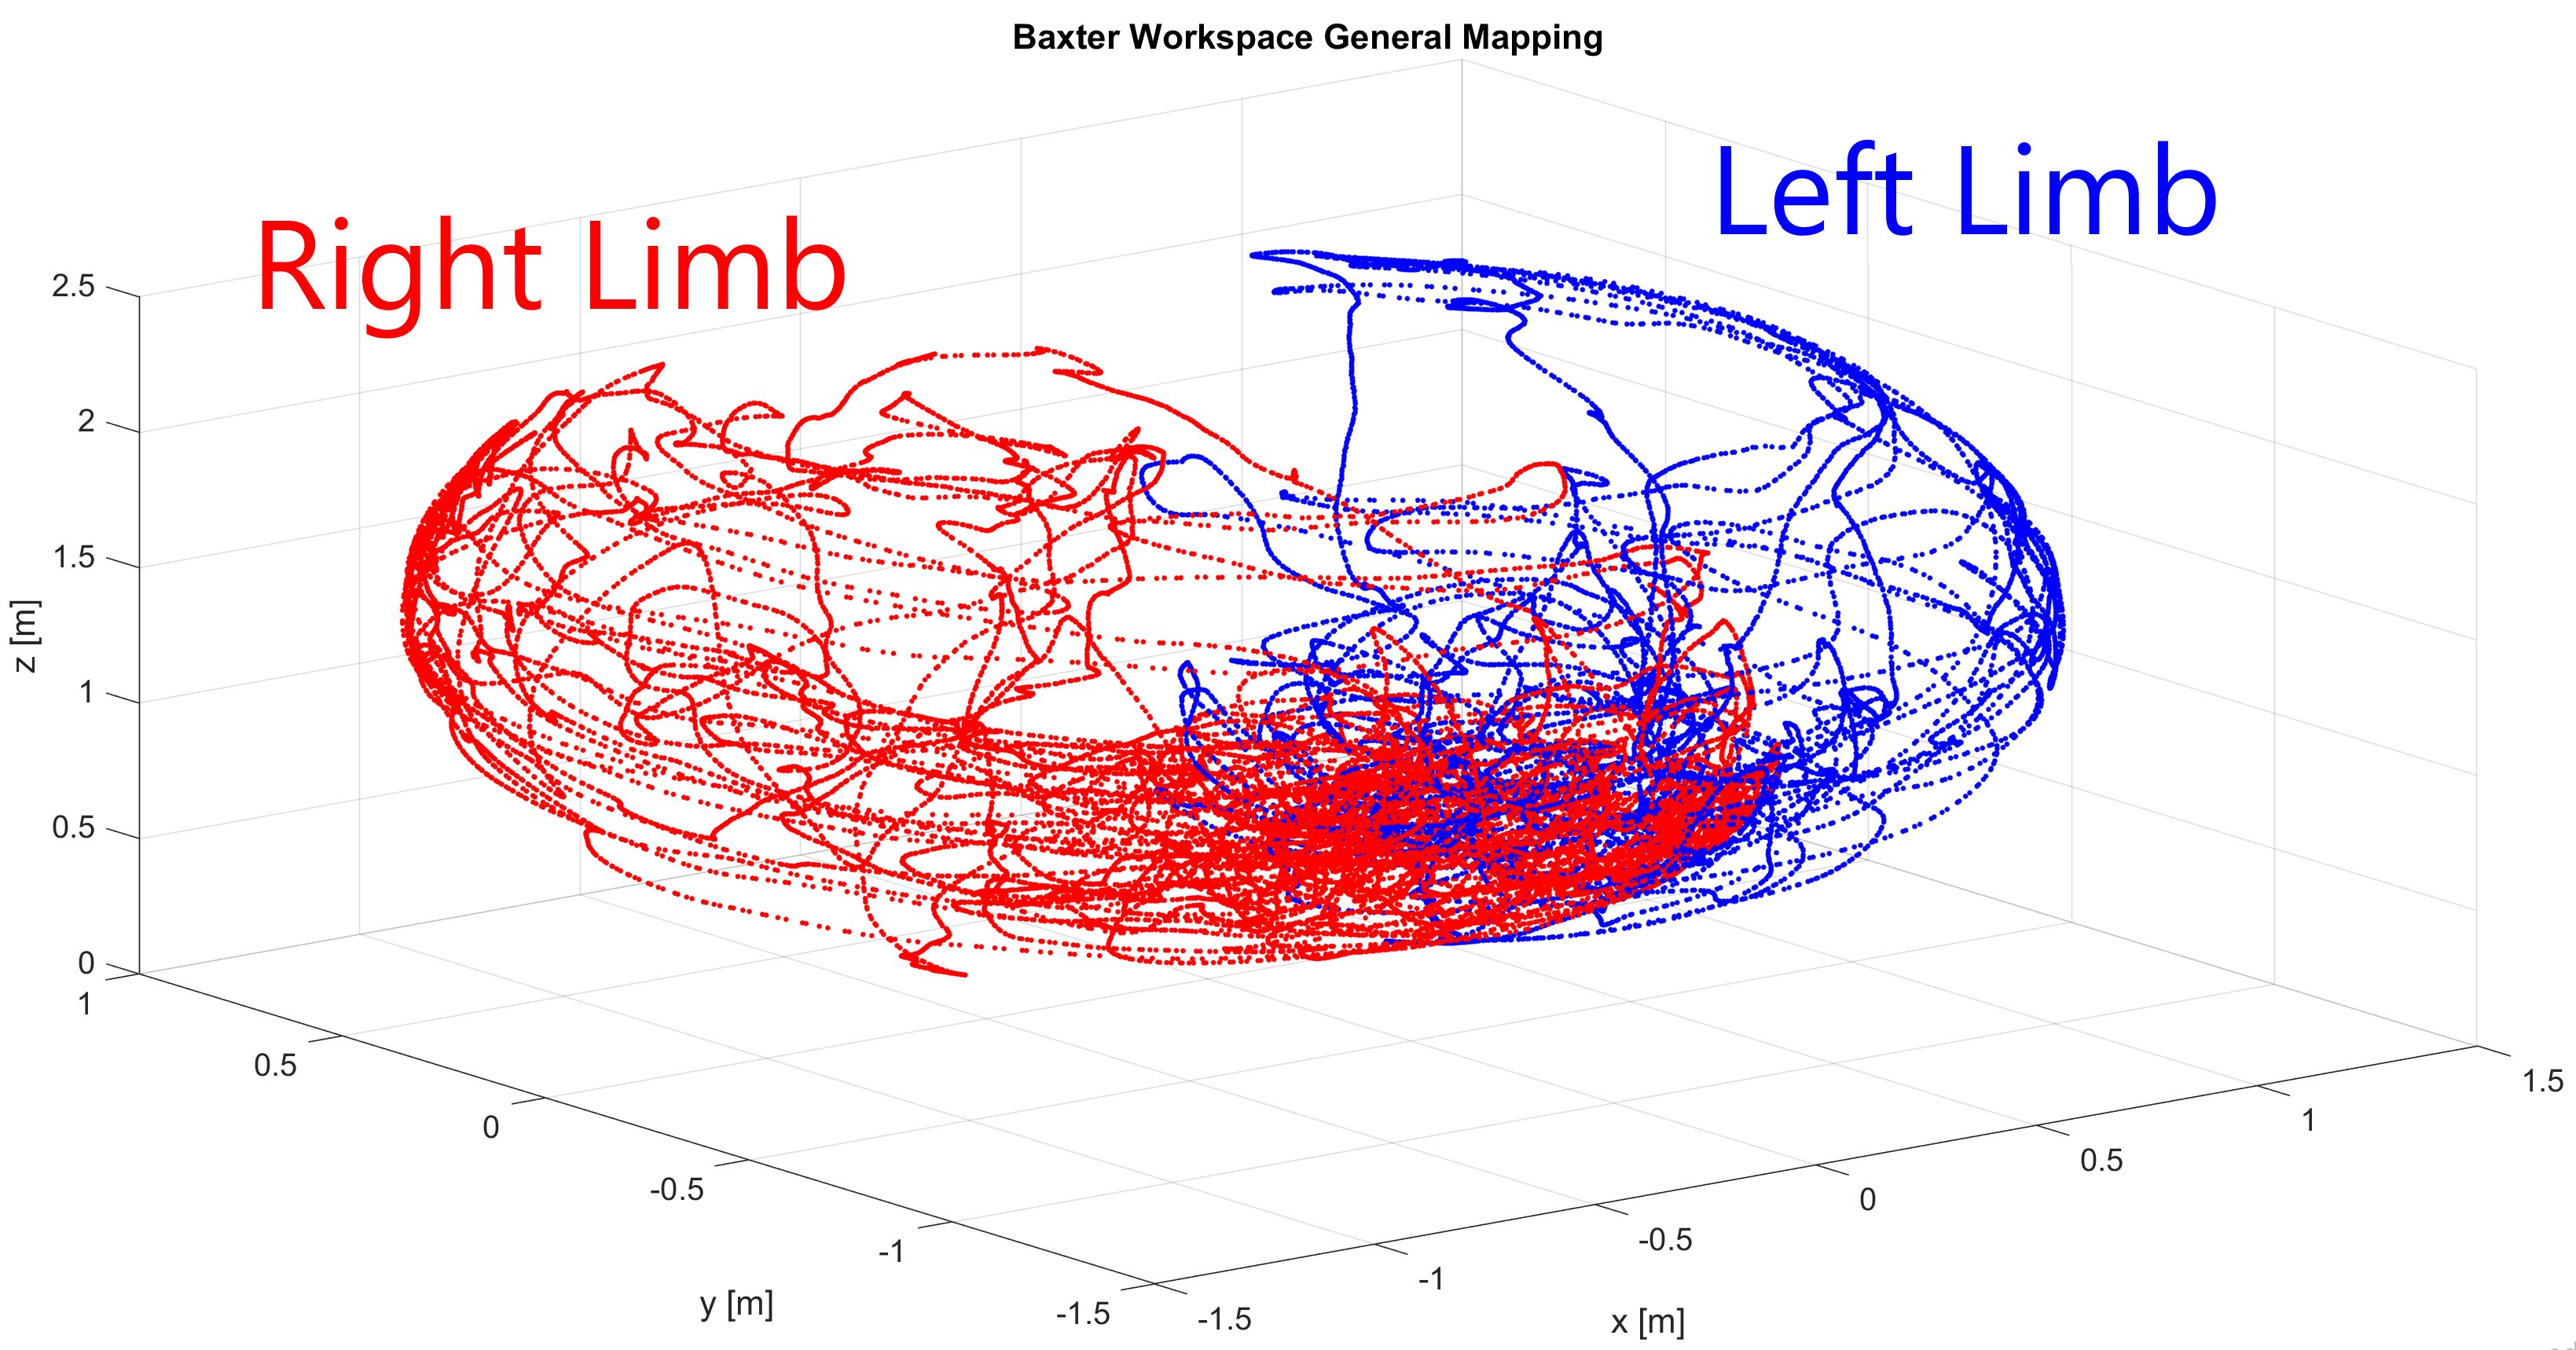
\includegraphics[width=0.92\linewidth]{assets/imgs/baxter_robot/baxter_workspace_general_mapping.png}
    \caption{Baxter robot general mapping for the workspace. Own development.} 
    \label{fig_baxter_general_workspace}
\end{figure}

After the database of the trajectories for the Cartesian values was filled, the Delaunay Triangulation was applied to the overall results. The objective of this process, was to obtain the maximum reachable spherical surface for Baxter robot workspace. The result is extremely valuable, because it gives us some important information, such as:

\begin{itemize}
    \item Baxter robot's workspace shape and symmetry.
    \item Baxter robot's limits for X, Y, and Z dimensions.
    \item Overview of good and bad manoeuvrability positions for both of Baxter's arms.
    \item A good understanding of the mathematics to relate joint-states with Cartesian-coordinates.
\end{itemize}


\begin{figure}[H]
    \centering
    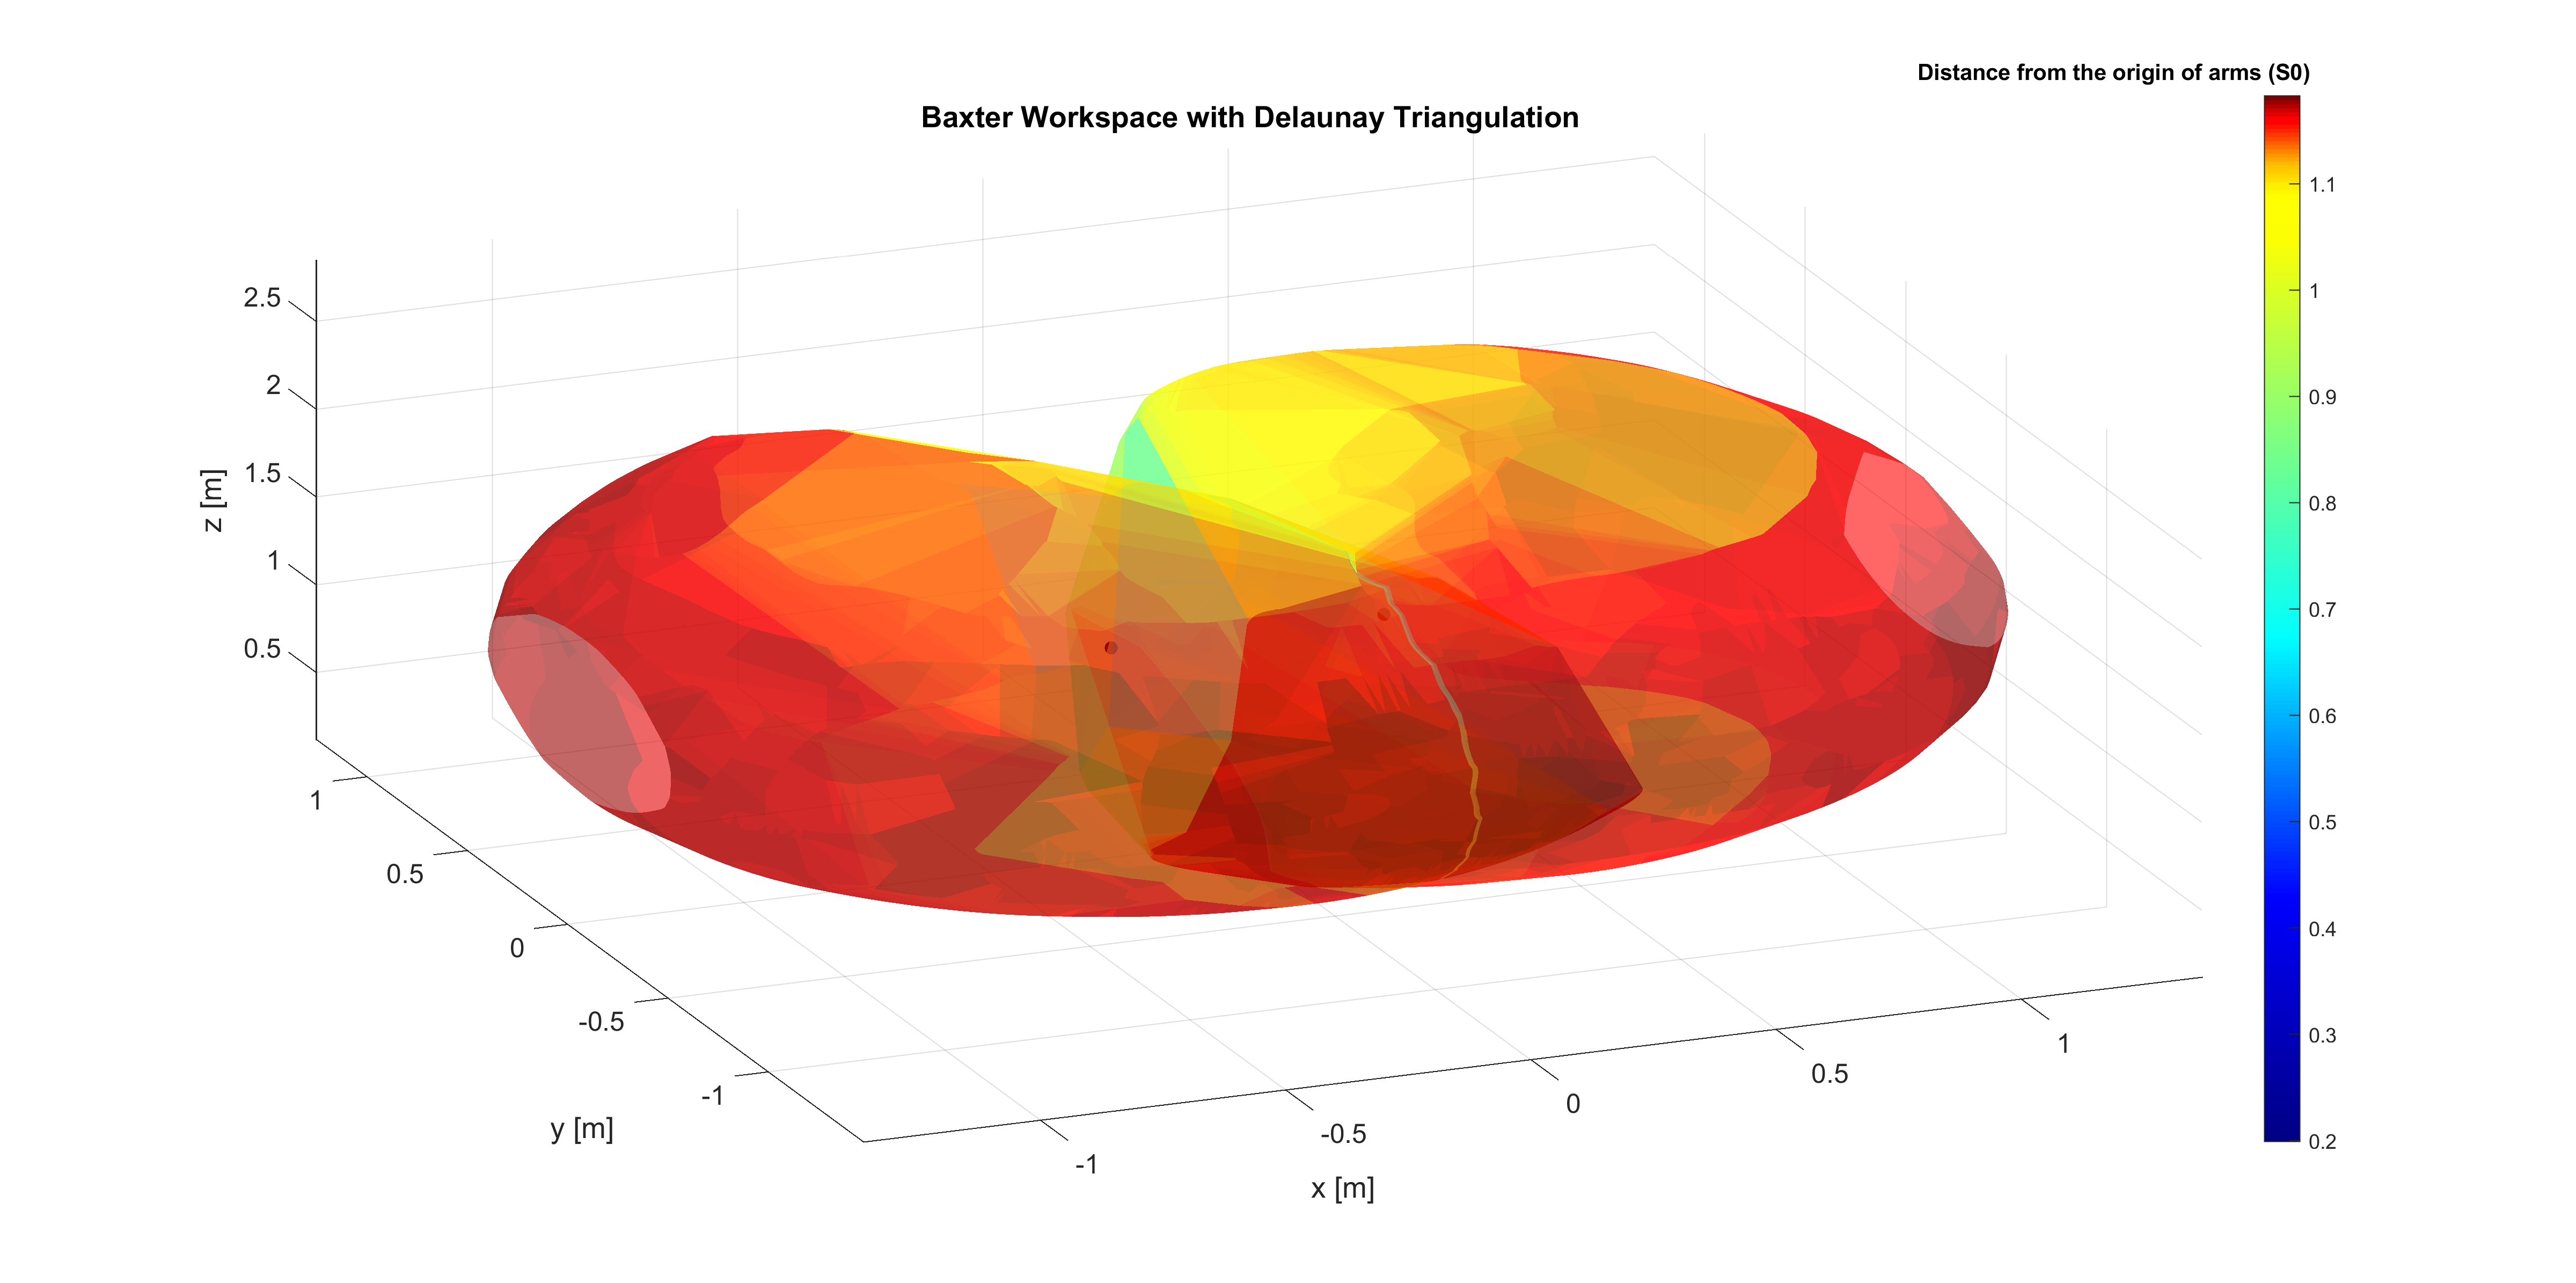
\includegraphics[width=1.0\linewidth]{assets/imgs/baxter_robot/baxter_workspace_delaunay_triangulation.png}
    \caption{Baxter workspace after Delaunay Triangulation. Own development.} 
    \label{fig_workspace_after_delaunay_triangulation}
\end{figure}


The algorithms to map Baxter workspace can be analyzed at our GitHub repository \say{baxter-bon-appetit} with the source code for both processes explained in fig[\ref{fig_baxter_general_mapping_workspace_block_diagram}]:\\

\begin{itemize}
    \color{blue}
    \item \href{https://github.com/san99tiago/baxter-bon-appetit/blob/main/matlab/Baxter_Workspace.m}{Baxter-Bon-Appetit MATLAB Delaunay Triangulation Algorithm (Source Code)}
    \color{blue}
    \item \href{https://github.com/san99tiago/baxter-bon-appetit/blob/main/python/baxter_bon_appetit/scripts/map_workspace.py}{Baxter-Bon-Appetit Map Workspace Algorithm (Source Code)}
\end{itemize}


\section{Baxter Robot Tool}

A robot's tool corresponds to a functional extension of the robot's basic capabilities. This final component not only implies a change in the mathematical equations governing the robot's dynamics, but also allows extending the practical behavior of the features that the robot can perform in its classical programming.\\

For this application (Baxter-Bon-Appetit), the most important capability to be implemented with Baxter robot, is to be able to carry out food for an user. This circumstances, imply that the tool designed for Baxter robot must follow up a series of requirements, such as:

\begin{itemize}
    \item The tool must be able to be placed firmly on Baxter hand.
    \item The tool must carry out (hold) food.
    \item The tool must be able to carry different cutlery utensils, so that they can be changed easily depending on the patient and type of food. 
\end{itemize}

After taking into consideration these requirements, it was chosen that a 3D printed design would satisfy all the requirements and be cost-efficient for the economic budget of this research project. The 3D printed approach was a viable way to develop an accurate mechanical tool, that would match the necessary tolerances of Baxter's arms.\\

First of all, the software in which the design was made, was Autodesk Fusion 360, a cloud-based 3D modeling, CAD, CAM, CAE, and PCB software platform for product design and manufacturing \citep{cite_autodesk_fusion}. This allowed us to work simultaneously on the design and develop a practical re-usable tool system.\\

The design of tool had to match the following Baxter hand attaching system, so that it could be placed correctly and guarantee a stable connection to Baxter arm:

\begin{figure}[H]
    \centering
    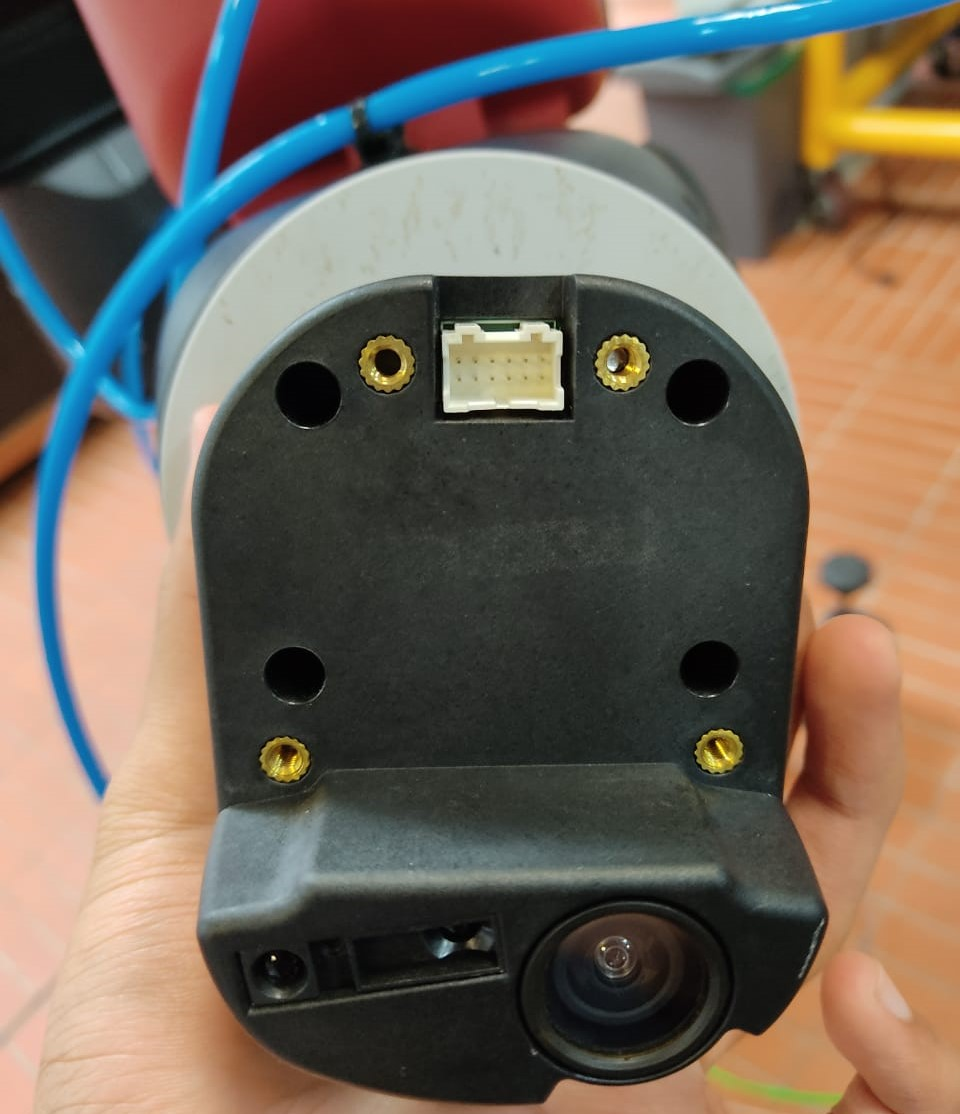
\includegraphics[width=0.6\linewidth]{assets/imgs/baxter_robot/baxter_hand_before_tool.jpeg}
    \caption{Baxter hand for attaching the tool. Taken at EIA University Laboratory.} 
    \label{fig_baxter_hand_for_attaching_the_tool}
\end{figure}

Based on the hand, it was developed a design that matched the default Baxter mechanism for adding external tools designed by the user. This solution was developed as a stereo-lithography CAD design (also known as STL), which is an universal format that can be understood by most CAD-CAM software and 3D printers.\\

The overall mechanical solution achieved for Baxter-Bon-Appetit research project with Fusion 360 software can be seen at figs[\ref{fig_baxter_tool_fusion_front_view}, \ref{fig_baxter_tool_fusion_multiple_views}]:

\begin{figure}[H]
    \centering
    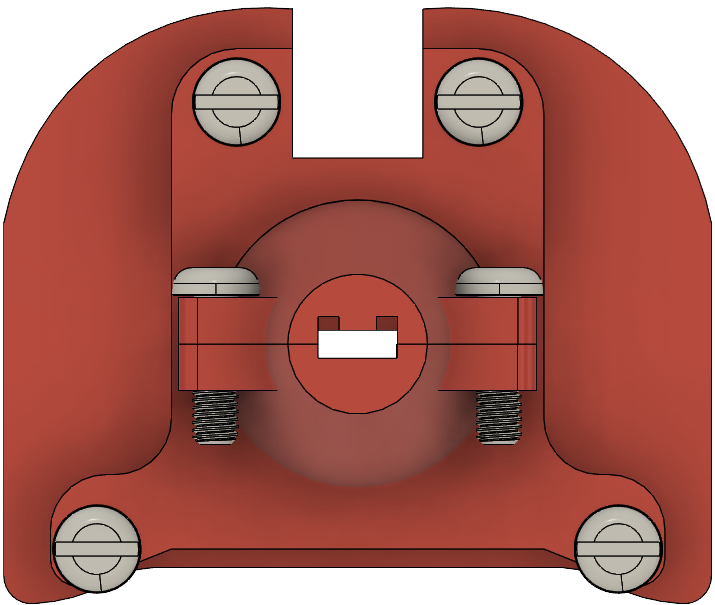
\includegraphics[width=0.6\linewidth]{assets/imgs/baxter_robot/baxter_spoon_fusion_front_view.png}
    \caption{Baxter tool front view in Fusion 360 software. Own development.} 
    \label{fig_baxter_tool_fusion_front_view}
\end{figure}


One important advantage that is full-filled with the developed design, is that there can be multiple cutlery coupled in the tool, so that the user can change the necessary cutlery, based on the food that he or she wants and also be able to change them based on the user (for more than one different patient).\\


\begin{figure}[H]
	\centering
	\begin{subfigure}{.5\textwidth}
		\centering
		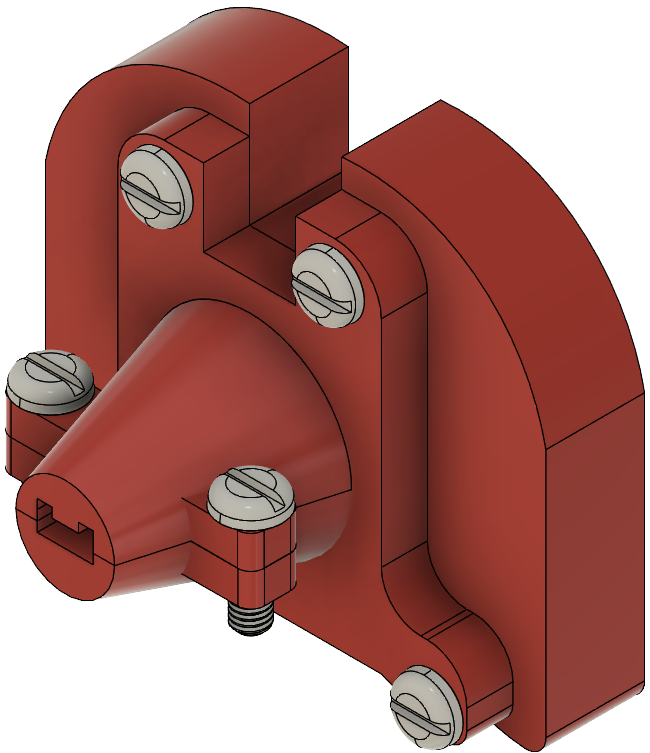
\includegraphics[width=0.65\linewidth]{assets/imgs/baxter_robot/baxter_spoon_fusion_side_view_closed.png}
		\caption{Baxter tool general view closed. Own development.}
		\label{fig_general_view_baxter_tool_closed}
	\end{subfigure}~
	\begin{subfigure}{.5\textwidth}
		\centering
		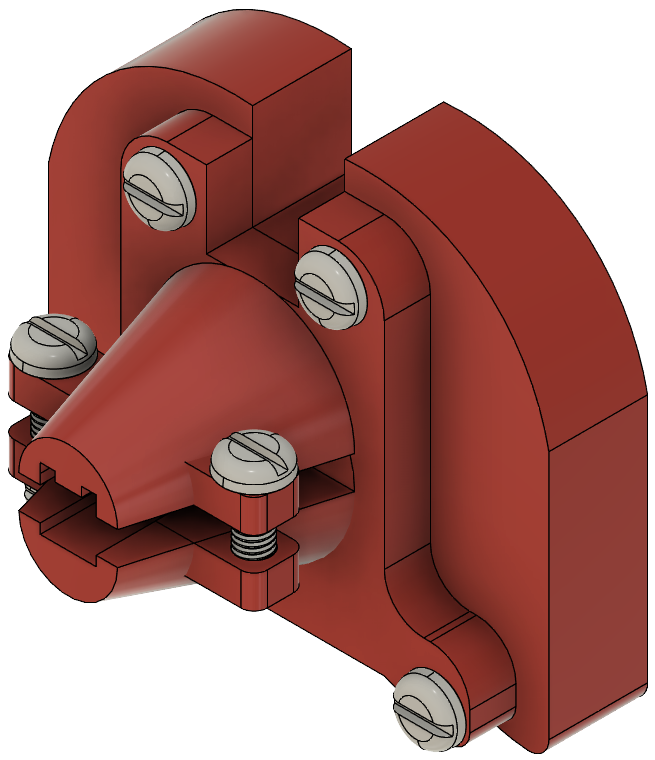
\includegraphics[width=0.65\linewidth]{assets/imgs/baxter_robot/baxter_spoon_fusion_side_view_opened.png}
		\caption{Baxter tool general view opened. Own development.}
		\label{fig_general_view_baxter_tool_opened}
	\end{subfigure}%
	\caption{Baxter tool viewed opened and closed for attaching the cutlery. Own development.}
	\label{fig_baxter_tool_fusion_multiple_views}
\end{figure}


After the general measurements were implemented and verified at the CAD STL design, the next step was to print it into a real tool by a 3D printer. This process was achieved successfully with the \say{Ender-3 V2 3D Printer}, a low-price system, suitable for business start-ups and research projects \citep{cite_3d_printer_for_tool}.\\

This 3D printer was able to create the tool in 4 hours and 30 minutes. The reason of this time, is because the tool was created with a high-density speed constant, so that it would be more resistant to fatigue and mechanical stresses.\\

\begin{figure}[H]
	\centering
	\begin{subfigure}{.5\textwidth}
		\centering
		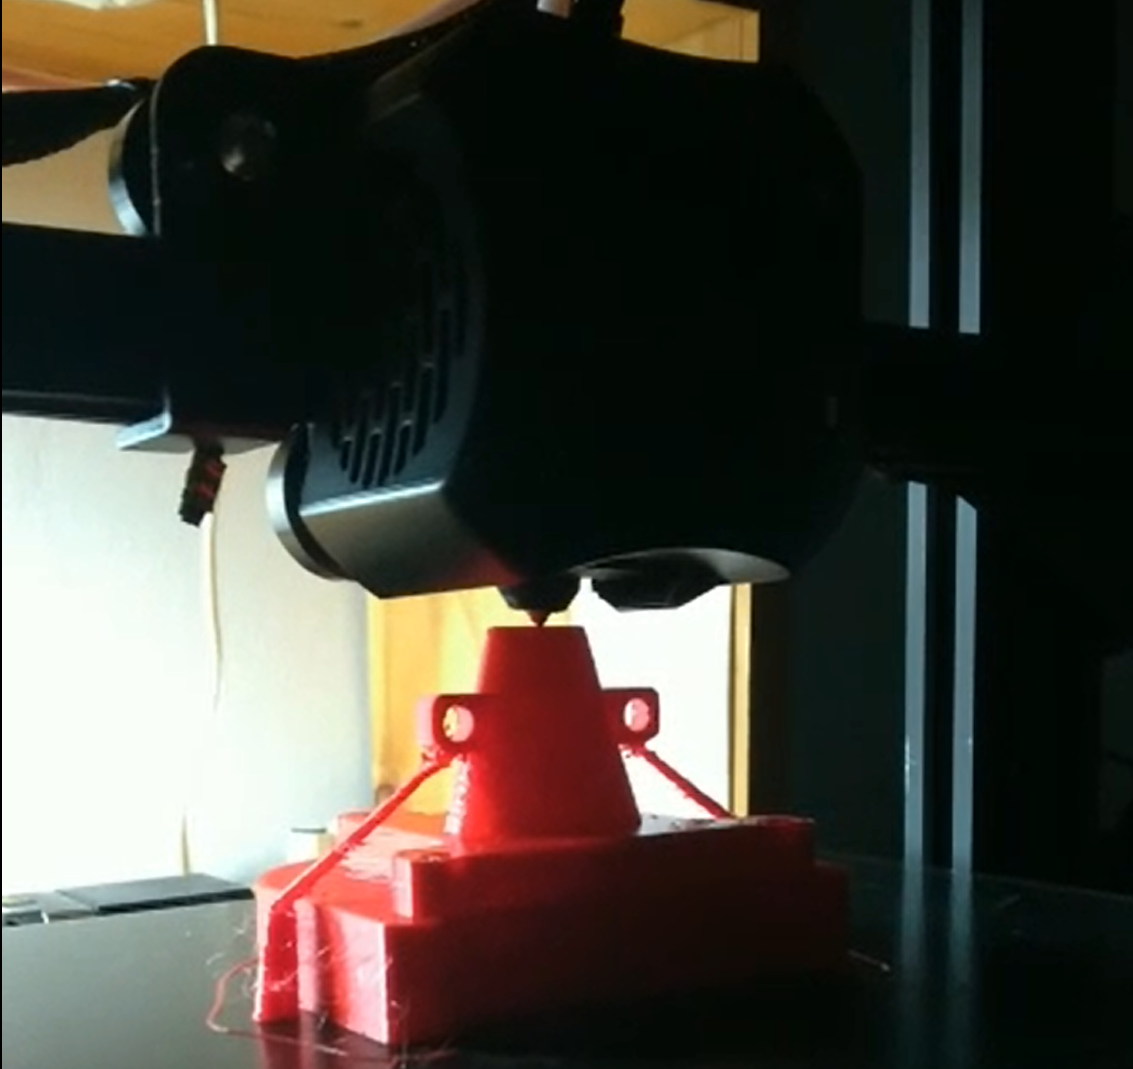
\includegraphics[width=0.87\linewidth]{assets/imgs/baxter_robot/baxter_spoon_process_printing.png}
		\caption{Printing process of Baxter tool in action.}
		\label{fig_3d_prniter_in_action_1}
	\end{subfigure}~
	\begin{subfigure}{.5\textwidth}
		\centering
		\includegraphics[width=0.8\linewidth]{assets/imgs/baxter_robot/baxter_spoon_process_end.jpeg}
		\caption{Printing process of Baxter tool finished.}
		\label{fig_3d_prniter_in_action_2}
	\end{subfigure}%
	\caption{Baxter tool 3D printing process.}
	\label{fig_baxter_tool_printing_process}
\end{figure}


When the design was completely printed, the next part of the methodology was to verify that it could fit correctly (and properly) into Baxter's hand. This was verified and was achieved successfully at EIA University Laboratory.\\

The following images show the final result of Baxter's tool to correctly be able to give food to the users in a correct and natural way:

\begin{figure}[H]
    \centering
    \includegraphics[width=0.6\linewidth]{assets/imgs/baxter_robot/baxter_tool_real_life_implementation.jpg}
    \caption{Baxter tool general view implemented on real life. Taken at EIA University Laboratory.} 
    \label{fig_baxter_tool_real_life_general_view}
\end{figure}

\begin{figure}[H]
    \centering
    \includegraphics[width=0.8\linewidth]{assets/imgs/baxter_robot/baxter_tool_real_life_implementation_side_view.jpg}
    \caption{Baxter tool side view implemented on real life. Taken at EIA University Laboratory.} 
    \label{fig_baxter_tool_real_life_side_view}
\end{figure}

The results of Baxter tool for giving food correctly, will be considered as an important condition to take into account in the mathematical calibrations of the FPK algorithm (as an additional offset of the final Baxter hand transformation).\\

\section{Baxter Physical Configuration}

For Baxter-Bon-Appetit project, the physical workspace configuration for the robot/patient space is a differential factor to fulfill the development of an active feeding system. This configuration is a deterministic decision that will guide the design of the solution and will modify the evolution of the project based on how it is chosen.\\

To determine the physical configuration, there are some key values to take into consideration:

\begin{enumerate}
    \item The patient must be seated facing directly to one of Baxter's cameras.
    \item The patient must be located in a place where Baxter maneuverability is high.
    \item The position of the camera and the patient should be always the same (or really similar).
\end{enumerate}

Based on these user requirements, the chosen configuration for Baxter and the patient is the one shown in figures fig[\ref{fig_baxter_configuration_1},\ref{fig_baxter_configuration_2}]:

\begin{center}
\includegraphics[width= 1.02\textwidth]{\string "assets/pdfs/baxter_robot/baxter_setup_physical_configuration".pdf}
\bigbreak
\begin{minipage}{\linewidth} %Keep image/PDF in only 1 page
\captionof{figure}{Baxter physical configuration explained. Own development.}\label{fig_baxter_configuration_1}
\end{minipage} \end{center}

\begin{figure}[H]
	\centering
	\begin{subfigure}{.5\textwidth}
		\centering
		\includegraphics[width=1.0\linewidth]{assets/imgs/baxter_robot/computer_vision_side_view_elkin_eating.png}
		\caption{Physical configuration for Baxter and the user (side view). Taken at EIA University Laboratory.}
		\label{fig_baxter_configuration_2a}
	\end{subfigure}~
	\begin{subfigure}{.5\textwidth}
		\centering
		\includegraphics[width=1.0\linewidth]{assets/imgs/baxter_robot/computer_vision_front_view_elkin_eating.png}
		\caption{Physical configuration for Baxter and the user (front view). Taken at EIA University Laboratory.}
		\label{fig_baxter_configuration_2b}
	\end{subfigure}%
	\caption{Physical configuration for Baxter and the user. Taken at EIA University Laboratory.}
	\label{fig_baxter_configuration_2}
\end{figure}


As it can be seen in the shown figures, the configuration was chosen because Baxter's right arm can reach the user's mouth directly in order to do the feeding action. This will enable Baxter cobot to have a great functionality of helping the patient to eat his meal in a dynamic and active way.\\

Another remarkable condition of the exposed arrangement, is that the camera that is going to be used is directly embedded on Baxter's left arm, implying that it can be tweaked in position and orientation (something that would not be achievable with the camera on Baxter's head). As well as this extra translation and rotation approach, one advantage of using a camera that is directly designed into Baxter's arm, is that, with the encoder measurements, it will always be possible to find the current position of the camera (even after external modifications). This measurements will be explained in future chapters.\\

One extra interesting benefit of implementing this physical layout, is that the patient will always be facing directly to the camera, and even after having its meal given to his mouth, his face will be mostly visible to the camera, resulting in a great clear-vision approach for constantly detecting the user's face.\\

The research will use the exposed configuration for the control, computer vision and integration algorithms.\\

% ---------------------------------------------------------
\chapter{Computer Vision}

Most robotic systems that are aware of their environment, use sensors of various types to ensure proper data acquisition to provide valuable information for the dynamic variables of interest for the system.\\

For the case in which cameras are used as primary sensors, it is extremely important to understand that the acquired signal can not go directly to a control scheme, but must be processed and debugged through computational algorithms that transform the multiple RGB matrices obtained by these cameras, in more accurate variables according to the control scheme.\\

The computer vision algorithms that will be implemented on Baxter robot, will start directly from the embedded robot's cameras, as it was described in the design exposed at fig[\ref{fig_general_morphological_matrix}]. This decision

\section{Baxter Camera Configuration and Setup}

To implement a computer vision algorithm, it is relevant to have a deep understanding on the camera specifications. The most relevant characteristics for Baxter cameras are exposed in table tab[\ref{tab:camera_specifications}] and it is important to guarantee that the camera's resolution is fixed in a constant value (so that the trained networks work properly).\\

The chosen value for the camera resolution is \say{640x400 pixels}. This value is obtained from the best practices specifications given in Baxter camera SDK documentation \citep{cite_baxter_hardware_specifications}.\\

The software and mathematical implementations for this chapter, will be calculated based on the chosen resolution of Baxter's left hand camera, so that the algorithms work in a proper way.\\

\section{Baxter Camera Manipulation}

To understand how Baxter's cameras work, we highly recommend to dive deeper into the official SDK documentation, so that every detail can be considered \citep{cite_baxter_cameras_wiki}.\\

Baxter cameras are relevant sensors designed to gather direct information from Baxter's environment as fast as possible. These devices are assembled and integrated with Baxter functionalities through ROS. To control the cameras and the information acquired, we must understand some key features:

\begin{itemize}
    \item Cameras are controlled with an Application Programming Interface (API) that makes it possible to interact with their software configurations.
    \item Camera information is understood as ROS messages and topics that are constantly being updated and published based on the requirements.
    \item To read Baxter's cameras photos/videos, they must be transformed into a standard image matrix-wise format.
    \item Only two out of the three Baxter's cameras can operated at the same time.
\end{itemize}

For the discovery of Baxter's cameras and their functionalities, 
the robot was controlled and operated through the official camera control algorithms given by Rethink Robotics:

\begin{itemize}
    \color{blue}
    \item \href{https://github.com/RethinkRobotics/baxter_tools/blob/master/scripts/camera_control.py}{RethinkRobotics/baxter\_tools: camera control (Source Code)}
\end{itemize}

After understanding the underlying low-level configurations, the computer vision algorithms designed for this research, were developed using the internal messages of Baxter robot regarding its cameras and the necessary subscribers to their information. A deeper analysis of these implementations, will be discussed in the source code and in ROS integration section.\\


\section{Face Detection Algorithms}

For Baxter-Bon-Appetit project, the face detection algorithms are considered to be one on the first key components of the whole control structure. This is due because they convert the original images obtained from Baxter's cameras (complex matrices that do not give straight valuable information), into strategical information that is understood as a reference feature for mapping the user's face.\\

The two algorithms that are going to be developed for this research, are variants of:

\begin{enumerate}
    \item Vioja-Jones Classifier with Haar Cascade Feature Selection.
    \item Face Recognition API based on deep learning using dblib.
\end{enumerate}

Both face detection algorithms are going to be built on top of the ones mentioned, as a particular extension of their functionalities.\\

\subsection{Viola-Jones Classifier}
\label{sec:viola_jones_classifier}

The Viola-Jones classifier was developed by Paul Viola , Michael Jones, and it was one of the pioneer programs to correctly solve the face detection problem in a fast and accurate way \citep{cite_viola_jones_face_detection_algorithm}. The problem that it solved was to be able to detect any face in a given input image.\\

This algorithm expects the face to be positioned directly to the camera so that it is arranged as a frontal upright face. As well as this, it important that the face is not tilted to either one of the sides, avoiding inclinations.\\

\begin{center}
\includegraphics[width= 1.02\textwidth]{\string "assets/pdfs/computer_vision/computer_vision_haar_cascade_block_diagram".pdf}
\bigbreak
\begin{minipage}{\linewidth} %Keep image/PDF in only 1 page
\captionof{figure}{Face detection block diagram implementing Viola-Jones Haar Cascade Classifier and AdaBost. Own development.}\label{fig_computer_vision_block_diagram_haar_cascade}
\end{minipage} \end{center}

The algorithm that was developed on top of Viola-Jones classifier, has multiple extra inputs, such as frequency, video acquisition, scale factors, minimum neighbors, minimum size and other internal parameters.\\

The described face detection algorithm was developed with Python programming language with the libraries of OpenCV and numpy. The source code of Baxter Bon Appetit project for face detection with Viola-Jones approach, can be found at \say{baxter-bon-appetit} GitHub repository:


\begin{itemize}
    \color{blue}
    \item \href{https://github.com/san99tiago/baxter-bon-appetit/tree/main/python/computer_vision/face_detect_haar_cascade}{Baxter-Bon-Appetit Face Detecion Algorithm based on Viola-Jones Framework (Source Code)}
\end{itemize}


Each one of the steps of the block diagram is going to be explained with a high level of abstraction:

\subsubsection{Get frames of video based on desired frequency}

This process is the one that manages how the input to the OpenCV Haar Cascade Classifier is going to be analyzed. This implies, that the sample time and video conditions are configured as general inputs to the algorithm.\\

To do this step, a continuous loop is processing the video input in a Python Thread, and it has specific wait times to only process the video input at a desired time. This processing converts the video frames into specific images with a given window size.\\

\subsubsection{Haar feature selection}

Feature selection is a mandatory step in object detection algorithms. For Viola-Jones detection framework, the Haar feature selection has to process and analyze more than 180.000 features (in a 24x24 average image), and has the main goal of getting the useful features and reducing the overall processing time.\\

The four basic Haar features implemented in Viola-Jones algorithm are:

\begin{figure}[H]
    \centering
    \includegraphics[width=0.6\linewidth]{assets/imgs/computer_vision/viola_jones_haar_features.png}
    \caption{Example of Haar features used for Viola-Jones algorithm. Taken from \citep{cite_haar_features_example_viola_jones}.} 
    \label{fig_viola_jones_features_example}
\end{figure}

These features will play a special role in the determination of what is a face or not. These features must be calculated and analyzed in a short amount of time and the selection of the relevant ones is usually implemented with criteria such as:

\begin{enumerate}
    \item Horizontal white-black feature.
    \item Vertical white-black feature.
    \item Vertical white-black-white feature.
    \item Diagonal white-black feature.
\end{enumerate}

\subsubsection{Integral Image}

The integral image approach, also known as summed-area-table is a data structure and algorithm that is commonly used in computer vision and computer graphics \citep{cite_matlab_integral_image}. This process calculates the sum of the values of a matrix in a subsection of the grid. This implies that the original matrix is then processed into a new integral matrix that has relevant values of the inner elements sums.\\

The advantage of generating integral images, is that they reduce significantly the amount of operations involved in computer vision algorithms, and therefore, they improve the performance of the algorithm undoubtedly.\\

The process of generating an integral image is based on the following equation:

\begin{equ}[H]
\begin{equation} \label{eq:integral_image_equation}
    \begin{split}
        ii(x, y) = \sum_{x'<=x,y'<=y}^{} i(x', y') \\
        ii(x, y) = \text{Integral Image} \\
        i(x, y) = \text{Original Image} \\
    \end{split}
\end{equation}
\myequations{Equations for integral image calculation}
\caption{Equations for integral image calculation}
\end{equ}

This algorithm sums up the corresponding image pixels, and generates the final integral image that will be implemented in the following steps.\\


\begin{figure}[H]
	\centering
	\begin{subfigure}{.5\textwidth}
		\centering
		\includegraphics[width=0.7\linewidth]{assets/imgs/computer_vision/integral_image_calculation_part01.png}
		\caption{Original image. Taken from \citep{cite_integral_image_photo_wikipedia}}
		\label{fig_integral_image_part01}
	\end{subfigure}~
	\begin{subfigure}{.5\textwidth}
		\centering
		\includegraphics[width=0.55\linewidth]{assets/imgs/computer_vision/integral_image_calculation_part02.png}
		\caption{Result of integral image calculation. Taken from \citep{cite_integral_image_photo_wikipedia}}
		\label{fig_integral_image_part02}
	\end{subfigure}%
	\caption{Example of a process of integral image calculation.}
	\label{fig_integral_image_complete}
\end{figure}



\subsubsection{AdaBoost Training}

The AdaBoost training, also called Adaptive Boosting, is an ensemble method in Machine Learning algorithms. In order to understand the adaBoost method, it is necessary to know how the boosting algorithm actually works, this technique makes 'n' number of decisions trees during the data training time, as the first decision tree/model is made, the incorrectly classified record in the first model is given priority. Only these records are sent as input for the second model. The process goes on until we specify a number of base learners we want to create \citep{cite_adaboost_explained}.

\begin{figure}[H]
    \centering
    \includegraphics[width=0.8\linewidth]{assets/imgs/computer_vision/decition_trees.png}
    \caption{Example of the decision trees created in the training period by boosting technique. Taken from \citep{cite_adaboost_explained}.} 
    \label{fig_adaboost_explained}
\end{figure}

In AdaBoost algorithm, the main objective is to improve the performance of other type of learning classifiers. It combines the output of the other given learning algorithms, into a weighted sum that ends up in the output of the boosted classifier. The algorithm is adaptive due to its abilities to improve the performance from the weak learners. The most interesting part of AdaBoost process, is that even if the performance of the intermediate algorithms is not that great, by guaranteeing that their accuracy is better than guessing, the final model can be proven to converge to a strong-wise learner \citep{cite_adaboost_patrick_winston}.\\

For the Viola-Jones algorithm, the training data-sets are composed of:

\begin{enumerate}
    \item 4960 images of faces.
    \item 9544 non-face images.
\end{enumerate}


\subsubsection{Cascade Classifier}

A cascade classifier is the strategical union of individual classifiers, attaching them to gather an input as the output of the previous classifier.
These classifiers are trained individually based on a series of \say{positive} inputs and \say{negative} inputs \citep{cite_cascade_classifier_generalization}.\\

The importance of developing cascading classifier solutions, is that they can be applied directly to a region of a matrix (in this case, image), and detect object from it.\\

The main advantage of Viola-Jones cascade classifier, was not only the fact that it had a great accuracy, but also the speed of the calculations, meaning that it could be ran in low-power CPU devices \citep{cite_viola_jones_face_detection_algorithm}.\\



\subsection{Face Recognition Deep Learning Framework}

The second approach to achieve face detection for Baxter Bon Appetit project, is by implementing a deep learning library that focuses on face detection and face recognition \citep{cite_face_detect_face_recognition_github_repo}.\\

The library is called \say{Face Recognition} and it implements multiple low-level deep neural networks and convolutional networks built on top of o the famous C++ library called \say{dlib}. This dlib C++ library is a modern framework that has robust machine learning algorithms and tools for developing complex software solutions for real-life problems \citep{cite_dlib_github_repo}.\\

The advantage of implementing \say{dlib} with the Face Recognition module, is that it's built on top of C++, increasing its performance and the speed of the algorithms.\\

The principal author of the library, Adam Geitgey, has an amazing series of articles explaining the undelying processes of the deep neural networks algorithms that generate the amazing results of his Face Recognition Framework. Some of the articles can be found in his tech blogs:

\begin{itemize}
    \color{blue}
    \item \href{https://medium.com/@ageitgey/machine-learning-is-fun-part-3-deep-learning-and-convolutional-neural-networks-f40359318721}{Deep Learning and Convolutional Neural Networks, by Adam Geitgey}
\end{itemize}

To understand how the library works in a high-level of abstraction, we can think that it works as a convolutional complex neural network that receives an input image and has multiple multi-threading processes with many layers, that is able to learn complicated patterns based on a hierarchy or conceptual structure that propagates through the network \citep{cite_face_detect_face_recognition_github_repo}.\\

The processes of the library, can be simplified as follows:

\begin{figure}[H]
    \centering
    \includegraphics[width=1.01\linewidth]{assets/imgs/computer_vision/face_recognition_convolutional_neural_network_explained.png}
    \caption{Example of a convolution neural network explained in a simple way. Taken from \citep{cite_adam_geitgey_machine_learning_convolutional_network_fun}.} 
    \label{fig_convolutional_neural_network_easy}
\end{figure}

\begin{figure}[H]
    \centering
    \includegraphics[width=1.01\linewidth]{assets/imgs/computer_vision/face_recognition_convolutional_neural_network_more_steps.png}
    \caption{Example of a convolution neural network explained in a mathematical way. Taken from \citep{cite_adam_geitgey_machine_learning_convolutional_network_fun}.} 
    \label{fig_convolutional_neural_network_complex}
\end{figure}


The previous figures fig[\ref{fig_convolutional_neural_network_easy}, \ref{fig_convolutional_neural_network_easy}], are the basic blocks to implement the face detection algorithms for our research project. These mathematical concepts and algorithms are implemented in the libraries, and they are the low-level steps that make it possible to detect a patients face on a given video.\\

The development of the face detection solution implementing the face recognition framework can be found at:

\begin{itemize}
    \color{blue}
    \item \href{https://github.com/san99tiago/baxter-bon-appetit/tree/main/python/computer_vision/face_detect_face_recognition}{Baxter-Bon-Appetit Face Detection Algorithm based on Face Recognition Framework (Source Code)}
\end{itemize}


\section{Selection of Face Detection Algorithm}

Now that we have two face detection algorithms written in Python and compatible with the conditions of the operating system of the Baxter robot, it is time to perform a series of real tests to validate which one of the algorithms has better performance.\\

This performance will be validated through some criteria established previously, and a series of tests will be performed with the same conditions for both algorithms, in order to decide which one is the most appropriate for this research.\\

There will be a total of 3 tests validating the following features:

\begin{itemize}
    \item Time to process a single image frame.
    \item Percentage of correctly detected face frames in video.
    \item Ability to only detect the biggest face frame in video.
    \item CPU resources.
    \item Memory resources.
    \item Software dependencies.
\end{itemize}

\subsection{Test 1: general movements facing camera}
\label{sec:test_1_general_movements_facing_cameras}

The first test had the objective of validating if the face detection algorithms were able to correctly detect the patient's face in a real controlled scenario. This test is the most similar one to a real user's environment for Baxter Bon Appetit.\\

The input video was the same for both algorithms, making the input of the system identical. Both processes performed really well in terms of the most important parameters.\\

The video had a person looking directly into the camera and moving its face in a vertical and horizontal way (always being facing the camera without any angle).\\

\begin{figure}[H]
	\centering
	\begin{subfigure}{.5\textwidth}
		\centering
		\includegraphics[width=1.0\linewidth]{assets/imgs/computer_vision/face_detection_ex_1_hc.png}
		\caption{Sample frame of face detection algorithm in test 1 with Viola-Jones approach. Own development.}
		\label{fig_computer_vision_test_1_a}
	\end{subfigure}~
	\begin{subfigure}{.5\textwidth}
		\centering
		\includegraphics[width=1.0\linewidth]{assets/imgs/computer_vision/face_detection_ex_1_fr.png}
		\caption{Sample frame of face detection algorithm in test 1 with Face Recognition approach. Own development.}
		\label{fig_computer_vision_test_1_b}
	\end{subfigure}%
	\caption{Sample execution of test 1 for face detection algorithms.}
	\label{fig_computer_vision_test_1}
\end{figure}

As it can be analyzed in figure fig[\ref{fig_computer_vision_test_1}], both algorithms had a great performance in terms of detecting the face. However, it is clear that the square of the face is slightly different for each algorithm. For example, in the second picture, the square tends to be lower than the first one. This remark will be important for estimating the exact position of the mouth of the user.\\

In terms of performance, some important results of this test are:

\begin{figure}[H]
	\centering
	\begin{subfigure}{.5\textwidth}
		\centering
		\includegraphics[width=1.0\linewidth]{assets/imgs/computer_vision/face_detection_ex_1_hc_cpu.png}
		\caption{Results of CPU percentage plot for test 1 with Viola-Jones approach. Own development.}
		\label{fig_computer_vision_test_1_cpu_a}
	\end{subfigure}~
	\begin{subfigure}{.5\textwidth}
		\centering
		\includegraphics[width=1.0\linewidth]{assets/imgs/computer_vision/face_detection_ex_1_fr_cpu.png}
		\caption{Results of CPU percentage plot for test 1 with Face Recognition approach. Own development.}
		\label{fig_computer_vision_test_1_cpu_b}
	\end{subfigure}%
	\caption{Execution of test 1 for face detection algorithms CPU percentages.}
	\label{fig_computer_vision_test_1_cpu}
\end{figure}

\begin{figure}[H]
	\centering
	\begin{subfigure}{.5\textwidth}
		\centering
		\includegraphics[width=1.0\linewidth]{assets/imgs/computer_vision/face_detection_ex_1_hc_memory.png}
		\caption{Results of memory percentage plot for test 1 with Viola-Jones approach. Own development.}
		\label{fig_computer_vision_test_1_memory_a}
	\end{subfigure}~
	\begin{subfigure}{.5\textwidth}
		\centering
		\includegraphics[width=1.0\linewidth]{assets/imgs/computer_vision/face_detection_ex_1_fr_memory.png}
		\caption{Results of memory percentage plot for test 1 with Face Recognition approach. Own development.}
		\label{fig_computer_vision_test_1_memory_b}
	\end{subfigure}%
	\caption{Execution of test 1 for face detection algorithms memory percentages.}
	\label{fig_computer_vision_test_1_memory}
\end{figure}


After running the comparison scripts for both algorithms, the compact results were:

\begin{table}[H]
\begin{center}
\scalebox{0.9}{
    \centering
    \begin{tabular}{|c|c|c|}
    \hline
    \rowcolor[HTML]{C0C0C0} 
        \textbf{Measurement} & \textbf{Viola-Jones} & \textbf{Face Recognition} \\ \hline
        Time to process single image & 0.45s & 0.52s \\ \hline
        Percentage of correctly detected face frames in video & 100\% & 100\% \\ \hline
        Does it only detect the biggest face frame? & Yes & Yes \\ \hline
        Spent CPU resources & 57.97\% & 22.75\% \\ \hline
        Spent memory resources & 80.04\% & 79.83\% \\ \hline
        Software dependencies & 15 & 21 \\ \hline
    \end{tabular}
}
\caption{\label{tab:results_of_test_1_for_face_detection} Results of test 1 for face detection algorithms. Own development.}
\end{center}
\end{table}

As shown in table tab[\ref{tab:results_of_test_1_for_face_detection}], the most important criteria (which is the percentage of correctly detected face frames in the video), had a 100\% success rate for both algorithms. However, the overall performance of CPU and memory resources was better with the Face Recognition approach.\\

The time of processing a single image (assuming loading libraries and initial dependencies), was really similar for both algorithms, so its not a relevant differential condition.\\

Both algorithms did a great job in this test.\\

\subsection{Test 2: general movements with face rotations}
\label{sec:test_2_general_movements_with_face_rotations}

The second test had the goal of validating if the face detection algorithms were able to correctly detect the patient's face in a scenario where the user would rotate its face with extreme angles (greater than 90\textdegree).\\

The input video was the same for both algorithms, making the input of the system identical. The video had a person that started looking directly to the camera, and after that, the person rotated his face around in the 2 principal axis directions (horizontal and vertical rotations). The main objective of this inclinations, was to determine which of the algorithm was able to perform better in extreme scenarios where the user would tilt his head.\\


\begin{figure}[H]
	\centering
	\begin{subfigure}{.5\textwidth}
		\centering
		\includegraphics[width=1.0\linewidth]{assets/imgs/computer_vision/face_detection_ex_2_hc.png}
		\caption{Sample frame of face detection algorithm in test 2 with Viola-Jones approach. Own development.}
		\label{fig_computer_vision_test_2_a}
	\end{subfigure}~
	\begin{subfigure}{.5\textwidth}
		\centering
		\includegraphics[width=1.0\linewidth]{assets/imgs/computer_vision/face_detection_ex_2_fr.png}
		\caption{Sample frame of face detection algorithm in test 2 with Face Recognition approach. Own development.}
		\label{fig_computer_vision_test_2_b}
	\end{subfigure}%
	\caption{Sample execution of test 2 for face detection algorithms.}
	\label{fig_computer_vision_test_2}
\end{figure}


The previous figure fig[\ref{fig_computer_vision_test_2}], shows that both algorithms did an excellent job when it was necessary to detect the user's face when the person is looking to the side. These results are a great example of showing that Baxter Bon Appetit project will be reliable, even the the patients look extremely to the sides, scenario common for when someone is being called by another person in a room.\\

When analyzing the performance, the results were the following:

\begin{figure}[H]
	\centering
	\begin{subfigure}{.5\textwidth}
		\centering
		\includegraphics[width=1.0\linewidth]{assets/imgs/computer_vision/face_detection_ex_2_hc_cpu.png}
		\caption{Results of CPU percentage plot for test 2 with Viola-Jones approach. Own development.}
		\label{fig_computer_vision_test_2_cpu_a}
	\end{subfigure}~
	\begin{subfigure}{.5\textwidth}
		\centering
		\includegraphics[width=1.0\linewidth]{assets/imgs/computer_vision/face_detection_ex_2_fr_cpu.png}
		\caption{Results of CPU percentage plot for test 2 with Face Recognition approach. Own development.}
		\label{fig_computer_vision_test_2_cpu_b}
	\end{subfigure}%
	\caption{Execution of test 2 for face detection algorithms CPU percentages.}
	\label{fig_computer_vision_test_2_cpu}
\end{figure}

\begin{figure}[H]
	\centering
	\begin{subfigure}{.5\textwidth}
		\centering
		\includegraphics[width=1.0\linewidth]{assets/imgs/computer_vision/face_detection_ex_2_hc_memory.png}
		\caption{Results of memory percentage plot for test 2 with Viola-Jones approach. Own development.}
		\label{fig_computer_vision_test_2_memory_a}
	\end{subfigure}~
	\begin{subfigure}{.5\textwidth}
		\centering
		\includegraphics[width=1.0\linewidth]{assets/imgs/computer_vision/face_detection_ex_2_fr_memory.png}
		\caption{Results of memory percentage plot for test 2 with Face Recognition approach. Own development.}
		\label{fig_computer_vision_test_2_memory_b}
	\end{subfigure}%
	\caption{Execution of test 2 for face detection algorithms memory percentages.}
	\label{fig_computer_vision_test_2_memory}
\end{figure}


After running the comparison scripts for both algorithms, the compact results were:

\begin{table}[H]
\begin{center}
\scalebox{0.9}{
    \centering
    \begin{tabular}{|c|c|c|}
    \hline
    \rowcolor[HTML]{C0C0C0} 
        \textbf{Measurement} & \textbf{Viola-Jones} & \textbf{Face Recognition} \\ \hline
        Time to process single image & 0.45s & 0.52s \\ \hline
        Percentage of correctly detected face frames in video & 80.70\% & 71.05\% \\ \hline
        Does it only detect the biggest face frame? & Yes & Yes \\ \hline
        Spent CPU resources & 61.03\% & 25.63\% \\ \hline
        Spent memory resources & 80.05\% & 79.89\% \\ \hline
        Software dependencies & 15 & 21 \\ \hline
    \end{tabular}
}
\caption{\label{tab:results_of_test_1_for_face_detection} Results of test 1 for face detection algorithms. Own development.}
\end{center}
\end{table}

These results are really interesting, because on the \say{Percentage of correctly detected face frames in video} measurement, there is a significant gap between both approaches, being more accurate the Viola-Jones processes, when detecting faces that are rotated. This is a major discovery, because it will be a crucial factor for the selection of the final face detection algorithm.\\

The Viola-Jones algorithm had the best results on this test.\\


\subsection{Test 3: multiple faces in video}
\label{sec:test_3_multiple_faces_in_video}

The final test for the comparison of both face detection algorithms was a video with multiple faces on it. The importance of this test, was to prove that each process was able to only detect the biggest face in the frame, and that face would be the one of the patient in a real-life scenario.\\

In order to be able to replicate the same conditions for the test, two main factors were considered. The first one was that the processing was done on the same video, and the second one, is that the faces involved in the video were exactly the same (and only changed in size through time).\\

The expected results, were that the algorithms would be able to alternate in the selected face, according to the size of the biggest face at any given time.\\

The results were amazing for both algorithms, and they did show only the biggest one in the video.\\

\begin{figure}[H]
	\centering
	\begin{subfigure}{.5\textwidth}
		\centering
		\includegraphics[width=1.0\linewidth]{assets/imgs/computer_vision/face_detection_ex_3_hc1.png}
		\caption{Example of video frame executing face detection algorithm with Viola-Jones approach and detecting biggest face.}
		\label{fig_face_detect_biggest_face_hc_1_a}
	\end{subfigure}~
	\begin{subfigure}{.5\textwidth}
		\centering
		\includegraphics[width=1.0\linewidth]{assets/imgs/computer_vision/face_detection_ex_3_hc2.png}
		\caption{Example of video frame executing face detection algorithm with Viola-Jones approach and detecting biggest face.}
		\label{fig_face_detect_biggest_face_hc_1_b}
	\end{subfigure}%
	\caption{Sample video frames executing face detection algorithm with Viola-Jones approach and detecting biggest face.}
	\label{fig_face_detect_biggest_face_hc_1}
\end{figure}

\begin{figure}[H]
	\centering
	\begin{subfigure}{.5\textwidth}
		\centering
		\includegraphics[width=1.0\linewidth]{assets/imgs/computer_vision/face_detection_ex_3_fr1.png}
		\caption{Example of video frame executing face detection algorithm with Face Recognition approach and detecting biggest face.}
		\label{fig_face_detect_biggest_face_fr_1_a}
	\end{subfigure}~
	\begin{subfigure}{.5\textwidth}
		\centering
		\includegraphics[width=1.0\linewidth]{assets/imgs/computer_vision/face_detection_ex_3_fr2.png}
		\caption{Example of video frame executing face detection algorithm with Face Recognition approach and detecting biggest face.}
		\label{fig_face_detect_biggest_face_fr_1_b}
	\end{subfigure}%
	\caption{Sample video frames executing face detection algorithm with Face Recognition approach and detecting biggest face.}
	\label{fig_face_detect_biggest_face_fr_1}
\end{figure}


After getting the results for both algorithms in test 3, the results were outstanding. Both were able to only detect the biggest face and correctly do this process at all frames of the video. The results can be shown in figures fig[\ref{fig_face_detect_biggest_face_hc_1}, \ref{fig_face_detect_biggest_face_fr_1}].\\

One important remark, is that the rectangle of the detected frame had some variations in size and position for each algorithm, a relevant aspect that will be important to consider in the development of Baxter Bon Appetit project.\\


\subsection{Source code for Baxter Bon Appetit Face Detection Comparison Algorithms}

The algorithms that enabled the plots and information gathering, were developed using Python programming language and can be found at Baxter Bon Appetit GitHub repository:

\begin{itemize}
    \color{blue}
    \item \href{https://github.com/san99tiago/baxter-bon-appetit/blob/main/python/computer_vision/face_detect_haar_cascade/samples}{Baxter-Bon-Appetit Sample Scripts for Face Detection with Viola-Jones Framework (Source Code)}
    \color{blue}
    \item \href{https://github.com/san99tiago/baxter-bon-appetit/blob/main/python/computer_vision/face_detect_face_recognition/samples}{Baxter-Bon-Appetit Sample Scripts for Face Detection with Face Recognition Framework (Source Code)}
\end{itemize}


\subsection{Selecting the Face Detection Algorithm for Baxter Bon Appetit}

As seen in sections sec[\ref{sec:test_1_general_movements_facing_cameras}, \ref{sec:test_2_general_movements_with_face_rotations} \ref{sec:test_3_multiple_faces_in_video}], both algorithms were evaluated in multiple use cases and scenarios. The general results pointed that both would do a great job in Baxter Bon Appetit research project, because of their great performance and accuracy.\\

The most important measurement for the evaluated algorithms was the one of \say{Percentage of correctly detected face frames in video}. This is due to the fact that the process must detect the user's face as frames much as possible. Based on this requirement, on section sec[\ref{sec:test_2_general_movements_with_face_rotations}], the Viola-Jones algorithm had a better percentage accuracy, than the Face Recognition algorithm (with about 10\% of improvement).\\

Even if the CPU and memory percentages are not as great in the Viola-Jones approach as in the Face Recognition approach, Baxter robot has a powerful processor and RAM specifications to execute multi-threading programs, meaning that these conditions will not be a limiting factor for the project.\\

Based on these analyses, the research will be developed executing all the face detection algorithms with the Viola-Jones approach (see section sec[\ref{sec:viola_jones_classifier}]).\\


\section{Evaluating Viola-Jones Face Detection Algorithm in Multiple Users}

Now that the algorithm for face detection is selected, one important part of the development of Baxter Bon Appetit research, is to verify that the face detection results work properly for multiple individuals, looking forward to real-life conditions.\\

To validate the Viola-Jones framework with multiple users, 49 pictures of friends and colleagues were collected to verify that the algorithm would work correctly with different gestures and person conditions. All of these individuals approved to be added to this research and had their photos published.\\

The process of this validation was to give the Viola-Jones algorithm an input image (with a face on it), and it had to mark an approximate rectangle on top of each face. For example:

\begin{figure}[H]
	\centering
	\begin{subfigure}{.5\textwidth}
		\centering
		\includegraphics[width=0.8\linewidth]{assets/imgs/computer_vision/computer_vision_elkin.png}
		\caption{Example of input photo for validating Viola-Jones algorithm.}
		\label{fig_original_elkin}
	\end{subfigure}~
	\begin{subfigure}{.5\textwidth}
		\centering
		\includegraphics[width=0.8\linewidth]{assets/imgs/computer_vision/computer_vision_elkin_detected.png}
		\caption{Example of output photo after executing Viola-Jones algorithm.}
		\label{fig_detected_elkin}
	\end{subfigure}%
	\caption{Example of Viola-Jones algorithm for male user.}
	\label{fig_detecting_elkin}
\end{figure}

\begin{figure}[H]
	\centering
	\begin{subfigure}{.5\textwidth}
		\centering
		\includegraphics[width=0.9\linewidth]{assets/imgs/computer_vision/computer_vision_dolly.png}
		\caption{Example of input photo for validating Viola-Jones algorithm.}
		\label{fig_original_dolly}
	\end{subfigure}~
	\begin{subfigure}{.5\textwidth}
		\centering
		\includegraphics[width=0.9\linewidth]{assets/imgs/computer_vision/computer_vision_dolly_detected.png}
		\caption{Example of output photo after executing Viola-Jones algorithm.}
		\label{fig_detected_dolly}
	\end{subfigure}%
	\caption{Example of Viola-Jones algorithm for female user.}
	\label{fig_detecting_dolly}
\end{figure}

After the validation of the face detection algorithm for each user, the results were successful and it detected correctly a total of 49 individuals (25 males and 24 females).\\

\begin{figure}[H]
    \centering
    \includegraphics[width=1.0\linewidth]{assets/imgs/computer_vision/collage_detected_people.png}
    \caption{Collage of different users with their faces detected using Viola-Jones algorithm. Own development.} 
    \label{fig_collage_people_detected}
\end{figure}


\section{Mouth Pose Estimation Algorithm} \label{mouth_pose_estimation}

The goal of this part of the process, is to obtain a mathematical representation for the specific point of the user's mouth with respect of the main robot's frame. This can be done with a series of strategical transformations through Baxter robot, starting from \{W0\} (word frame) and ending in \{F\} (face frame).\\

To calculate the transformation matrix for the user's mouth at any given time, we must consider the already explained transformations in fig[\ref{fig_baxter_transformations_graphic_way}] (from \{W0\} to \{GL\}), and after that, apply the next transformations to map the coordinates to the user's face. This would be the following expression:

\begin{equ}[H]
\begin{equation} \label{eq:transformation_matrix_from_0_to_face}
    \begin{bmatrix}
    _{F}^{0}\textrm{T}
    \end{bmatrix}
    =
    \begin{bmatrix}
    _{GL}^{0}\textrm{T}
    \end{bmatrix}
    \begin{bmatrix}
    _{CV}^{GL}\textrm{T}
    \end{bmatrix}
    \begin{bmatrix}
    _{F}^{CV}\textrm{T}
    \end{bmatrix}
\end{equation}
\myequations{Complete mathematical transformations from frame \{0\} (word reference) to frame \{F\} (face reference).}
\caption{Complete mathematical transformations from frame \{0\} (world reference) to frame \{F\} (face reference).}
\end{equ}

As it can be observed in fig[\ref{fig_computer_vision_real_life_mappings_santi}], the position and orientation for the left limb of Baxter robot was selected in a strategical configuration. This setup had the objective of having a wide reach of the user's face and maintaining the horizontal orientation fixed. Another beneficial factor of this configuration, is that the user will be approximately located in one of the best positions for the right limb in terms of manoeuvrability (see fig[\ref{fig_baxter_general_workspace}]), giving the robot an excellent and reliable area to move its right limb and reach correctly the user's mouth to feed the patient.\\ 

In this section, the last two transformation matrices of eq[\ref{eq:transformation_matrix_from_0_to_face}] (from \{GL\} to \{CV\} and from \{CV\} to \{F\}) will be discussed in a detailed way. For this chapter, the naming convention of \{GL\} will be equivalent to \{T\}.\\

\begin{center}
\includegraphics[width= 1.02\textwidth]{\string "assets/pdfs/computer_vision/computer_vision_camera_to_face_mappings_real_life".pdf}
\bigbreak
\begin{minipage}{\linewidth} %Keep image/PDF in only 1 page
\captionof{figure}{General mappings for transformation matrices from \{T\} to \{CV\} frames. Own development.}\label{fig_computer_vision_real_life_mappings_santi}
\end{minipage} \end{center}


This procedure is a combination of the specific coordinates of Baxter camera (that change in time based on Baxter's left limb conditions), and the overall position of the user's mouth, that also changes in time based on the patient's current position.\\

To start analyzing how the user's mouth is detected (frame \{F\}), it is critical to look back into how the face detection algorithm works, giving an output of a rectangle that has its edges on the limits of the detected face.
The user's mouth is inside that rectangle at its lowest part, and for Baxter Bon Appetit considerations, the specific position of the user's mouth will be at the lowest 1/3 of the vertical distance, and at the middle of the rectangle, as shown in fig[\ref{fig_rick_face_zoom}]:


\begin{center}
\includegraphics[width= 0.8\textwidth]{\string "assets/pdfs/computer_vision/computer_vision_rick_face_zoom".pdf}
\bigbreak
\begin{minipage}{\linewidth} %Keep image/PDF in only 1 page
\captionof{figure}{Position of user's mouth based on face detection rectangle output. Own development.}\label{fig_rick_face_zoom}
\end{minipage} \end{center}


The next essential aspect of developing a solution where a computer vision algorithm is involved, is that there must be a correct mapping between pixels and meters (or the equivalent unit of measurement). This consideration had to be taken into account for the final transformation matrices of the user's mouth detection and the general process can be understood as follows:

\begin{itemize}
    \item The relationship between pixels and meters must be achieved from a mathematical and a experimental way.
    \item The distance that represents the depth on where the image plane is located, is an independent variable that modifies the planar distances of the exposed plane.
    \item The values obtained from the mappings can only be applied for the implemented camera, because of the unique focal length of the lens of the device and, if the camera is replaced, tweaking factors must be added.
\end{itemize}

Now that these considerations are taken into account, the first step is to understand the underlying math that relate the geometrical space of the image planes and the physical distances that they represent.\\

Figures [\ref{fig_3d_mappings_and_frames_computer_vision_last_transforms_1}, \ref{fig_3d_mappings_and_frames_computer_vision_last_transforms_2}], specify how the distances and planes are related based on the original center of projection for Baxter's left camera, and the corresponding generated planes (potentially infinite amount of them). The point \{P\} is where the camera is located and the planes \{A$_{cv}$\} and \{B$_{cv}$\} are example planes for possible parallel representations of where the user is located at any given time.\\


\begin{center}
\includegraphics[width= 1.01\textwidth]{\string "assets/pdfs/computer_vision/computer_vision_3d_frames_part_1".pdf}
\bigbreak
\begin{minipage}{\linewidth} %Keep image/PDF in only 1 page
\captionof{figure}{Detailed 3D mappings and frames from Baxter left camera to possible image planes where the user's face could be located. Own development.}\label{fig_3d_mappings_and_frames_computer_vision_last_transforms_1}
\end{minipage} \end{center}


\begin{center}
\includegraphics[width= 1.01\textwidth]{\string "assets/pdfs/computer_vision/computer_vision_3d_frames_part_2".pdf}
\bigbreak
\begin{minipage}{\linewidth} %Keep image/PDF in only 1 page
\captionof{figure}{Detailed 2D mappings and frames from Baxter left camera to possible image planes where the user's face could be located. Own development.}\label{fig_3d_mappings_and_frames_computer_vision_last_transforms_2}
\end{minipage} \end{center}


These euclidean space configurations have strong-wise mathematical relationships that can be proven to be:

\begin{equ}[H]
\begin{equation} \label{eq:space_relationships_computer_vision_final_transforms}
\begin{gathered}
        R = \frac{Y_{ref_A} [m]}{Z_{A} [m]} = \frac{Y_{ref_B} [m]}{Z_{B} [m]} \\
        S_{X} = \frac{X_{ref_A} [m]}{X_{ref_A} [pix]} \\
        S_{Y} = \frac{Y_{ref_A} [m]}{Y_{ref_A} [pix]} \\
        R = \text{Constant ratio of space triangulation} \\
        S_{X} = \text{X scaling factor [m]/[pix]} \\
        S_{Y} = \text{Y scaling factor [m]/[pix]}
\end{gathered}
\end{equation}
\myequations{Geometrical space relationships for computer vision mappings.}
\caption{Geometrical space relationships for computer vision mappings.}
\end{equ}

The following steps after gathering these equations, is to understand that the \say{Z} distance will alter the constants $R$, $S_{x}$ and $S_{Y}$ in a direct way. For Baxter Bon Appetit project, the conceived \say{Z} distance, will be assumed to be a constant value and be decided from real-life experiments. This decision was taken based on the specifications of Baxter camera discussed on tab[\ref{tab:camera_specifications}], where it can only obtain a 2D space representation and does not have any depth acquisition.\\

To obtain $Z$ distance, the user was located on the best manoeuvrability areas for Baxter right limb, based on experimental movements of Baxter arm with the cuff sensor pressed (the one located at its wrist). The result of these movements, was to conceive the distance and to measure it from Baxter's left camera (a value that will be really important for the euclidean equations already discussed).\\

To complete the mathematical representations of eq[\ref{eq:space_relationships_computer_vision_final_transforms}] and find the relevant constants, the procedure was to do measurements of $Z_{A}$, $Z_{B}$, $Y_{ref_{A}}$ and $Y_{ref_{B}}$ in meters, and repeat it through multiple iterations, to obtain the desired results, as follows:

\begin{figure}[H]
    \centering
    \includegraphics[width=1.0\linewidth]{assets/imgs/computer_vision/computer_vision_3d_measurements_experiments.png}
    \caption{Experiments to characterize Baxter left limb camera with respect of the image plane of the user. Own development.} 
    \label{fig_real_life_experiments_3d_measurements_frames}
\end{figure}

After obtaining these scaling constant factors for mapping values from pixels to meters, the next step is to understand the transformations and their relevant translations and rotations. Keep in mind that all of these transforms are denoted in meters.\\

To transform the reference frame \{T\} into \{CV\}, the compact mathematical representation is done with the transformation matrix as follows:


\begin{equ}[H]
\begin{equation} \label{eq:tranformation_matrix_from_T_to_CV_computer_vision}
    _{CV}^{T}\textrm{T} = 
    \begin{bmatrix}
    r_{11} & r_{12} & r_{13} & P_{x} \\ 
    r_{21} & r_{22} & r_{23} & P_{y} \\ 
    r_{31} & r_{32} & r_{33} & P_{z} \\ 
    0 & 0 & 0 & 1
    \end{bmatrix} =
    \begin{bmatrix}
    0 & 1 & 0 & -H/2 \\ 
    -1 & 0 & 0 & W/2 \\ 
    0 & 0 & 1 & Z_{const} \\ 
    0 & 0 & 0 & 1
    \end{bmatrix}
\end{equation}
\myequations{Transformation matrix from frame \{T\} to frame \{CV\}.}
\caption{Transformation matrix from frame \{T\} to frame \{CV\}.}
\end{equ}

Additionally, the illustration shown in fig[\ref{fig_2d_plane_explained_rick}] represents the image plane for Baxter's left camera, specified with the corresponding frames \{T\} (Baxter left limb camera reference), \{CV\} (Computer Vision reference), and \{F\} (Face mouth position). One essential consideration to keep in mind, is that the already explained computer vision algorithms (Viola-Jones and Face Recognition), return a dictionary with the coordinates of the rectangle that circumscribes the user's face.

\begin{center}
\includegraphics[width= 1.02\textwidth]{\string "assets/pdfs/computer_vision/computer_vision_2d_face_plane".pdf}
\bigbreak
\begin{minipage}{\linewidth} %Keep image/PDF in only 1 page
\captionof{figure}{Relationship of frames \{CV\} and \{T\} in a plane for user's mouth detection. Own development.}\label{fig_2d_plane_explained_rick}
\end{minipage} \end{center}

Finally, the transformation matrix from the computer vision image plane \{CV\} into the specific face frame \{F\}, can be calculated with the following expression:


\begin{equ}[H]
\begin{equation} \label{eq:tranformation_matrix_from_CV_to_F_computer_vision}
    _{CV}^{T}\textrm{T} = 
    \begin{bmatrix}
    r_{11} & r_{12} & r_{13} & P_{x} \\ 
    r_{21} & r_{22} & r_{23} & P_{y} \\ 
    r_{31} & r_{32} & r_{33} & P_{z} \\ 
    0 & 0 & 0 & 1
    \end{bmatrix} =
    \begin{bmatrix}
    1 & 0 & 0 & X_{F} \\ 
    0 & 1 & 0 & Y_{F} \\ 
    0 & 0 & 1 & 0 \\ 
    0 & 0 & 0 & 1
    \end{bmatrix}
\end{equation}
\myequations{Transformation matrix from frame \{CV\} to frame \{F\}.}
\caption{Transformation matrix from frame \{CV\} to frame \{F\}.}
\end{equ}

The values specified on eq[\ref{eq:tranformation_matrix_from_CV_to_F_computer_vision}] ($X_{F}$ and $Y_{F}$), are calculated based on the output of the face detection algorithm and the extra mappings explained in fig[\ref{fig_rick_face_zoom}]. Notice that there are no rotations and the translation in the \say{Z} axis is already done in the previous transformation matrix to get to \{CV\}.\\


All the mathematical representations and the programmatic development on Python to transform these expressions into actual results, can be found with details in Baxter Bon Appetit GitHub repository:

\begin{itemize}
    \color{blue}
    \item \href{https://github.com/san99tiago/baxter-bon-appetit/tree/main/python/baxter_bon_appetit/src/baxter_vision_mapping}{Baxter-Bon-Appetit Computer Vision Mappings (Source Code)}
\end{itemize}




% ---------------------------------------------------------
\chapter{Control Theory}

A Robotic system is an multidisciplinary device that is designed on top of the pillars of  engineering and computer science. The key goal of robotics is to create and supply, programmable machines, that can do different tasks with greater speed, safety and precision \citep{cite_towards_data_science}. To properly obtain these benefits, robotic systems must be integrated with different control strategies that allow the system to perform different actions based on a desired conditions.\\

Baxter Bon Appetit project involves areas of knowledge such as robotics, computer vision, control theory and software development. The core component of this research is the development of a robust control system that aims to enable the active feeding of patients with motor disabilities on their upper limbs. To achieve this task, the system must be able to dynamically understand where the patient and the end-effector are located so it can move its arm towards the user's mouth.\\ 

In this chapter, it will be discussed the development, design and implementation of different control strategies that fulfill the requirements for actively feeding a patient.\\

\section{Understanding the Control Problem}
Every solution that uses a control strategy, must understand the inputs and outputs for a given dynamic system. Baxter Bon Appetit project has main actors that change dynamically in time: The user and the robot's arm.\\

The challenge that has to be solved in this research is to feed a patient by using one of the two arms of Baxter robot, based on the mouth's position of the patient.\\

\begin{figure}[H]
    \centering
    \includegraphics[width=0.7\linewidth]{assets/imgs/control_theory/control_theory_main_actors.png}
    \caption{Main actors that change in time during the feeding action.} 
    \label{fig_main_actors_control_theory}
\end{figure}

This movement must be achieved satisfying  the following conditions:

\begin{enumerate}
    \item The orientation of the end-effector of Baxter robot must not change during the movement, this is an important statement because the robot must carry out food (solids and liquids) and they can not be spilled at any time of the trajectory.
    \item The system must be able to track the current position of the user's mouth and move dynamically its arm towards it.
    \item The system must reach the mouth's position in a smooth way, in order to perform a movement similar to the one executed by a human being performing this task.
    \item The system must be able to perform the movement of the robot's arm  correctly even with external perturbations.
\end{enumerate}


\section{PID Control Strategy}

The PID controllers (Proportional-integral-derivative), is one of the most popular and common predefined control structures in real life applications.Their dynamics are known for decades and some of the great advantages of PID controllers are:

\begin{enumerate}
    \item Its feasibility that allows an easy implementation.
    \item Its well-known structure that enables a simple tuning approach for the control system.
    \item Its effectiveness for SISO (Single Input - Single Output) systems. 
\end{enumerate}

\subsection{Baxter joint controllers}

By default, Baxter robot comes with a PID controller for each one of its joint articulations, implying that the overall behavior or Baxter's arm is defined by the consequence of the dynamics of each joint controller.\\

\begin{figure}[H]
    \centering
    \includegraphics[width=0.5\linewidth]{assets/imgs/control_theory/baxter_joint.png}
    \caption{Baxter's internal joints structure. Taken from \citep{cite_baxter_arms_wiki}} 
    \label{fig_baxter_internal_joint_structure}
\end{figure}

The default control structure for each joint of Baxter robot is a PID controller with the following expression:

\begin{center}
\includegraphics[width= 1.0\textwidth]{\string "assets/pdfs/control_theory/pid_baxter_joint".pdf}
\bigbreak
\begin{minipage}{\linewidth} %Keep image/PDF in only 1 page
\captionof{figure}{Block diagram of Baxter's joints PID controllers. Own development.}\label{fig_baxter_joint_pid_block_diagram}
\end{minipage} \end{center}


\begin{equ}[H]
\begin{equation} \label{eq:baxter_joint_pid_structure}
\begin{gathered}
        \text{PID}(k) = K_{p}\cdot e(k) + K_{i}(e(k)\cdot T_{s} + A_{sum}(k - 1)) + K_{d}\cdot \left[\frac{e(k) - e(k-1)}{T_{s}}\right]\\
        A_{sum}(k) = A_{sum}(k - 1) + e(k)\cdot Ts
\end{gathered}
\end{equation}
\myequations{Baxter's joints PID control structure.}
\caption{Baxter's joints PID control structure.}
\end{equ}

Where the $e(k)$ is the current error signal calculated from the difference between a reference angle value (radians) and the current measured value from the joint encoders angles. $T_{s}$ correspond to the sample time in which the discrete controller takes the measurement and applies the control actions.\\

It is important to notice that this structure applies similarly to each one of the 7 degrees of freedom of Baxter robot.\\ 

The PID algorithms will be implemented using Baxter Interface SDK. These can be found at the Rethink Robotics' repository.

\begin{itemize}
    \color{blue}
    \item \href{https://github.com/RethinkRobotics/baxter_interface/blob/master/src/baxter_control/pid.py}{Rethink Robotics baxter\_interface PID controller implementation}
\end{itemize}

\subsection{Mouth tracking problem}

Now that it is possible to apply a control signal to move each baxter joint to a desired angle, the question that must be answered to solve the mouth tracking problem exposed in this project, is how to find the right joint commands in order to move the end-effector to the user's mouth location.\\

To achieve this solution, an intermediate process must be implemented in which the current user's position is mapped from Cartesian coordinates to joint coordinates. This analysis can be implemented using the inverse pose kinematics of Baxter robot, as seen in sec[\ref{baxter_inverse_pose_kinematic}]. \\

\begin{center}
\includegraphics[width= 1.0\textwidth]{\string "assets/pdfs/control_theory/control_pid_ipk".pdf}
\bigbreak
\begin{minipage}{\linewidth} %Keep image/PDF in only 1 page
\captionof{figure}{Mouth tracking solution using IPK and PID controllers. Own development.}\label{fig_baxter_ipk_pid_controller}
\end{minipage} \end{center}

For Baxter Bon Appetit, the source code for this control strategy can be found at the GitHub repository:

\begin{itemize}
    \color{blue}
    \item \href{https://github.com/san99tiago/baxter-bon-appetit/blob/main/python/baxter_bon_appetit/scripts/node_open_loop_control_trajectory.py}{Baxter Bon Appetit mouth tracking approach based on PID and IPK algorithms}
\end{itemize}

\subsection{PID results}
To analyze how is the behavior of the system with the control structure shown in fig[\ref{fig_baxter_ipk_pid_controller}], a experiment was designed in which the main task was to move Baxter's right arm to a specific constant location in space, so that the step response of the overall system could be analysed afterwards. The results are the following:

\begin{figure}[H]
    \centering
    \includegraphics[width=1.0\linewidth]{assets/imgs/control_theory/pid_tests/x_pose.png}
    \caption{Baxter's end-effector x position during the experiment with the mouth tracking solution using IPK and PID.} 
    \label{fig_baxter_x_pose_pid_experiments}
\end{figure}

\begin{figure}[H]
    \centering
    \includegraphics[width=1.0\linewidth]{assets/imgs/control_theory/pid_tests/y_pose.png}
    \caption{Baxter's end-effector y position during the experiment with the mouth tracking solution using IPK and PID.} 
    \label{fig_baxter_y_pose_pid_experiments}
\end{figure}

\begin{figure}[H]
    \centering
    \includegraphics[width=1.0\linewidth]{assets/imgs/control_theory/pid_tests/z_pose.png}
    \caption{Baxter's end-effector z position during the experiment with the mouth tracking solution using IPK and PID.} 
    \label{fig_baxter_z_pose_pid_experiments}
\end{figure}

\begin{figure}[H]
    \centering
    \includegraphics[width=1.0\linewidth]{assets/imgs/control_theory/pid_tests/x_orientation.png}
    \caption{Baxter's end-effector x orientation during the experiment with the mouth tracking solution using IPK and PID.} 
    \label{fig_baxter_x_orientation_pid_experiments}
\end{figure}

\begin{figure}[H]
    \centering
    \includegraphics[width=1.0\linewidth]{assets/imgs/control_theory/pid_tests/y_orientation.png}
    \caption{Baxter's end-effector y orientation during the experiment with the mouth tracking solution using IPK and PID.} 
    \label{fig_baxter_y_orientation_pid_experiments}
\end{figure}

\begin{figure}[H]
    \centering
    \includegraphics[width=1.0\linewidth]{assets/imgs/control_theory/pid_tests/z_orientation.png}
    \caption{Baxter's end-effector z orientation during the experiment with the mouth tracking solution using IPK and PID.} 
    \label{fig_baxter_z_orientation_pid_experiments}
\end{figure}


After the results of the experiment were analyzed, some interesting insights were found:
\begin{itemize}
    \item As seen in figs[\ref{fig_baxter_x_pose_pid_experiments}, \ref{fig_baxter_y_pose_pid_experiments}], the time response of the system has a significant steady state error due to the mathematical simplifications of the 6 DOF IPK, explained in sec[\ref{sub_sec_ipk}]  
    \item The Cartesian orientation has relevant changes and even high-slope segments that are undesired for the feeding task. 
\end{itemize}


\section{MPC Control Strategy} \label{cite_mpc_section}

In its beginnings the MPC (Model Predictive Control) was designed to be implemented in applications where the control of chemical processes was required \citep{cite_model_predictive_control_theory_and_practice}. This control strategy was also widely used for the control of aerial vehicles due to its high performance \citep{cite_receding_horizon_control_aerial_vehicles}. In recent years, the MPC has been strongly introduced and implemented in the vast world of robotics, with this novel control strategy, problems such as trajectory planning, compensation of the inertial forces of a manipulator and the approach in a three-dimensional space to a target, have been able to find solutions with a more efficient and optimal point of view. \\

Baxter Bon Appetit MPC strategy is inspired from two contemporary robotic researches that integrated successfully modern control solutions with real-life problems \citep{cite_park_active_robot_assisted_feeding} \citep{cite_reaching_in_clutter_with_whole_arm_tactile_sensing}. 

The controller to be developed for the Baxter Bon Appetit project uses a linear MPC, with a prediction and control horizon which will be chosen in the tuning stage. This controller is based on the discrete-time model:

\begin{equ}[H]
\begin{equation} \label{eq:general_robot_discrete-time_model}
\begin{gathered}
        x(k + 1) = Ax(k) + Bu(k) \\
\end{gathered}
\end{equation}
\myequations{General discrete-time model of the robot.}
\caption{General discrete-time model of the robot.}
\end{equ}

Where $x(k)$ are the states of the system and $u(k)$ are the control inputs.\\

This control strategy calculates a series of control inputs every time-step $k$, having as main goal to minimize an objective function which depends on the states and inputs of the system, this optimization problem must consider a series of constraints which map the physical limitations of the robot and its degrees of freedom. $N$ and $M$ are the prediction and control horizon of the model predictive controller respectively. This control strategy defines a quadratic algorithm, that is solved based on a convex optimization problem at each sample time $k$ based on $N$ prediction steps in the future. After that, it saves and applies $M$ calculated control inputs in the system and reformulates the quadratic problem after the already calculated control inputs are applied.\\

The MPC algorithms and conditions for Baxter Bon Appetit research can be found at the GitHub repository:

\begin{itemize}
    \color{blue}
    \item \href{https://github.com/san99tiago/baxter-bon-appetit/tree/main/python/baxter_bon_appetit/src/baxter_control}{Baxter Bon Appetit MPC algorithms}
    
    \color{blue}
    \item \href{https://github.com/san99tiago/baxter-bon-appetit/blob/main/python/baxter_bon_appetit/scripts/node_mpc_control_trajectory.py}{Baxter Bon Appetit MPC implementation}
\end{itemize}


\subsection{Overview of the one-step model predictive controller}

As mentioned above, the model predictive controller implemented in Baxter Bon Appetit project aims to move the robot's end-effector to a position close to the patient's mouth, considering different physical constraints of the manipulator.\\

This controller has the following important parameters:

\begin{itemize}
    \item Goal location and orientation ($x_{m} \in \mathbb{R}^6$): This is a vector with the desired Cartesian position and orientation that represents where and how the controller attempts to move the end-effector of Baxter robot. The position depends on the user's mouth location. 
    \item Optimal control inputs ($\Delta\phi \in \mathbb{R}^7$): This a vector with the solution of the quadratic problem, these are the optimal values that the Model Predictive controller calculated given the goal position and orientation parameters.
    \item Robot joint commands ($\phi \in \mathbb{R}^7$): This is a vector with the direct joint commands that the robot is going to receive, these values can be understood as the control signal of the controller.
    \item Robot states ($\theta \in \mathbb{R}^7$): This is a vector with the current values of the joints of the robot. These values are given by the robot's encoders.
\end{itemize}

\subsection{Control structure}

The figure fig[\ref{fig_mpc_block_diagram_baxter_bon_appetit}] shows the block diagram of the model predictive controller and its structure. This MPC implementation runs in Python programming language on a conventional desktop computer at a control frequency of approximately 100 Hertz.\\

\begin{center}
\includegraphics[width= 1.0\textwidth]{\string "assets/pdfs/control_theory/mpc_block_diagram".pdf}
\bigbreak
\begin{minipage}{\linewidth} %Keep image/PDF in only 1 page
\captionof{figure}{Block diagram of the Model Predictive Controller to implement in Baxter Bon Appetit. Own development.}\label{fig_mpc_block_diagram_baxter_bon_appetit}
\end{minipage} \end{center}

The setpoint of this model predictive controller is a desired Cartesian position and orientation represented mathematically by means of a 6-component vector, where, the first three components represent the Cartesian coordinates of the $x$, $y$ and $z$ positions, and the others, represent the Cartesian orientation in absolute angles representation \citep{cite_craig_robotics}. This controller uses the measurements of the articulations given by the encoders of the robot as feedback to perform the dynamic control of the system.\\

\subsection{Linear discrete-time model}

One of the most important elements for the correct design and implementation of a Model Predictive Controller is the system model or \say{digital copy} of the robot. Based on this model, the controller can somehow predict the future behavior of the real system.\\

For this specific application, mathematical model of the system is given by:

\begin{equ}[H]
\begin{equation} \label{eq:baxter_robot_arm_discrete_model}
\begin{gathered}
        \theta(k + 1) = A\theta(k) + B\Delta\phi(k) \\
\end{gathered}
\end{equation}
\myequations{Discrete-time model of Baxter robot's arm.}
\caption{Discrete-time model of Baxter robot's arms.}
\end{equ}

One important remark from eq[\ref{eq:baxter_robot_arm_discrete_model}], is that matrices A and B are considered to be identity matrices, due to the fact that the changes in the articulations of Baxter robot are considered to be homogeneous based on the inputs. Additionally to this simplification, it is valuable to keep in mind that this is a linear model and the real behavior could have slight non-linear performances.\\

\subsection{Quadratic program to compute $\Delta\phi$}
A quadratic optimization problem is a mathematical expression in which the goal is to find the best possible and feasible solution based on some given criteria \citep{cite_convex_optimization_problem}.\\

For the Model Predictive Controller of Baxter Bon Appetit project, the optimization problem is related to the eq[\ref{eq:baxter_robot_arm_discrete_model}], in which $\Delta\phi$ is the optimization variable that governs the behavior of the system. In order to find $\Delta\phi$ a quadratic objective function must be minimized with convex optimization algorithms. For this research, the open source cvxpy library will be implemented to solve this mathematical problems:    

\begin{itemize}
    \color{blue}
    \item \href{https://github.com/cvxpy/cvxpy}{cvxpy: A Python-embedded modeling language for convex optimization problems}
\end{itemize}

The objective function has a general structure as follows:

\begin{equ}[H]
\begin{equation} \label{eq:objective_function_structure}
\begin{gathered}
        \sum_{i}^{} \sigma_{i}q_{i} \\
\end{gathered}
\end{equation}
\myequations{MPC objective function structure.}
\caption{MPC objective function structure.}
\end{equ}

In eq[\ref{eq:objective_function_structure}], $q_{i}$ represents a series of quadratic functions that depends on the optimization variable $\Delta\phi$ and $\sigma_{i}$ are tweaked experimental constants for the weights of the quadratic equation to solve. For Baxter Bon Appetit, $\sigma_{i}$ will be considered as one. The structure of $q_{i}$ will be discussed below.\\

\subsubsection{Move to the goal position}
The first component of the quadratic objective function described on eq[\ref{eq:objective_function_structure}], has as main goal to reach the robot's arm to a goal position (user's mouth location). This expression has the following structure:

\begin{equ}[H]
\begin{equation} \label{eq:first_term_quadratic_optimization_eq}
\begin{gathered}
        q = ||\Delta x_{d} - \Delta x_{h}||^2 \\
\end{gathered}
\end{equation}
\myequations{MPC objective function structure.}
\caption{MPC objective function structure.}
\end{equ}

Where it is important to notice that $\Delta x_{h} = x_{h}(k + 1) - x_{h}(k)$, is the predicted position and orientation of Baxter's end-effector and $\Delta x_{d}$ is the desired delta expected after one sample time of those values.\\

For this implementation it will be assumed that the changes of the robot's joint angles will be small enough to satisfy the equation:

\begin{equ}[H]
\begin{equation} \label{eq:cartesian_joint_relationship}
\begin{gathered}
        \Delta x_{h} = J_{h}\Delta\theta \\
\end{gathered}
\end{equation}
\myequations{Relationship between the Cartesian space and joint space.}
\caption{Relationship between the Cartesian space and joint space.}
\end{equ}
 
The jacobian matrix shown on eq[\ref{eq:cartesian_joint_relationship}], is the one discussed on sec[\ref{subsection_baxter_jacobian_analysis}], which is Baxter's jacobian of the end-effector, where $J_{h} \in \mathbb{R}^{6\times7}$. The term $\Delta\theta = \theta(k + 1) - \theta(k)$ corresponds to the change in the joint angles predicted by the eq[\ref{eq:baxter_robot_arm_discrete_model}].\\ 

The objective function for Baxter Bon Appetit Model Predictive Controller will be expressed as follows:

\begin{equ}[H]
\begin{equation} \label{eq:objective_function_mpc}
\begin{gathered}
        q = ||\Delta x_{d} - J_{h}\Delta\theta||^2
\end{gathered}
\end{equation}
\myequations{Objective function of the Model Predictive Controller.}
\caption{Objective function of the Model Predictive Controller.}
\end{equ}

For this research, an intermediate controller will provide the unit vector a distance in which the end-effect will move towards the goal in a straight line. This controller enables and guarantees the small changes in position and orientation, as well as the safety of the patient when the arm is reaching his mouth.\\

For Baxter Bon Appetit, this process is called Cartesian increment and it is defined as follows:

\begin{equ}[H]
\begin{equation} \label{eq:simple-wise_function_cartesian_increment}
\begin{gathered}
        \Delta x_{d} 
        =
        \left\{
            \begin{array}{ll}
                d_{c}\frac{x_{g} - x{h}}{||x_{g} - x_{h}||} & if ||x_{g} - x_{h}|| > d_{c}\\
                x_{g} - x_{h} & if ||x_{g} - x_{h}|| \le  d_{c}
            \end{array}
        \right.
\end{gathered}
\end{equation}
\myequations{Simple-wise function for the Cartesian increments.}
\caption{Simple-wise function for the Cartesian increments.}
\end{equ}

Where $x_{g}$ is a vector with the goal position and orientation that the robot must reach, and $d_{c}$ is a small constant value that indicates the magnitude of change of the position and orientation towards the goal.\\

\subsubsection{Joint limits}

One of the greatest advantages of MPC controllers is the possibility of adding custom constraints for the variables of the system model, this ability allows the controller to predict scenarios that don't exceed  the physical limitations of the given variables. For Baxter Bon Appetit project, these constraints are going to be essential for maintaining each joint angle inside the lower and upper limit shown in tab[\ref{tab:max_min_values}].\\

These constraints can be expressed mathematically as follows:

\begin{equ}[H]
\begin{equation} \label{eq:mpc_joint_limits_constraints}
\begin{gathered}
        \theta_{min} 
        \leq
        \theta(k + 1)
        \leq
        \theta_{max}
\end{gathered}
\end{equation}
\myequations{MPC constraints for joints physical limitations.}
\caption{MPC constraints for joints physical limitations.}
\end{equ}

Where $\theta_{min}$ and $\theta_{max}$ are the vectors that correspond to the minimum and maximum values for each one of the joints of Baxter robot respectively

\subsection{MPC Tuning}

As exposed in the MPC expressions, there are some variables that have a direct impact on the behavior of the system, such as the prediction horizon (N) and control horizon (M). For this research, these variables will be found in an experimental way.\\

In order to find the best possible values of N and M, multiple experiments were developed. The main task of those tests was to move Baxter's right arm to a specific constant location in space, so that the step response of the overall system could be analysed afterwards. In this experiments, different combinations of these parameters were applied to the MPC controller, with the objective of finding the controller with the best dynamic performance.\\

The experiments were developed with the following combinations of N and M:

\begin{table}[H]
\begin{center}
\scalebox{1.0}{
    \centering
    \begin{tabular}{|c|c|c|}
    \hline
    \rowcolor[HTML]{C0C0C0} 
        \textbf{Experiment Nº} & \textbf{N} & \textbf{M} \\ \hline
        1 & 1 & 1 \\ \hline
        2 & 3 & 1 \\ \hline
        3 & 5 & 1 \\ \hline
        4 & 10 & 1 \\ \hline
        5 & 3 & 3 \\ \hline
        6 & 5 & 3 \\ \hline
        7 & 10 & 3 \\ \hline
        8 & 5 & 5 \\ \hline
        9 & 10 & 5 \\ \hline
        10 & 10 & 10 \\ \hline
    \end{tabular}
}
\caption{\label{tab:combination_n_m} Combinations of N and M for MPC tests.}
\end{center}
\end{table}

During the experiments, the main variables of the system (Joints of the robot and the Cartesian location and orientation of the end-effector) were monitored constantly. The collected data of the Cartesian coordinates taken at the experiments will be shown in the following plots.\\

\begin{figure}[H]
    \centering
    \includegraphics[width=1.0\linewidth]{assets/imgs/control_theory/mpc_tests/x_pose.png}
    \caption{Baxter's end-effector x position during the MPC experiments.} 
    \label{fig_baxter_x_pose_mpc_experiments}
\end{figure}

\begin{figure}[H]
    \centering
    \includegraphics[width=1.0\linewidth]{assets/imgs/control_theory/mpc_tests/y_pose.png}
    \caption{Baxter's end-effector y position during the MPC experiments.} 
    \label{fig_baxter_y_pose_mpc_experiments}
\end{figure}

\begin{figure}[H]
    \centering
    \includegraphics[width=1.0\linewidth]{assets/imgs/control_theory/mpc_tests/z_pose.png}
    \caption{Baxter's end-effector z position during the MPC experiments.} 
    \label{fig_baxter_z_pose_mpc_experiments}
\end{figure}

\begin{figure}[H]
    \centering
    \includegraphics[width=1.0\linewidth]{assets/imgs/control_theory/mpc_tests/x_orientation.png}
    \caption{Baxter's end-effector x orientation during the MPC experiments.} 
    \label{fig_baxter_x_orientation_mpc_experiments}
\end{figure}

\begin{figure}[H]
    \centering
    \includegraphics[width=1.0\linewidth]{assets/imgs/control_theory/mpc_tests/y_orientation.png}
    \caption{Baxter's end-effector y orientation during the MPC experiments.} 
    \label{fig_baxter_y_orientation_mpc_experiments}
\end{figure}

\begin{figure}[H]
    \centering
    \includegraphics[width=1.0\linewidth]{assets/imgs/control_theory/mpc_tests/z_orientation.png}
    \caption{Baxter's end-effector z orientation during the MPC experiments.} 
    \label{fig_baxter_z_orientation_mpc_experiments}
\end{figure}


After analysing all the possible configurations of the MPC controller implemented in the experiments, the best performance of the system was achieved with the values of $N = 1$ and $M = 1$. Some of the reasons for selecting this combination of the MPC parameters are:

\begin{itemize}
    \item The rise time and the settling time were smallest ones compared to the other combinations.
    \item Time response has the smoothest behavior, making the movements of the end-effector optimal accurate for the task of feeding.
    \item As seen in figs[\ref{fig_baxter_x_orientation_mpc_experiments}, \ref{fig_baxter_y_orientation_mpc_experiments}, \ref{fig_baxter_z_orientation_mpc_experiments}] this controller has the steadiest behavior for the end-effector's orientation.
\end{itemize}

Further more, the experiments revealed some additional valuable information about the MPC. The step-wise behavior seen in some combinations such as the one that involves $N = 10$ and $M = 1$, indicate that computational resources are close to their performance limits and due to this, the horizontal parts of the step-wise response are a consequence of the processing time needed to compute these algorithms. \\


\section{PID vs MPC Strategies Results Discussion}

For Baxter Bon Appetit project, it is important to choose the best control strategy based on tangible conclusions that aim to execute the feeding task as safe and smooth as possible. \\

The previous sections showed the process of development of two control strategies (IPK and PID based controller and MPC controller). Although both approaches had great general results, it is crucial to distinguish which one satisfies better the project requirements. \\

To validate the best controller, the finest MPC controller (N = 1, M = 1) and the IPK-PID based controller were plotted in the same graph to get a better insight of the comparison of their behavior. The results were the following:

\begin{figure}[H]
    \centering
    \includegraphics[width=1.0\linewidth]{assets/imgs/control_theory/mpc_vs_pid/x_pose.png}
    \caption{Baxter's end-effector x position for MPC and IPK-PID controllers.} 
    \label{fig_baxter_x_pose_mpc_pid_experiments}
\end{figure}

\begin{figure}[H]
    \centering
    \includegraphics[width=1.0\linewidth]{assets/imgs/control_theory/mpc_vs_pid/y_pose.png}
    \caption{Baxter's end-effector y position for MPC and IPK-PID controllers.} 
    \label{fig_baxter_y_pose_mpc_pid_experiments}
\end{figure}

\begin{figure}[H]
    \centering
    \includegraphics[width=1.0\linewidth]{assets/imgs/control_theory/mpc_vs_pid/z_pose.png}
    \caption{Baxter's end-effector z position for MPC and IPK-PID controllers.} 
    \label{fig_baxter_z_pose_mpc_pid_experiments}
\end{figure}

\begin{figure}[H]
    \centering
    \includegraphics[width=1.0\linewidth]{assets/imgs/control_theory/mpc_vs_pid/x_orientation.png}
    \caption{Baxter's end-effector x orientation for MPC and IPK-PID controllers.} 
    \label{fig_baxter_x_orientation_mpc_pid_experiments}
\end{figure}

\begin{figure}[H]
    \centering
    \includegraphics[width=1.0\linewidth]{assets/imgs/control_theory/mpc_vs_pid/y_orientation.png}
    \caption{Baxter's end-effector y orientation for MPC and IPK-PID controllers.} 
    \label{fig_baxter_y_orientation_mpc_pid_experiments}
\end{figure}

\begin{figure}[H]
    \centering
    \includegraphics[width=1.0\linewidth]{assets/imgs/control_theory/mpc_vs_pid/z_orientation.png}
    \caption{Baxter's end-effector z orientation for MPC and IPK-PID controllers.} 
    \label{fig_baxter_z_orientation_mpc_pid_experiments}
\end{figure}

As it can be inferred in figs[\ref{fig_baxter_x_pose_mpc_pid_experiments}, \ref{fig_baxter_y_pose_mpc_pid_experiments}, \ref{fig_baxter_z_pose_mpc_pid_experiments}], the best performance for the absolute Cartesian position was achieved with the MPC control strategy, because it had the smoothest time response and an smaller steady state error. It can be notice that IPK-PID control strategy has high-slope changes that can affect directly the acceleration and jerk of the robot's end-effector. \\

It is crucial to understand that one of the most important requirements for the feeding task is to maintain the end-effector's orientation constant during the robot's movements. This condition is a complex challenge due to the high related dynamic behavior of the position and orientation of the robot and this can impact the other one. As is can be observed in figs[\ref{fig_baxter_x_orientation_mpc_pid_experiments}, \ref{fig_baxter_y_orientation_mpc_pid_experiments}, \ref{fig_baxter_z_orientation_mpc_pid_experiments}], the MPC strategy can regulate better the end-effector's orientation during the movement of the robot, which fulfills that the robot gives correctly the food to the patient without dropping it during the feeding task. \\

Based on these analyses, the selected control strategy that is going to be implemented for Baxter Bon Appetit project is the MPC controller with $N=1$ and $M=1$ parameters. \\

\section{MPC performance analysis}
The two most important features that a controller must guarantee are trajectory tracking and setpoint regulation. Trajectory tracking is concerned with the design of control laws that force a system to reach and follow a time
parameterized reference \citep{cite_trajectory_tracking}. Setpoint regulation is the control condition that aims to maintain a dynamic variable of a system on a reference value. \\

To evaluate the behavior of the MPC strategy, it is necessary to develop some tests that allow to understand how the system would perform under specific conditions. The tests were developed for the tracking and the regulation tasks.\\

\subsection{Tracking task}

The tracking task experiment consisted of executing the MPC strategy while the user moved  to different locations. The goal of this test was to determine how effective the control strategy is under trajectory tracking circumstances. \\

The user's movement for the tracking test can be seen on fig[\ref{fig_patient_mouth_tracking_explained}].

\begin{center}
\includegraphics[width= 1.0\textwidth]{\string "assets/pdfs/control_theory/mouth_tracking_rick".pdf}
\bigbreak
\begin{minipage}{\linewidth} %Keep image/PDF in only 1 page
\captionof{figure}{Illustration of patient's movement for mouth tracking experiment. Own development.}\label{fig_patient_mouth_tracking_explained}
\end{minipage} \end{center}

The results of the tracking experiment are going to be shown in the following figures:

\begin{figure}[H]
    \centering
    \includegraphics[width=1.0\linewidth]{assets/imgs/control_theory/mpc_tracking/x_pose.png}
    \caption{Baxter's end-effector x position during the mouth tracking test.} 
    \label{fig_baxter_x_pose_mpc_tracking_experiments}
\end{figure}

\begin{figure}[H]
    \centering
    \includegraphics[width=1.0\linewidth]{assets/imgs/control_theory/mpc_tracking/y_pose.png}
    \caption{Baxter's end-effector y position during the mouth tracking test.} 
    \label{fig_baxter_y_pose_mpc_tracking_experiments}
\end{figure}

\begin{figure}[H]
    \centering
    \includegraphics[width=1.0\linewidth]{assets/imgs/control_theory/mpc_tracking/z_pose.png}
    \caption{Baxter's end-effector z position during the mouth tracking test.} 
    \label{fig_baxter_z_pose_mpc_tracking_experiments}
\end{figure}

\begin{figure}[H]
    \centering
    \includegraphics[width=1.0\linewidth]{assets/imgs/control_theory/mpc_tracking/x_orientation.png}
    \caption{Baxter's end-effector x orientation during the mouth tracking test.} 
    \label{fig_baxter_x_orientation_mpc_tracking_experiments}
\end{figure}

\begin{figure}[H]
    \centering
    \includegraphics[width=1.0\linewidth]{assets/imgs/control_theory/mpc_tracking/y_orientation.png}
    \caption{Baxter's end-effector y orientation during the mouth tracking test.} 
    \label{fig_baxter_y_orientation_mpc_tracking_experiments}
\end{figure}

\begin{figure}[H]
    \centering
    \includegraphics[width=1.0\linewidth]{assets/imgs/control_theory/mpc_tracking/z_orientation.png}
    \caption{Baxter's end-effector z orientation during the mouth tracking test.} 
    \label{fig_baxter_z_orientation_mpc_tracking_experiments}
\end{figure}

The results demonstrated that the MPC controller was able to follow the trajectory successfully. Some relevant metrics about the experiment are:

\begin{table}[H]
\begin{center}
\scalebox{1.0}{
    \centering
    \begin{tabular}{|c|c|c|c|}
    \hline
    \rowcolor[HTML]{C0C0C0} 
        \textbf{Performance metric} & \textbf{X position} & \textbf{Y position}  & \textbf{Z position}\\ \hline
        Rise time $(t_{r})$ [sec] & 3.17 & 1.96 & 2.03\\ \hline
        Settling time $(t_{s})$ [sec] & 4.87 & 2.84 & 3.01\\ \hline
        Peak time $(t_{p})$ [sec] & 3.39 & 2.2 & 2.32\\ \hline
        Dead time $(t_{d})$ [sec] & 0.24 & 0.43 & 0.29\\ \hline
    \end{tabular}
}
\caption{\label{tab:performance_metrics_tracking} Performance metrics for mouth tracking experiment.}
\end{center}
\end{table}

\subsection{Regulation task}































% ---------------------------------------------------------
\chapter{ROS Integration}

In order to create a robust software/hardware architecture for Baxter Bon Appetit project, it is necessary to design a proper message-passing middle-ware suit that enables a framework to operate Baxter robot. To fulfill these requirements it will be implemented a Robotic Operating System (ROS) architecture, which is an open-source robotic flexible framework \citep{cite_about_ros}.\\

Throughout the article, multiple scripts and software developments have been explained in an isolated way (showing their own functionality without mentioning how they interact with the rest of the system elements). In this section, it will be explained how those functionalities are going to be integrated for Baxter Bon Appetit project.\\

\section{ROS definitions}
To understand how Baxter Bon Appetit ROS architecture is designed, it is mandatory to have a basic understanding of the following concepts:

\begin{itemize}
    \item \textbf{ROS node}: is a process with emphasis in a single computational task. They are conceived as simple micro-services, that combined together, can create powerful robot functionalities \citep{cite_ros_node}.
    \item \textbf{ROS message}: is a simple data structure with parameterized typed fields. Messages enable nodes to communicate with each other to topics \citep{cite_ros_message}.
    \item \textbf{ROS topic}: is communication bus that helps nodes to exchange massages. Topics are design for unidirectional, streaming communication and have publisher/subscriber semantic, that isolate ROS nodes micro-services \citep{cite_ros_topic}.
    \item \textbf{ROS launch}: is a tool that allows launching multiples ROS nodes and some other useful functionalities such as setting parameters and automatically re-spawning dead nodes \citep{cite_ros_launch}. 
\end{itemize}

\section{Baxter Bon Appetit nodes architecture}

In this section, it will be explained the general functionalities if the ROS nodes, that coupled together via ROS topics, create Baxter Bon Appetit architecture. The goal of these explanations is to show how these nodes were developed with the best practices of a decoupled-system composed of multiple micro-services. \\

The ROS architecture is the way in which the nodes and the topics interact with each other in a micro-services approach. This structure can be seen in fig[\ref{fig_ros_nodes_architecture}]:

\begin{center}
\includegraphics[width= 1.0\textwidth]{\string "assets/pdfs/ros_integration/ros_nodes_diagram".pdf}
\bigbreak
\begin{minipage}{\linewidth} %Keep image/PDF in only 1 page
\captionof{figure}{ROS architecture for Baxter Bon Appetit project. Own development.}\label{fig_ros_nodes_architecture}
\end{minipage} \end{center}

\begin{itemize}
    \item \textbf{Publish mouth coordinates}: this node communicates with the underlying Baxter's camera message and executes the mouth detection algorithms explained on sec[\ref{mouth_pose_estimation}]. The goal of this node is to publish the mouth location to a topic at a given frequency.
    \item \textbf{Go to home}: the objective of this node is to simultaneously move Baxter's limbs to the home position, that is the neutral setup for Baxter Bon Appetit operations as it is shown in fig[\ref{fig_baxter_configuration_1}]. This is the starting node for properly executing the feeding and scooping tasks. 
    \item \textbf{MPC control}: this node is in charge of executing the model predictive control strategy explained on sec[\ref{cite_mpc_section}], in order to find the best possible configurations of the joint angles at a given time. The solution angles are published to a topic in a desired control frequency.
    \item \textbf{Joint position control}: the goal of this node is to send joint control commands to the robot based on the solution of the MPC control node.
    \item \textbf{Pick up food}: this node has the propose of moving Baxter's end-effector close to the food location and scooping the food in order to be ready for the feeding task.
    \item \textbf{Finite state machine}: this node aims to orchestrate all possible states of Baxter robot for Baxter Bon Appetit project, so that the application is conceived as a multi-state approach with different independent functionalities explained on sec[\ref{cite_finite_state_machine_section}].
    \item \textbf{Baxter GUI}: this nodes correspond to the graphical user interface that operates the finite state machine node in a friendly user experience approach. It is going to be explained on sec[\ref{ref_gui_section}].
    \item \textbf{Baxter nodes}: they corresponds to a series of nodes that are implemented by default in Baxter robot. These nodes publish valuable topics with important information about the robot sensors and states.
\end{itemize}

\section{Orchestrate Nodes with Graphical User Interface} \label{ref_gui_section}


% ---------------------------------------------------------
\chapter{Conclusion}

Mechatronics engineering seeks to assertively integrate multiple technological and scientific pillars through integrated solutions for modern problems. This research project aims to creatively integrate some of these pillars, such as robotics, computer vision, modern control and software integration, in a possible solution to a tangible necessity in today's society.\\

This study developed an active robotic solution designed through Baxter robot for the assistance of patients with upper limb motor disabilities.\\

There are medical devices for feeding patients on the market today, but none of them (currently) have active functionalities through systems that monitor the current position of the user's mouth and have a manipulator with anomaly detection capabilities.\\

Baxter Bon Appetit offers a breakthrough in active patient feeding systems as a theoretical and practical contribution to modern solutions of increasing problems in the world's population. This project is fully open-source and seeks a commitment towards promoting these developments for social inclusion and the continuous improvement of projects that support people with motor disabilities.\\

Finally, this mechatronics project manages to implement multiple spheres of knowledge in an innovative way, to meet a relevant need of society and thus, continue aiming to encourage the study of these active manipulative systems for the benefit of humanity.\\


% ---------------------------------------------------------
\chapter{Ethical Considerations}

Since ancient times, there have been several technological advances that have changed the world in positive and negative ways. It is our job as future Mechatronics Engineers from EIA University, to generate a positive impact on the development of society, where technological, social, environmental, cultural and legal areas, in our country and in the world, can be enhanced.\\

As students of the EIA University, we have always had as a main pillar the motto of \say{being, knowing and serving}, so this project, from its conception to the final development, is a step towards the pursuit of a more equitable society for a target population that is highly affected by their physiological conditions. From our mechatronics scope, our main purpose will always be to help others and generate knowledge that contributes to improve the quality of life of these individuals with motor disabilities in the upper limbs.\\

Likewise, it is our great responsibility and duty, to abide by each and every one of the existing rules in the country and in the world, for the development of technological solutions that have people as direct elements in the performance tests, so we must rigorously consider the legal conditions related to this ethical reality of utmost importance and should seek to be viable from Ethics Committees around the world.\\

It is a great pleasure for us to be able to generate a path towards scientific dissemination where a positive social impact is generated, while integrating some of the nuclei of knowledge from the area of Mechatronics Engineering. Therefore, carrying out this project was not just a challenge for us, but also a space for contemplation and continuous projection towards a significant contribution to the society in which we live. These results are a step towards science and the development of a positive influence on society itself.\\

Finally, the aim of this research project was to seek a benefit for people with motor disabilities in the upper extremities and not to remain as a simple proposal, but to be the starting point to generate future projects and disclosures, which will continue and take up the methodologies presented in this article, with the aim of improving the quality of life of these individuals.\\


%------------------------------------------------------
% GENERATE BIBLIOGRAPHY BASED ON ALL CAPTIONS AND REFERENCES

\begin{sloppypar}
    \bibliography{references}
    \bibliographystyle{apalike}
\end{sloppypar}



\end{document}
